% Honours seminar: 15 min talk + 5 min questions (coordinator's timetable email).
% Slides:  pdflatex seminar.tex  (twice: the footer timeline needs the .nav file)
% Notes:   pdflatex -jobname=seminar_notes "\def\withnotes{}% Honours seminar: 15 min talk + 5 min questions (coordinator's timetable email).
% Slides:  pdflatex seminar.tex  (twice: the footer timeline needs the .nav file)
% Notes:   pdflatex -jobname=seminar_notes "\def\withnotes{}% Honours seminar: 15 min talk + 5 min questions (coordinator's timetable email).
% Slides:  pdflatex seminar.tex  (twice: the footer timeline needs the .nav file)
% Notes:   pdflatex -jobname=seminar_notes "\def\withnotes{}% Honours seminar: 15 min talk + 5 min questions (coordinator's timetable email).
% Slides:  pdflatex seminar.tex  (twice: the footer timeline needs the .nav file)
% Notes:   pdflatex -jobname=seminar_notes "\def\withnotes{}\input{seminar}"  (twice)
% Slides carry prompts only; what to say is in each frame's \note.
% Every number on a slide is taken from the dissertation; the table or
% figure it comes from is named in the frame's comment.
\documentclass[aspectratio=169,11pt]{beamer}

\usepackage[T1]{fontenc}
\usepackage[scaled=0.92]{helvet}   % the figures' face
\usepackage{booktabs}
\usepackage{array}
\usepackage{tabularx}
\usepackage{pifont}
\usepackage{pgfplots}
\pgfplotsset{compat=1.17}
\usepgfplotslibrary{groupplots}
\usepackage{appendixnumberbeamer}   % "n / 12" counts the main slides only
\graphicspath{{../figures/}}

\ifdefined\withnotes
  \setbeameroption{show notes}
\fi

% --- look: plain, legible, one accent ---------------------------------------
\definecolor{accent}{RGB}{31,84,140}
\definecolor{mid}{RGB}{122,122,122}
\setbeamertemplate{navigation symbols}{}
\setbeamercolor{frametitle}{fg=accent}
\setbeamerfont{frametitle}{size=\large,series=\bfseries}
\setbeamercolor{structure}{fg=accent}
\setbeamertemplate{itemize items}{\color{accent}\textbullet}
\setbeamertemplate{itemize subitem}{\color{mid}--}
\setbeamersize{text margin left=8mm,text margin right=8mm}

% --- footer: the talk's timeline (sections, one dot per slide) + n / 12 -----
\useoutertheme[subsection=false]{miniframes}
\setbeamertemplate{headline}{}
\setbeamertemplate{mini frames}[default]
\setbeamercolor{section in head/foot}{fg=accent}
\setbeamercolor{mini frame}{fg=accent}
\setbeamerfont{section in head/foot}{size=\scriptsize}
\setbeamertemplate{footline}{%
  \begin{beamercolorbox}[wd=\paperwidth,ht=4mm,dp=3.6mm]{section in head/foot}%
    \hspace*{2mm}\insertnavigation{0.82\paperwidth}\hfill
    {\scriptsize\color{mid}\insertframenumber\,/\,\inserttotalframenumber}\hspace*{4mm}%
  \end{beamercolorbox}}

\newcommand{\src}[1]{{\scriptsize\color{mid}[#1]}}
\newcommand{\yes}{\ding{51}}
\newcommand{\no}{{\color{mid}\ding{55}}}
\newcommand{\takeaway}[1]{\vfill{\color{accent}\rule{\linewidth}{0.4pt}}\\[1mm]#1\vspace{1mm}}

\title{Evaluating moving target defence against advanced persistent threat attackers modelled on documented intrusion campaigns}
\author{Marc Labouchardiere\\[1mm]{\small Supervisor: Dr Jin B. Hong}}
\institute{\small Honours seminar, The University of Western Australia}
\date{\small 2026}

\begin{document}

% ============================================================================
\begin{frame}[plain,noframenumbering]
  \titlepage
\end{frame}
\note[itemize]{
\item \textbf{0:00 to 0:15.} Name, supervisor.
\item One line: ``I test whether MTD's measured effectiveness survives a change of attacker.''
\item The footer is the talk's timeline: six parts, one dot per slide.
}

% ============================================================================
\section{Motivation}
% Ch1; ch3 3.1.1 and 3.1.3; Figure 3.2.
\begin{frame}{MTD is proposed against APT attackers, but rarely tested against one}
\begin{columns}[T]
\begin{column}{0.44\textwidth}
\begin{itemize}
  \item \textbf{Advanced persistent threat (APT)}: one target, months to years
  \item Volt Typhoon: five years inside US infrastructure \src{CISA 2024}
  \item \textbf{Moving target defence (MTD)}: keep the network moving
  \item Tested against simple, scripted attackers
\end{itemize}
\end{column}
\begin{column}{0.53\textwidth}
  \centering
  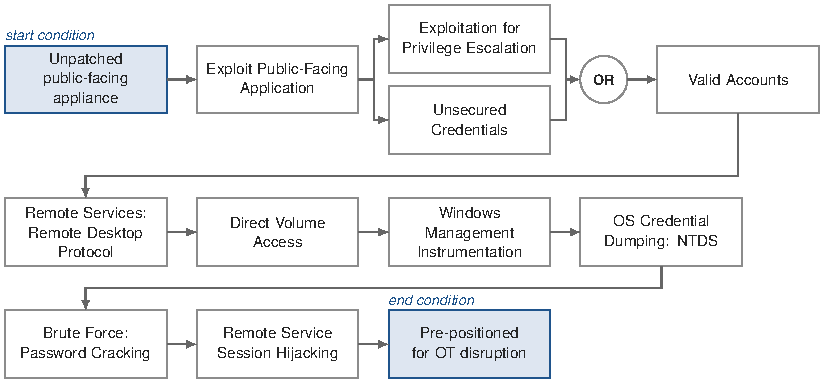
\includegraphics[width=\linewidth]{fig_3-1-3a_attack_flow_volt_typhoon}\\[1mm]
  {\scriptsize Volt Typhoon's intrusion as an \textbf{attack flow}}
\end{column}
\end{columns}
\takeaway{\textbf{Research question:} How does MTD perform against APT attackers?}
\end{frame}
\note[itemize]{
\item \textbf{0:15 to 1:30.} APT: a well-resourced attacker, often state-sponsored, pursuing one objective against one target over months or years (Alshamrani 2019). Espionage intrusions go undetected for a median of 122 days (Mandiant 2026).
\item Volt Typhoon held footholds in US critical infrastructure for at least five years, signing in with stolen valid accounts. Its reconnaissance stayed valid because the networks never changed.
\item MTD: change addresses, topology, software and credentials on a schedule, so what the attacker learned goes out of date even if it is never detected (Cho 2020).
\item Point at the attack flow: ``This is what a threat report gives us: the steps, in order, drawn by an analyst. It is the raw material of my attacker.''
\item The gap: MTD is proposed against APTs, but tested in simulation against attackers far simpler than an APT (Jalowski 2026). Read the research question aloud.
\item Transition: ``To test that, I need an MTD simulator and an attacker.''
}

% ============================================================================
\section{Previous work}
% Ch2: Figure 2.2, Table 2.1, Section 2.2.3.
\begin{frame}{MTDSim: seven MTD mechanisms, one scripted attacker}
\begin{columns}[T]
\begin{column}{0.44\textwidth}
\begin{itemize}
  \item \textbf{MTDSim} \src{Brown 2023; Zhang 2023; Tay 2024}
  \item \textbf{Host layer}: where hosts are
  \item \textbf{Service layer}: what runs on them
  \item \textbf{Baseline attacker}: six \textbf{attack actions}, fixed order
\end{itemize}
\end{column}
\begin{column}{0.53\textwidth}
  \centering
  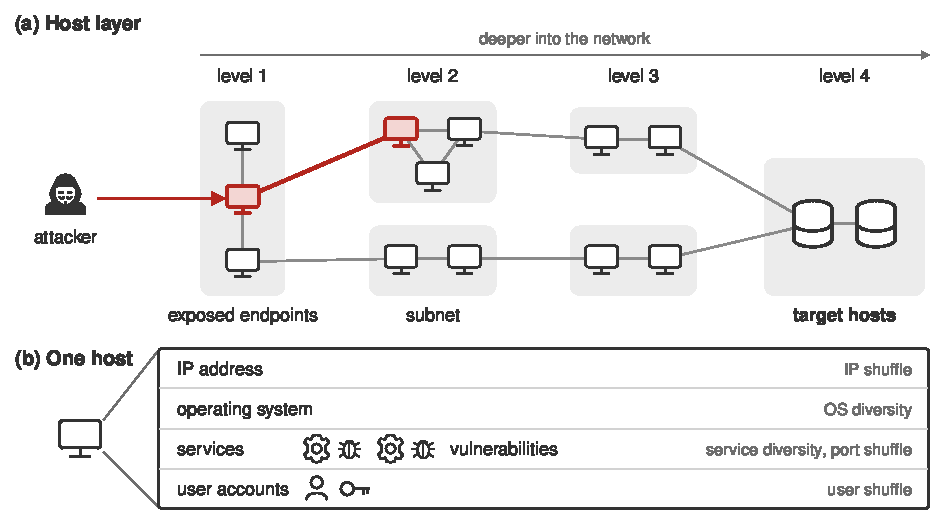
\includegraphics[width=\linewidth]{fig_2-2-1a_network_model}
\end{column}
\end{columns}
\end{frame}
\note[itemize]{
\item \textbf{1:30 to 2:30.} The work I inherit: Brown built MTDSim at UWA, Zhang added simulated time, Tay added MTDShield, a reinforcement-learning agent that picks which mechanism to deploy.
\item Panel (a): 50 hosts in four levels; the attacker enters at an exposed endpoint and works towards the target hosts.
\item Panel (b): each part of a host has a mechanism that moves it. Seven MTD mechanisms, one deployed every deployment interval (200\,s by default).
\item \textbf{The two layers the results hinge on}: host layer = IP shuffle and two topology shuffles; service layer = port shuffle, OS diversity, service diversity. Plus user shuffle on credentials.
\item Baseline attacker: scan host, enumerate host, scan port, exploit, brute force, scan neighbours; the same order every run.
\item Transition: ``Is a fixed procedure a fair stand-in for an APT?''
}

% ============================================================================
% Ch3: Tables 3.2 and 3.3.
\begin{frame}{Recent MTD attacker models lack most APT properties}
\centering
\small
\begin{tabular}{@{}l l c c c@{}}
\toprule
 & Property & Baseline attacker & Masud et al. & Kim et al. \\
 & & {\scriptsize 2023} & {\scriptsize 2025} & {\scriptsize 2026} \\
\midrule
1 & Campaign persistence & \yes & part & part \\
2 & Objective-specific behaviour & \no & \no & \no \\
3 & Choice of attack strategy & part & \no & \no \\
4 & Adaptivity to MTD disruption & part & \no & \no \\
5 & Detection avoidance & \no & \no & part \\
6 & Cost--benefit reasoning & \no & \no & \no \\
7 & Learning from past deployments & \no & \no & \no \\
8 & Deployment-strategy awareness & \no & \no & \no \\
\bottomrule
\end{tabular}\\[1mm]
{\scriptsize 1, 2, 4, 5: the APT definition \src{Alshamrani 2019; NIST 2011}. 3, 6, 7, 8: two MTD surveys \src{Cho 2020; Jalowski 2026}.}
\takeaway{\textbf{Gap}: how MTD performs against APT attackers is unmeasured.}
\end{frame}
\note[itemize]{
\item \textbf{2:30 to 3:30.} Eight properties: four from what an APT is, four that two MTD surveys say attacker models lack. Jalowski et al. call the attacker model ``the most glaring flaw in the MTD literature''.
\item I scored the baseline attacker and the two most recent MTD evaluations that describe their attacker in Kill Chain or ATT\&CK terms, the ones I expected to do best.
\item Read the result: at most one property in full, campaign persistence, only for the baseline attacker. None has objective-specific behaviour.
\item I targeted three: objective-specific behaviour, choice of attack strategy, adaptivity.
\item Likely question: ``How did you score them?'' $\to$ backup \textit{Scoring the eight properties}.
}

% ============================================================================
\section{Method}
% Ch4: Figure 4.1, Section 4.1, Table 4.1.
\begin{frame}{Build an APT attacker model from threat reports; run it in MTDSim}
\begin{columns}[T]
\begin{column}{0.60\textwidth}
  \centering
  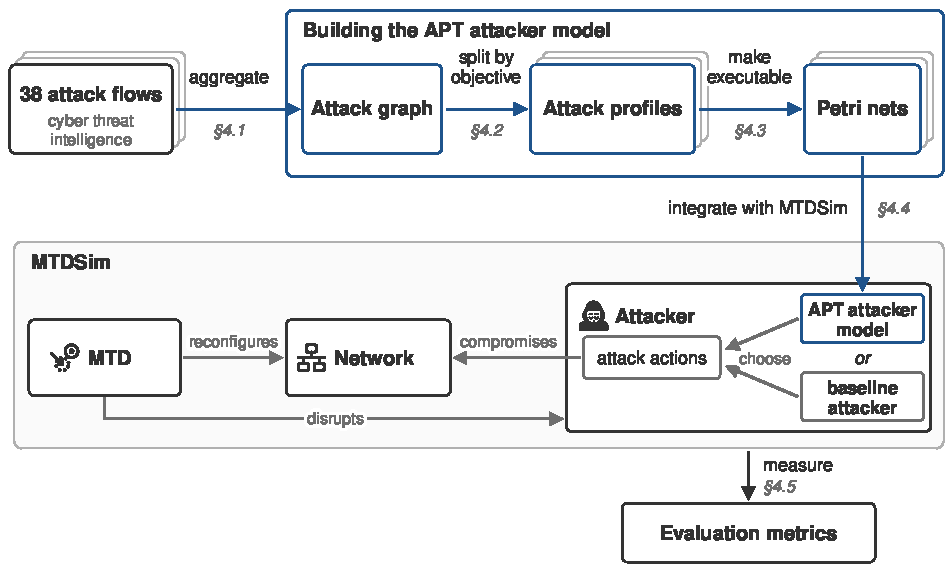
\includegraphics[width=\linewidth]{fig_4-0a_method_overview}
\end{column}
\begin{column}{0.37\textwidth}
\begin{itemize}
  \item \textbf{SQ1}: 38 attack flows $\to$ four \textbf{attack profiles} by objective
  \item \textbf{SQ2}: each runs as a Petri net
  \item \textbf{SQ3}: two attackers, same MTD
\end{itemize}
\vspace{2mm}
{\small
\begin{tabular}{@{}l l@{}}
c1 & stole data \\
c2 & impeded systems \\
c3 & both \\
c4 & neither \\
\end{tabular}}
\end{column}
\end{columns}
\end{frame}
\note[itemize]{
\item \textbf{3:30 to 4:45.} Three sub-questions, one pipeline: point left to right along the top row.
\item The 38 attack flows are analysts' hand-drawn graphs of reported intrusions, published by MITRE's Center for Threat-Informed Defense; the Volt Typhoon picture is one of the kind. Hand-drawn matters: automated extraction from report text is unreliable (best systems 80\,\% precision at 66\,\% recall on identifying techniques alone).
\item Aggregated into an attack graph over the 15 ATT\&CK tactics (what the attacker is trying to do: Initial Access, Lateral Movement, Exfiltration, \ldots). Tactics, not techniques: 88\,\% of technique-to-technique edges come from a single attack flow.
\item Split by two yes/no questions per attack flow: did it steal data, did it impede systems. c1 has 19 attack flows, c2 7, c3 7 (mostly ransomware), c4 5.
\item Transition: ``A graph does not run. Here is how it runs.''
}

% ============================================================================
% Ch4: Figure 4.5; Sections 4.3, 4.4.1 to 4.4.3; Figure 4.4(b).
\begin{frame}{A Petri net picks the next tactic; MTDSim carries it out}
\begin{columns}[T]
\begin{column}{0.62\textwidth}
  \centering
  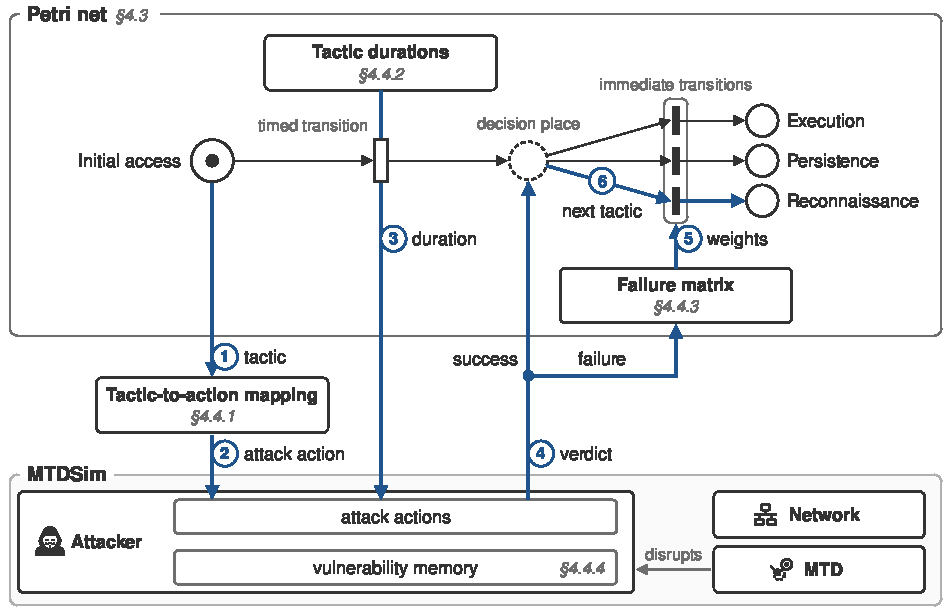
\includegraphics[width=\linewidth]{fig_4-4c_runtime_loop}
\end{column}
\begin{column}{0.35\textwidth}
\begin{itemize}
  \item Next tactic: drawn from the attack flows
  \item 7 of 15 tactics \textbf{unmapped}
  \item Timing and failures: declared
\end{itemize}
\end{column}
\end{columns}
\end{frame}
\note[itemize]{
\item \textbf{4:45 to 6:15.} Walk the loop once with your finger, steps 1 to 6: the token's tactic leaves the Petri net; the tactic-to-action mapping turns it into an attack action; it runs for the tactic duration; MTDSim returns success or failure; after a failure the failure matrix reweights; the token moves on.
\item Petri net: a generalised stochastic Petri net, the convention in MTD evaluation. Next tactic drawn in proportion to how many attack flows took that step, so runs differ.
\item Tactic-to-action mapping: 8 of 15 tactics run one of MTDSim's six attack actions. The other 7 (e.g.\ Exfiltration, Stealth) are unmapped and only take time. The ceiling: MTDSim's attack actions only find and compromise hosts, so the model steals no data. Say this plainly.
\item Threat reports record no timing and no failures. Tactic durations (up to 45\,s on average) and the failure matrix are declared before any result, then varied. Example: a failed Initial Access returns to Reconnaissance with weight 0.75, up from 0.06.
\item Likely questions: ``Why these durations?'' $\to$ backup \textit{Tactic durations}; ``Formal definition?'' $\to$ backup \textit{The Petri net}.
}

% ============================================================================
% Ch5: Table 5.1, Section 4.5.
\begin{frame}{Experiment: both attackers on the same 1\,000 networks}
\begin{columns}[T]
\begin{column}{0.52\textwidth}
\small
\begin{tabularx}{\linewidth}{@{}>{\bfseries}l >{\raggedright\arraybackslash}X@{}}
\toprule
Attacker & baseline; APT model, c1 to c4 \\
MTD & none; 7 mechanisms; 3 deployment strategies \\
Interval & 50 to 2\,000\,s \\
Seeds & 1\,000 per configuration \\
\bottomrule
\end{tabularx}
\end{column}
\begin{column}{0.45\textwidth}
\textbf{NCR}: share of hosts compromised\\[3mm]
\textbf{NCR reduction}\\[1mm]
$\displaystyle = 1 - \frac{\text{NCR under MTD}}{\text{NCR with no MTD}}$
\end{column}
\end{columns}
\end{frame}
\note[itemize]{
\item \textbf{6:15 to 7:00.} Keep this quick.
\item The design choice that matters: every configuration runs on the same 1\,000 seeds, so both attackers face the same 1\,000 networks. Differences come from the attacker, not the network. 1\,000 runs follows the recommendation for randomised algorithms (Arcuri and Briand).
\item MTD: none; each of the seven mechanisms alone; random and alternative rotation; MTDShield as released. Intervals 50, 100, 200, 500, 1\,000, 2\,000\,s.
\item Targeted scenario: a run ends at the first target host compromised, or at 15\,000\,s.
\item NCR, network compromise ratio (Zhang 2023). NCR reduction compares each attacker with its own runs with no MTD: 0 = no effect, 1 = nothing compromised.
\item MTD settings ranked by the Scott--Knott effect-size test; the two rankings compared with Spearman's $\rho$.
}

% ============================================================================
\section{Results}
% Ch5: Table 5.2, Figure 5.1(b), Section 5.2; Ch6 6.1.
\begin{frame}{No MTD: the APT attacker model acts more like an APT, but compromises less}
\small
\begin{tabularx}{\textwidth}{@{}>{\raggedright\arraybackslash}X >{\centering\arraybackslash}p{3.0cm} >{\centering\arraybackslash}p{2.4cm}@{}}
\toprule
 & APT attacker model & Baseline attacker \\
\midrule
Distinct openings (first 8 steps) & 179 to 947 & 3 \\
Attack actions per minute & 0.68 to 1.23 & 1.71 \\
Not flagged by a port-scan rule & 89 to 98\,\% & 82\,\% \\
\midrule
Runs reaching a target host (ASP) & 0.04 to 0.14 & 0.66 \\
Share of hosts compromised (NCR) & 0.15 to 0.21 & 0.50 \\
\bottomrule
\end{tabularx}
\normalsize
\takeaway{Same cause for both halves: its tactic durations and the order of its tactics.}
\end{frame}
\note[itemize]{
\item \textbf{7:00 to 8:15.} First, no MTD at all: does the model behave differently?
\item Row 1, choice of attack strategy: the baseline attacker's 1\,000 runs start the same way; the attack profiles' runs part ways by the second to fourth step. Ranges are over c1 to c4.
\item Rows 2 and 3, detection avoidance by proxy: it acts less often, and Snort's default port-scan rule (5 targets in 60\,s) would flag fewer of its attack actions. MTDSim has no IDS; say so.
\item Objective-specific behaviour (not on the slide): Exfiltration steps only in c1 and c3, Impact mostly in c2 and c3.
\item Bottom rows: it reaches a target in far fewer runs. Pre-empt the objection: ``Yes, with no MTD it is the weaker attacker. ASP and NCR alone would rate it weaker for exactly what makes it APT-like. With the baseline attacker's times it closes about two thirds of the gap.''
\item Transition: ``Two different attackers, the same networks. Now switch MTD on.''
\item Likely question: ``Isn't it just weaker?'' $\to$ backup \textit{Why it compromises less}.
}

% ============================================================================
% Ch5: Table 5.3 (200 s), Table F.4, Section 5.3.2.
\begin{frame}{Headline: the most effective MTD mechanism differs between the attackers}
\begin{columns}[T]
\begin{column}{0.56\textwidth}
\small
\begin{tabular}{@{}l >{\centering\arraybackslash}p{2.1cm} >{\centering\arraybackslash}p{2.1cm}@{}}
\toprule
NCR reduction at 200\,s & APT attacker model & Baseline attacker \\
\midrule
\multicolumn{3}{@{}l}{\textit{host layer}} \\
\quad IP shuffle & \textbf{96\,\% (1)} & 68\,\% (2) \\
\quad complete topology & \textbf{95\,\% (1)} & 42\,\% (3) \\
\quad host topology & \textbf{95\,\% (1)} & 38\,\% (3) \\
\multicolumn{3}{@{}l}{\textit{service layer}} \\
\quad service diversity & 36\,\% (4) & \textbf{92\,\% (1)} \\
\quad port shuffle & 20\,\% (6) & \textbf{91\,\% (1)} \\
\quad OS diversity & 7\,\% (7) & 68\,\% (2) \\
\multicolumn{3}{@{}l}{\textit{credentials}} \\
\quad user shuffle & $-10$\,\% (8) & $-5$\,\% (5) \\
\bottomrule
\end{tabular}\\[1mm]
{\scriptsize (rank) among all ten MTD settings}
\end{column}
\begin{column}{0.40\textwidth}
\begin{itemize}
  \item Rank 1 shares no mechanism
  \item Service diversity: 92 against 36\,\%
  \item Spearman's $\rho = 0.01$
\end{itemize}
\end{column}
\end{columns}
\end{frame}
\note[itemize]{
\item \textbf{8:15 to 9:45.} \textbf{This is the result. Slow down.}
\item Read the bold cells: against the APT attacker model, the host layer ranks first; against the baseline attacker, the service layer. Rank 1 shares no mechanism.
\item The one number: service diversity removes 92\,\% of the baseline attacker's NCR and 36\,\% of the APT attacker model's, on the same networks, with the same deployments.
\item $\rho = 0.01$: the two rankings are uncorrelated. Say ``do not agree'', not ``reversed''.
\item APT attacker model averaged over c1 to c4.
\item Only if asked: user shuffle is negative against the APT attacker model because it redraws accounts but leaves valid the ones the attacker holds, so each deployment is a fresh chance to log in.
\item Transition: ``Is that just the default interval?''
}

% ============================================================================
% Ch5: Figure 5.3 panels (a) and (b), redrawn per attacker from Table F.2; Figure 5.2 / Table F.1; Ch6 6.2.
\begin{frame}{The difference holds at every deployment interval}
\begin{columns}[T]
\begin{column}{0.58\textwidth}
\centering
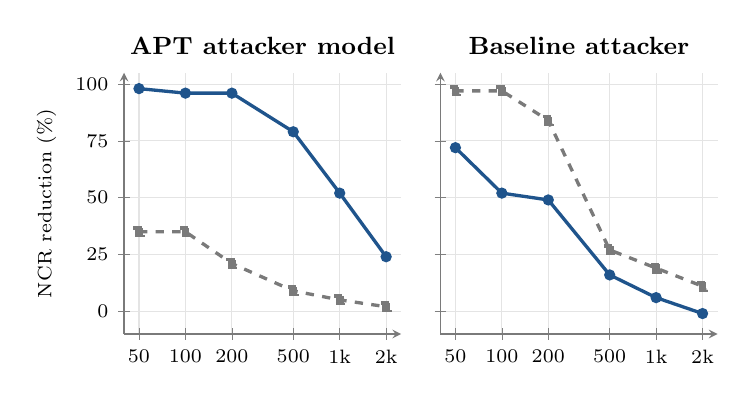
\begin{tikzpicture}
\begin{groupplot}[
  group style={group size=2 by 1, horizontal sep=5mm, y descriptions at=edge left},
  width=5.1cm, height=4.9cm, legend to name=layers,
  xmode=log, xmin=40, xmax=2500,
  xtick={50,100,200,500,1000,2000},
  xticklabels={50,100,200,500,1k,2k},
  ymin=-10, ymax=105, ytick={0,25,50,75,100},
  tick label style={font=\scriptsize},
  label style={font=\scriptsize},
  title style={font=\small\bfseries, yshift=-1mm},
  axis lines=left, axis line style={mid},
  grid=major, grid style={mid!20},
  legend style={font=\scriptsize, draw=none, legend columns=2, /tikz/every even column/.append style={column sep=4mm}},
]
\nextgroupplot[title={APT attacker model}, ylabel={NCR reduction (\%)}]
  \addplot[accent, very thick, mark=*, mark size=1.4pt] coordinates {(50,98)(100,96)(200,96)(500,79)(1000,52)(2000,24)};
  \addplot[mid, very thick, dashed, mark=square*, mark size=1.4pt] coordinates {(50,35)(100,35)(200,21)(500,9)(1000,5)(2000,2)};
\nextgroupplot[title={Baseline attacker}]
  \addplot[accent, very thick, mark=*, mark size=1.4pt] coordinates {(50,72)(100,52)(200,49)(500,16)(1000,6)(2000,-1)};
  \addplot[mid, very thick, dashed, mark=square*, mark size=1.4pt] coordinates {(50,97)(100,97)(200,84)(500,27)(1000,19)(2000,11)};
  \legend{host layer, service layer}
\end{groupplot}
\end{tikzpicture}\\[-0.5mm]
{\scriptsize Deployment interval (s, log scale)}\\[0.5mm]
\ref{layers}
\end{column}
\begin{column}{0.38\textwidth}
\textbf{Why} (measured at 2\,000\,s):
\begin{itemize}
  \item The service layer disrupts only port scans, exploits and brute force
  \item Blocks an attack action: 95\,\% baseline, 15\,\% APT model
  \item Host layer costs the APT model 242 to 324\,s
\end{itemize}
\end{column}
\end{columns}
\end{frame}
\note[itemize]{
\item \textbf{9:45 to 11:15.} Left: in each panel, which line is on top? APT attacker model: host layer, at every interval. Baseline attacker: service layer, at every interval. Each line is the mean over the layer's mechanisms.
\item The host layer keeps at least half of the APT attacker model's NCR off up to 1\,000\,s; the service layer does that for the baseline attacker only up to 200\,s.
\item Why: a deployment disrupts an attacker only if it lands while the attacker is doing what that layer breaks. The baseline attacker scans ports, exploits and brute-forces back to back; the APT attacker model sits mostly in unmapped tactics, which run no attack action.
\item A host-layer deployment costs the APT attacker model 242 to 324\,s: it has no host until its Petri net next reaches Lateral Movement. The baseline attacker loses none, because its procedure re-enumerates a host at once.
\item Say ``likely'': the tactic durations and the order of the tactics most likely explain it; no run separates the two.
\item Likely question: ``Does the host layer just stop it getting in?'' $\to$ backup \textit{Footholds under the host layer}. Answer: largely yes, at short intervals.
}

% ============================================================================
\section{So what}
% Ch6 6.4; Table F.2 (200 s); Appendix E.5.
\begin{frame}{The attacker model can decide which MTD looks best}
\begin{columns}[T]
\begin{column}{0.46\textwidth}
\centering
\small
\textbf{MTDShield}, learned against the baseline attacker\\[2mm]
\begin{tabular}{@{}l r r@{}}
\toprule
NCR reduction, 200\,s & Baseline & APT model \\
\midrule
MTDShield & \textbf{68\,\%} & 28\,\% \\
random deployment & 33\,\% & \textbf{75\,\%} \\
\bottomrule
\end{tabular}
\end{column}
\begin{column}{0.50\textwidth}
\begin{itemize}
  \item Test a learned strategy on an attacker it was not trained on
  \item Report a ranking with its attacker model
  \item Cost depends on the attacker model
\end{itemize}
\end{column}
\end{columns}
\takeaway{One simplified attacker cannot tell you how MTD performs against an APT.}
\end{frame}
\note[itemize]{
\item \textbf{11:15 to 12:45.} The ``so what'' for anyone who evaluates MTD.
\item MTDShield was trained and tested by Tay against the baseline attacker. It deploys service diversity in 70\,\% or more of its decisions against either attacker. Against the APT attacker model, random deployment does almost three times better. Most likely it learned the mechanism that disrupts its training attacker: a test in the training environment is a test on training data.
\item Fair to Tay: it runs as released, outside its training conditions; this bounds MTDShield as released, not retrained.
\item Recommendation 1: test a learned deployment strategy against an attacker model it was not trained on, beside random deployment over the same mechanisms.
\item Recommendation 2: report each ranking with the attacker model behind it; compare across studies only on a shared attacker model.
\item Recommendation 3, cost: to halve NCR, service diversity deploys every 1\,000\,s against the baseline attacker, but every 100\,s against the APT attacker model: ten times the overhead.
\item Optional question to the room: ``If you were choosing an MTD for a real network, which attacker model would you trust?''
}

% ============================================================================
\section{Conclusion}
% Ch6 6.5 (limitations; T1, T4, T5, T10, T11).
\begin{frame}{Limitations}
\begin{itemize}
  \item One simulator, one network size, no deployment cost
  \item Six attack actions: no data theft, no IDS
  \item Declared durations and failure matrix
  \item 38 attack flows
  \item Cause not isolated
\end{itemize}
\end{frame}
\note[itemize]{
\item \textbf{12:45 to 13:45.} State these yourself before anyone asks; examiners mark you for it.
\item One simulator: every claim holds in MTDSim, on its default 50-host network, with deployments that cost nothing.
\item MTDSim's six attack actions cap the model: 7 of 15 tactics unmapped, so no data theft, no impact, and no IDS to evade.
\item Declared values: tactic durations and failure matrix are judgement where threat reports are silent, fixed before any result. Only the 45\,s duration moves NCR much, and the ranking holds from a quarter to four times it.
\item Small corpus: 38 attack flows, 18 attributed to a known group; three attack profiles rest on 5 to 7.
\item Cause not isolated: tactic durations or the order of tactics. MTDSim's disruption rules were written for the baseline attacker; an APT holding a host through Command and Control might survive an IP shuffle. Both attackers meet the same rules, so the comparison is fair.
\item The headline does not say ``MTD fails against APTs'' or ``my attacker is the realistic one''. It says the ranking \emph{can depend} on the attacker model.
\item Likely question: ``How do you know the code does what you say?'' $\to$ backup \textit{Verification}.
}

% ============================================================================
% Ch7 drafting notes; Table 6.1; Section 7.2.
\begin{frame}{In MTDSim, the most effective MTD depends on the attacker model}
\begin{itemize}
  \item \textbf{Built}: an APT attacker model from 38 attack flows, runnable in MTDSim
  \item \textbf{Found}: host layer against it, service layer against the baseline attacker
  \item \textbf{Next}: richer attack actions, an IDS, deployment cost
\end{itemize}
\takeaway{Evaluate MTD against attacker models grounded in documented behaviour.}
\end{frame}
\note[itemize]{
\item \textbf{13:45 to 14:45.} Answer the research question in one sentence, then the two contributions. No new numbers; the audience has 92 against 36\,\%.
\item Contribution 1: the APT attacker model, which any MTDSim study can run in place of the baseline attacker. Two of the eight properties in full and three in part, against at most one in full for three recent models. A proof of concept, built, run and open-sourced; not a claim that it reproduces APT behaviour.
\item Contribution 2: the finding. At every deployment interval, the host layer disrupts the APT attacker model most and the service layer the baseline attacker.
\item Future work: attack actions for actions on objectives, and an IDS; separate the tactic durations from the order of tactics; deployment cost; other networks; MTDShield retrained against the APT attacker model.
\item Then move to the questions slide.
}

% ============================================================================
\begin{frame}[plain,noframenumbering]
\centering
\vfill
{\Huge\color{accent}\textbf{Questions?}}\\[8mm]
{\large How does MTD perform against APT attackers?}\\[2mm]
{\normalsize In MTDSim, it depends on which attacker it is tested against.}\\[10mm]
{\small\color{mid} Marc Labouchardiere \quad\textbullet\quad Supervisor: Dr Jin B. Hong}\\[1mm]
{\small\color{mid} Code and experiments: github.com/marc-la/MTDSim}
\vfill
\end{frame}
\note[itemize]{
\item Leave this up during questions.
\item Q\&A map: weaker attacker $\to$ \textit{Why it compromises less}; footholds $\to$ \textit{Footholds}; durations $\to$ \textit{Tactic durations}; components $\to$ \textit{Ablations}; per profile $\to$ \textit{Each attack profile}; scoring $\to$ \textit{Scoring}; Petri net $\to$ \textit{The Petri net}; MTDShield $\to$ \textit{MTDShield as run}; ASP $\to$ \textit{Disruption and ASP}; earlier numbers $\to$ \textit{Verification}.
}

% ============================================================================
% =========================== BACKUP SLIDES ==================================
% ============================================================================
\appendix
\setbeamertemplate{footline}{\hfill{\scriptsize\color{mid}Backup \insertframenumber}\hspace*{4mm}\vspace{2mm}}

% Ch6 6.1; Appendix G.3, Tables G.5 and G.6; T2.
\begin{frame}{Backup: why the APT attacker model compromises less with no MTD}
\begin{itemize}
  \item Unmapped tactics take 34 to 57\,\% of an attack profile's run, and 15 to 30\,\% of its attack actions fail because their preconditions are missing (e.g.\ exploit before scan port)
  \item Rerun with the baseline attacker's times in place of its tactic durations, same order of tactics: ASP rises from 0.09 to 0.45, against the baseline attacker's 0.66, closing 63\,\% of the gap
  \item The order of its tactics most likely accounts for the rest
  \item The rankings compare each attacker with its own NCR with no MTD, so the lower starting point is unlikely to decide which mechanism ranks first
\end{itemize}
\vfill{\scriptsize Dissertation Section 6.1, Appendix G.3, threat T2. Appendix G analyses were chosen after the results were seen (T9).}
\end{frame}

% Appendix G.4, Table G.7.
\begin{frame}{Backup: footholds under the host layer}
\begin{itemize}
  \item Under the three host-layer mechanisms at 50 to 200\,s, 70 to 89\,\% of the APT attacker model's runs compromise no host, against 3 to 20\,\% of the baseline attacker's
  \item With no MTD: 1\,\% and none
  \item So the host layer disrupts the APT attacker model mostly \emph{before} its first foothold: after a host-layer deployment it has no host until its Petri net next reaches Lateral Movement
  \item From 500\,s the share falls for both attackers, and the host layer still ranks first against the APT attacker model
\end{itemize}
\vfill{\scriptsize Dissertation Appendix G.4 (post hoc, T9); the claim stands on Chapter 5 without it.}
\end{frame}

% Appendix D.1, Tables D.3 and D.4.
\begin{frame}{Backup: are the declared tactic durations driving the result?}
\begin{columns}[T]
\begin{column}{0.48\textwidth}
\small
\begin{tabular}{@{}l r r r@{}}
\toprule
Mean duration (band) & low & declared & high \\
\midrule
4.5\,s (2.25 to 9) & 0.165 & 0.163 & 0.159 \\
35\,s (17.5 to 70) & 0.172 & 0.163 & 0.145 \\
36\,s (18 to 72) & 0.170 & 0.163 & 0.148 \\
45\,s (11.25 to 180) & \textbf{0.267} & 0.163 & \textbf{0.059} \\
\bottomrule
\end{tabular}\\[1mm]
{\scriptsize NCR with no MTD, each value moved alone, 400 runs per cell.}
\end{column}
\begin{column}{0.48\textwidth}
\begin{itemize}
  \item Bands fixed before the run; one value moved at a time
  \item Only the 45\,s (Persistence, Stealth, Command and Control) moves NCR much: Command and Control is the only tactic that finds new hosts
  \item At a quarter and four times the 45\,s, rank 1 still shares no mechanism with the baseline attacker's, and the host layer still ranks above the service layer ($\rho = 0.03$ and $-0.03$)
  \item Untested: interactions between values
\end{itemize}
\end{column}
\end{columns}
\vfill{\scriptsize Dissertation Appendix D.1, threat T4.}
\end{frame}

% Section 5.4, Table 5.4.
\begin{frame}{Backup: what each component of the APT attacker model changes}
\centering
\small
\begin{tabular}{@{}l l r r r@{}}
\toprule
Component removed & MTD & NCR with & without & Cohen's $d$ \\
\midrule
Attack profiles (use the whole attack graph) & no MTD & 0.171 & 0.189 & \textbf{$-0.28$} \\
 & IP shuffle, 200\,s & 0.007 & 0.013 & \textbf{$-0.47$} \\
 & OS diversity, 200\,s & 0.159 & 0.174 & \textbf{$-0.26$} \\
\midrule
Failure matrix & no MTD & 0.171 & 0.167 & $+0.07$ \\
 & IP shuffle, 200\,s & 0.007 & 0.006 & $+0.13$ \\
\midrule
Vulnerability memory & no MTD & 0.171 & 0.169 & $+0.04$ \\
 & service diversity, 200\,s & 0.109 & 0.106 & $+0.07$ \\
\bottomrule
\end{tabular}\\[2mm]
\raggedright
\begin{itemize}
  \item Bold: not negligible ($|d| > 0.2$). The failure matrix changes \emph{where} the attacker goes after a failure (back to Reconnaissance 76 to 83\,\% vs 8 to 10\,\%), not what it achieves
  \item Without the attack profiles, the same three host-layer mechanisms still rank first
\end{itemize}
\end{frame}

% Figure 5.4.
\begin{frame}{Backup: each attack profile against the baseline attacker}
\centering
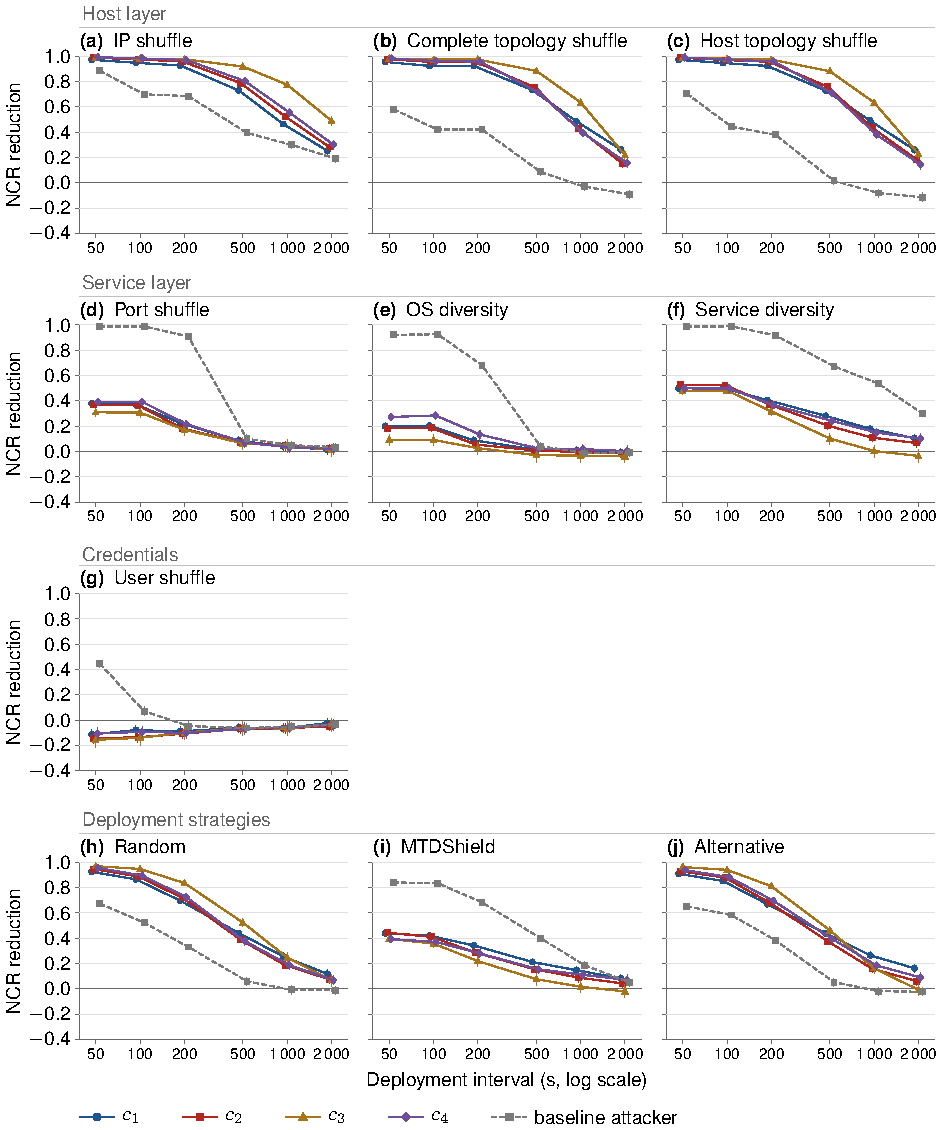
\includegraphics[height=0.80\textheight]{fig_5-3-3b_interval_mechanisms}\\
{\scriptsize At 50 to 200\,s the four attack profiles differ from one another less than the baseline attacker differs from the nearest of them (dissertation Figure 5.4).}
\end{frame}

% Table 6.1, Section 3.3.2, T7.
\begin{frame}{Backup: scoring the eight properties}
\centering
\small
\begin{tabular}{@{}l c c c c c c c c@{}}
\toprule
 & 1 & 2 & 3 & 4 & 5 & 6 & 7 & 8 \\
Attacker model & Pers. & Obj. & Strat. & Adapt. & Detect. & Cost & Learn. & Deploy. \\
\midrule
Baseline attacker (2023) & \yes & \no & part & part & \no & \no & \no & \no \\
Masud et al.\ (2025) & part & \no & \no & \no & \no & \no & \no & \no \\
Kim et al.\ (2026) & part & \no & \no & \no & part & \no & \no & \no \\
\textbf{APT attacker model} & \yes & part & \yes & part & part & \no & \no & \no \\
\bottomrule
\end{tabular}\\[2mm]
\raggedright
\begin{itemize}
  \item Each property split into predicates; \yes{} = every predicate true of the model's own behaviour; part = a behaviour predicate true, but set by a fixed rule or assumed
  \item One scorer, checked by blind scoring with language models (dissertation Appendix B)
  \item Adaptivity is in part because the failure matrix is a fixed rule of mine; detection avoidance in part because MTDSim has no IDS
\end{itemize}
\end{frame}

% Section 4.3, Equations 4.2 and 4.4, Figure 4.4.
\begin{frame}{Backup: the Petri net}
\begin{columns}[T]
\begin{column}{0.52\textwidth}
\centering
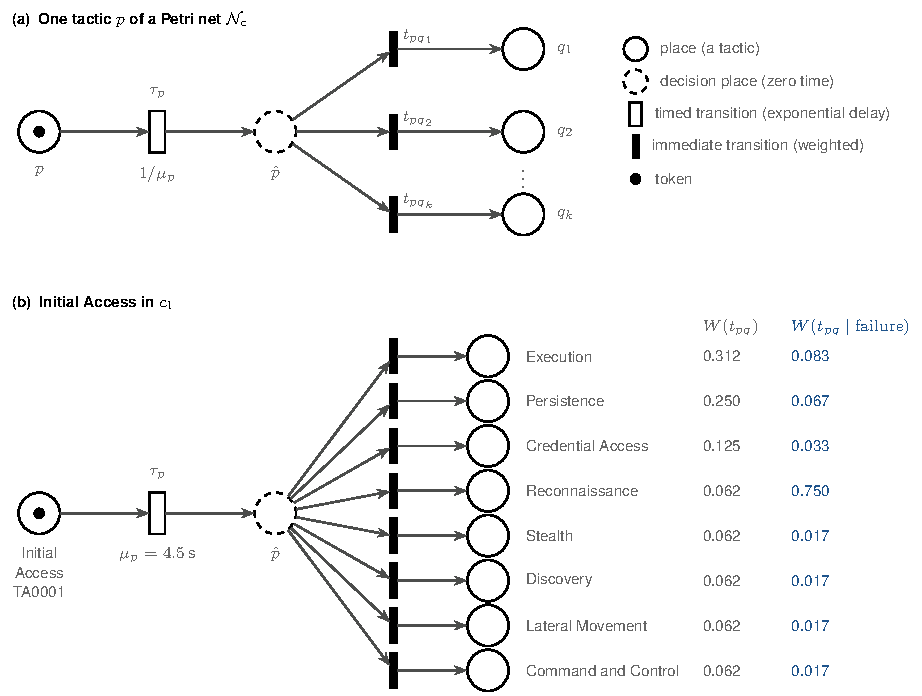
\includegraphics[width=\linewidth]{fig_4-3a_gspn_gadget}
\end{column}
\begin{column}{0.45\textwidth}
\small
Generalised stochastic Petri net \src{Ajmone Marsan 1995}, extended with the failure matrix $F$:
\[(P, T, I, O, W, M_0, F)\]
Base weight of the move from tactic $p$ to $q$:
\[W(t_{pq}) = \frac{n(p,q)}{\sum_{q'} n(p,q')}\]
with $n(p,q)$ the attack flows that draw $p \to q$. After a failed attack action:
\[W(t_{pq}\mid\text{failure}) = \frac{W(t_{pq})\,F(p,q)}{\sum_{q'} W(t_{pq'})\,F(p,q')}\]
One token, starting on Reconnaissance.
\end{column}
\end{columns}
\end{frame}

% Table 4.2, Figure 4.6.
\begin{frame}{Backup: tactic durations and the tactic-to-action mapping}
\begin{columns}[T]
\begin{column}{0.50\textwidth}
\small
\begin{tabular}{@{}>{\raggedright\arraybackslash}p{0.72\linewidth} r@{}}
\toprule
Tactics & Mean (s) \\
\midrule
Initial Access, Privilege Escalation, Credential Access, Lateral Movement {\scriptsize(MTDSim's exploit)} & 4.5 \\
Reconnaissance, Discovery {\scriptsize(MTDSim's three scans)} & 35 \\
Persistence, Stealth, Command and Control & 45 \\
Collection, Exfiltration, Impact & 36 \\
Execution, Defense Impairment & 22.5 \\
Resource Development & 0 \\
\bottomrule
\end{tabular}\\[1mm]
{\scriptsize Last four rows: judgement, kept on the baseline attacker's time scale and under the 200\,s default interval.}
\end{column}
\begin{column}{0.46\textwidth}
\centering
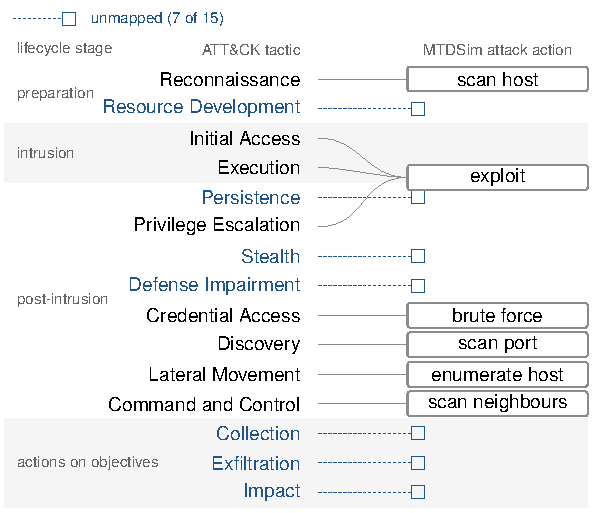
\includegraphics[width=\linewidth]{fig_4-4a_controller_mapping}
\end{column}
\end{columns}
\end{frame}

% Appendix E.4 and E.5.
\begin{frame}{Backup: MTDShield as run}
\begin{itemize}
  \item Run as released by Tay (2024); correcting the release would make it my agent, not Tay's
  \item Trained at one deployment interval, against the baseline attacker, on 100-host networks
  \item Known limits of the release: published scores produced with exploration at one; four evaluation inputs read as zero; ``do nothing'' never a learning target
  \item Its detection input reads an unmapped tactic as ``nothing detected''
  \item So the result bounds MTDShield \emph{as released}, not MTDShield retrained against the APT attacker model
\end{itemize}
\vfill{\scriptsize Dissertation Appendix E, threat T12.}
\end{frame}

% Figure 5.2; Appendix F.1, Table F.3.
\begin{frame}{Backup: disruption per MTD deployment, and ASP}
\begin{columns}[T]
\begin{column}{0.58\textwidth}
\centering
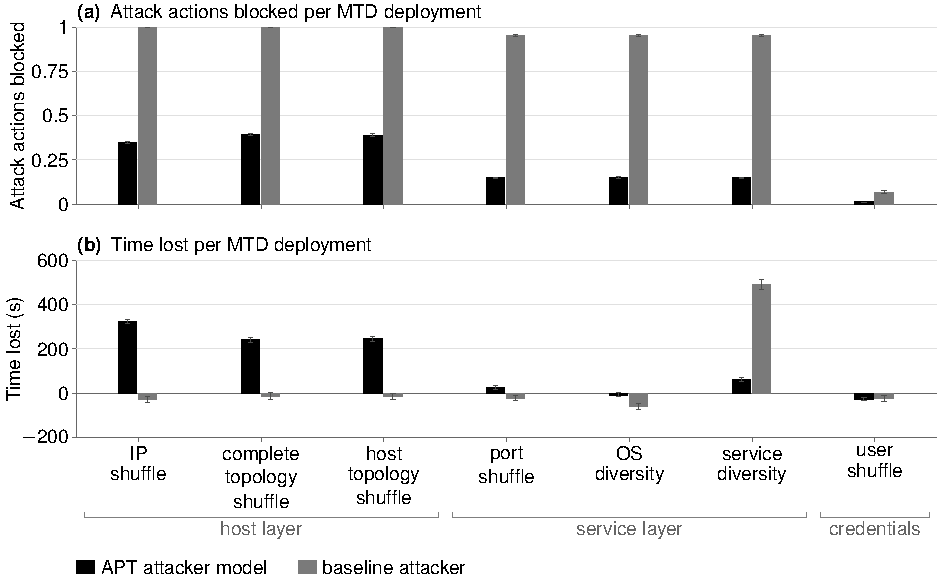
\includegraphics[width=\linewidth]{fig_5-2-2a_disruption_response}
\end{column}
\begin{column}{0.39\textwidth}
\begin{itemize}
  \item Measured at 2\,000\,s, because the next deployment caps time lost at the interval
  \item The baseline attacker's time lost is at or below zero after the first deployment: sent back to scan host, it gets a second attempt at its first host, as MTDSim intends
  \item On ASP reduction the layer order also holds against each attacker (Table F.3)
\end{itemize}
\end{column}
\end{columns}
\end{frame}

% T3.
\begin{frame}{Backup: verification, and why no comparison with earlier MTDSim numbers}
\begin{itemize}
  \item An event tracer replays any run step by step, across Petri net, attacker and MTD
  \item MTDSim's code audited against what its papers describe; unit tests of the Petri net and the simulator
  \item Fixed seeds reproduce every run exactly
  \item Defects found in MTDSim were repaired before the evaluation, so results are not compared numerically with Zhang (2023) or Tay (2024)
\end{itemize}
\vfill{\scriptsize Dissertation threat T3.}
\end{frame}

\begin{frame}{References}
\scriptsize
\begin{itemize}
  \item[] A.~Alshamrani et al., ``A survey on advanced persistent threats,'' \emph{IEEE Commun.\ Surveys Tuts.}, 21(2), 2019.
  \item[] M.~Ajmone Marsan et al., \emph{Modelling with Generalized Stochastic Petri Nets}, Wiley, 1995.
  \item[] A.~Brown, T.-W.~Lee and J.~B.~Hong, ``Evaluating moving target defenses against realistic attack scenarios,'' EnCyCriS, 2023.
  \item[] Center for Threat-Informed Defense, ``Attack Flow,'' MITRE, v3.2.0, 2025.
  \item[] J.-H.~Cho et al., ``Toward proactive, adaptive defense: A survey on moving target defense,'' \emph{IEEE Commun.\ Surveys Tuts.}, 22(1), 2020.
  \item[] CISA et al., ``PRC state-sponsored actors compromise and maintain persistent access to U.S.\ critical infrastructure,'' Advisory AA24-038A, 2024.
  \item[] {\L}.~Jalowski et al., ``Rethinking the security assurances of MTD: A gap analysis for network defense,'' \emph{Future Internet}, 18(2), 2026.
  \item[] M.~Kim et al., ``MTD in depth: Multi-phased moving target defense techniques against cyber-attacks based on cyber kill chain,'' \emph{FGCS}, 181, 2026.
  \item[] M.~T.~Masud et al., ``Vulnerability defence using hybrid moving target defence in Internet of Things systems,'' \emph{Computers \& Security}, 153, 2025.
  \item[] Joint Task Force, ``Managing information security risk,'' NIST SP 800-39, 2011.
  \item[] C.~Tantithamthavorn et al., ``An empirical comparison of model validation techniques for defect prediction models,'' \emph{IEEE TSE}, 43(1), 2017.
  \item[] J.~K.~Tay, ``Using artificial intelligence to automate the deployment of moving target defence operations,'' UWA research report, 2024.
  \item[] W.~Zhang, ``Evaluating multiple moving target defence in the time domain,'' Master's thesis, UWA, 2023.
\end{itemize}
\end{frame}

\end{document}
"  (twice)
% Slides carry prompts only; what to say is in each frame's \note.
% Every number on a slide is taken from the dissertation; the table or
% figure it comes from is named in the frame's comment.
\documentclass[aspectratio=169,11pt]{beamer}

\usepackage[T1]{fontenc}
\usepackage[scaled=0.92]{helvet}   % the figures' face
\usepackage{booktabs}
\usepackage{array}
\usepackage{tabularx}
\usepackage{pifont}
\usepackage{pgfplots}
\pgfplotsset{compat=1.17}
\usepgfplotslibrary{groupplots}
\usepackage{appendixnumberbeamer}   % "n / 12" counts the main slides only
\graphicspath{{../figures/}}

\ifdefined\withnotes
  \setbeameroption{show notes}
\fi

% --- look: plain, legible, one accent ---------------------------------------
\definecolor{accent}{RGB}{31,84,140}
\definecolor{mid}{RGB}{122,122,122}
\setbeamertemplate{navigation symbols}{}
\setbeamercolor{frametitle}{fg=accent}
\setbeamerfont{frametitle}{size=\large,series=\bfseries}
\setbeamercolor{structure}{fg=accent}
\setbeamertemplate{itemize items}{\color{accent}\textbullet}
\setbeamertemplate{itemize subitem}{\color{mid}--}
\setbeamersize{text margin left=8mm,text margin right=8mm}

% --- footer: the talk's timeline (sections, one dot per slide) + n / 12 -----
\useoutertheme[subsection=false]{miniframes}
\setbeamertemplate{headline}{}
\setbeamertemplate{mini frames}[default]
\setbeamercolor{section in head/foot}{fg=accent}
\setbeamercolor{mini frame}{fg=accent}
\setbeamerfont{section in head/foot}{size=\scriptsize}
\setbeamertemplate{footline}{%
  \begin{beamercolorbox}[wd=\paperwidth,ht=4mm,dp=3.6mm]{section in head/foot}%
    \hspace*{2mm}\insertnavigation{0.82\paperwidth}\hfill
    {\scriptsize\color{mid}\insertframenumber\,/\,\inserttotalframenumber}\hspace*{4mm}%
  \end{beamercolorbox}}

\newcommand{\src}[1]{{\scriptsize\color{mid}[#1]}}
\newcommand{\yes}{\ding{51}}
\newcommand{\no}{{\color{mid}\ding{55}}}
\newcommand{\takeaway}[1]{\vfill{\color{accent}\rule{\linewidth}{0.4pt}}\\[1mm]#1\vspace{1mm}}

\title{Evaluating moving target defence against advanced persistent threat attackers modelled on documented intrusion campaigns}
\author{Marc Labouchardiere\\[1mm]{\small Supervisor: Dr Jin B. Hong}}
\institute{\small Honours seminar, The University of Western Australia}
\date{\small 2026}

\begin{document}

% ============================================================================
\begin{frame}[plain,noframenumbering]
  \titlepage
\end{frame}
\note[itemize]{
\item \textbf{0:00 to 0:15.} Name, supervisor.
\item One line: ``I test whether MTD's measured effectiveness survives a change of attacker.''
\item The footer is the talk's timeline: six parts, one dot per slide.
}

% ============================================================================
\section{Motivation}
% Ch1; ch3 3.1.1 and 3.1.3; Figure 3.2.
\begin{frame}{MTD is proposed against APT attackers, but rarely tested against one}
\begin{columns}[T]
\begin{column}{0.44\textwidth}
\begin{itemize}
  \item \textbf{Advanced persistent threat (APT)}: one target, months to years
  \item Volt Typhoon: five years inside US infrastructure \src{CISA 2024}
  \item \textbf{Moving target defence (MTD)}: keep the network moving
  \item Tested against simple, scripted attackers
\end{itemize}
\end{column}
\begin{column}{0.53\textwidth}
  \centering
  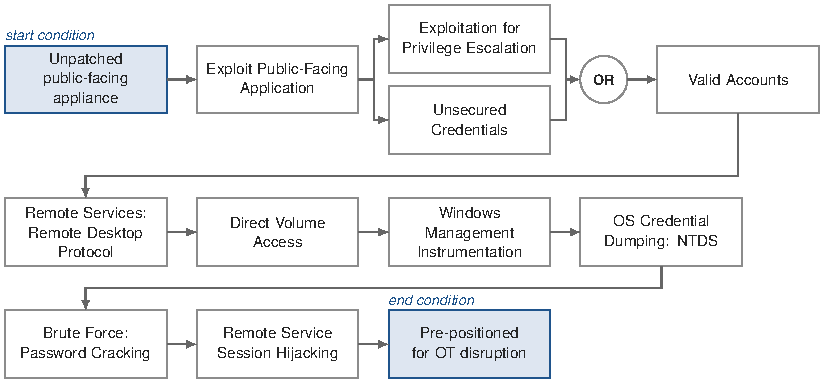
\includegraphics[width=\linewidth]{fig_3-1-3a_attack_flow_volt_typhoon}\\[1mm]
  {\scriptsize Volt Typhoon's intrusion as an \textbf{attack flow}}
\end{column}
\end{columns}
\takeaway{\textbf{Research question:} How does MTD perform against APT attackers?}
\end{frame}
\note[itemize]{
\item \textbf{0:15 to 1:30.} APT: a well-resourced attacker, often state-sponsored, pursuing one objective against one target over months or years (Alshamrani 2019). Espionage intrusions go undetected for a median of 122 days (Mandiant 2026).
\item Volt Typhoon held footholds in US critical infrastructure for at least five years, signing in with stolen valid accounts. Its reconnaissance stayed valid because the networks never changed.
\item MTD: change addresses, topology, software and credentials on a schedule, so what the attacker learned goes out of date even if it is never detected (Cho 2020).
\item Point at the attack flow: ``This is what a threat report gives us: the steps, in order, drawn by an analyst. It is the raw material of my attacker.''
\item The gap: MTD is proposed against APTs, but tested in simulation against attackers far simpler than an APT (Jalowski 2026). Read the research question aloud.
\item Transition: ``To test that, I need an MTD simulator and an attacker.''
}

% ============================================================================
\section{Previous work}
% Ch2: Figure 2.2, Table 2.1, Section 2.2.3.
\begin{frame}{MTDSim: seven MTD mechanisms, one scripted attacker}
\begin{columns}[T]
\begin{column}{0.44\textwidth}
\begin{itemize}
  \item \textbf{MTDSim} \src{Brown 2023; Zhang 2023; Tay 2024}
  \item \textbf{Host layer}: where hosts are
  \item \textbf{Service layer}: what runs on them
  \item \textbf{Baseline attacker}: six \textbf{attack actions}, fixed order
\end{itemize}
\end{column}
\begin{column}{0.53\textwidth}
  \centering
  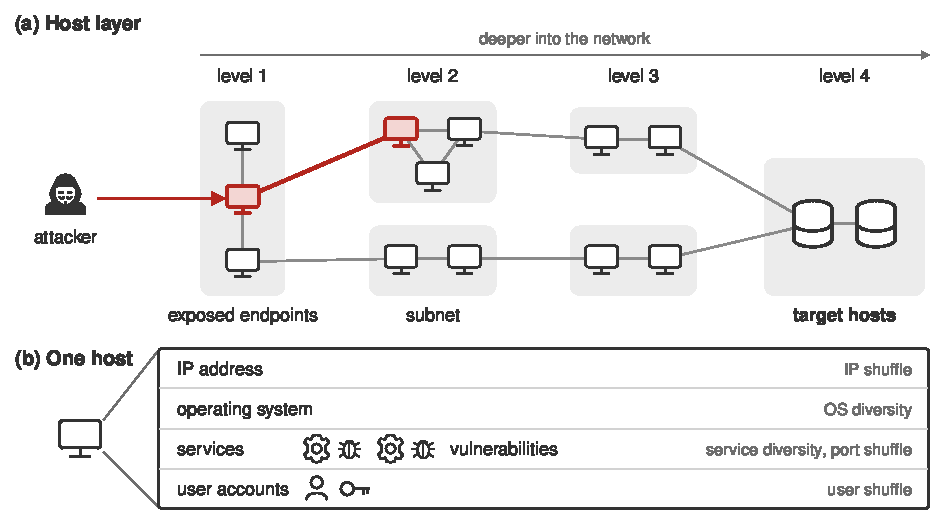
\includegraphics[width=\linewidth]{fig_2-2-1a_network_model}
\end{column}
\end{columns}
\end{frame}
\note[itemize]{
\item \textbf{1:30 to 2:30.} The work I inherit: Brown built MTDSim at UWA, Zhang added simulated time, Tay added MTDShield, a reinforcement-learning agent that picks which mechanism to deploy.
\item Panel (a): 50 hosts in four levels; the attacker enters at an exposed endpoint and works towards the target hosts.
\item Panel (b): each part of a host has a mechanism that moves it. Seven MTD mechanisms, one deployed every deployment interval (200\,s by default).
\item \textbf{The two layers the results hinge on}: host layer = IP shuffle and two topology shuffles; service layer = port shuffle, OS diversity, service diversity. Plus user shuffle on credentials.
\item Baseline attacker: scan host, enumerate host, scan port, exploit, brute force, scan neighbours; the same order every run.
\item Transition: ``Is a fixed procedure a fair stand-in for an APT?''
}

% ============================================================================
% Ch3: Tables 3.2 and 3.3.
\begin{frame}{Recent MTD attacker models lack most APT properties}
\centering
\small
\begin{tabular}{@{}l l c c c@{}}
\toprule
 & Property & Baseline attacker & Masud et al. & Kim et al. \\
 & & {\scriptsize 2023} & {\scriptsize 2025} & {\scriptsize 2026} \\
\midrule
1 & Campaign persistence & \yes & part & part \\
2 & Objective-specific behaviour & \no & \no & \no \\
3 & Choice of attack strategy & part & \no & \no \\
4 & Adaptivity to MTD disruption & part & \no & \no \\
5 & Detection avoidance & \no & \no & part \\
6 & Cost--benefit reasoning & \no & \no & \no \\
7 & Learning from past deployments & \no & \no & \no \\
8 & Deployment-strategy awareness & \no & \no & \no \\
\bottomrule
\end{tabular}\\[1mm]
{\scriptsize 1, 2, 4, 5: the APT definition \src{Alshamrani 2019; NIST 2011}. 3, 6, 7, 8: two MTD surveys \src{Cho 2020; Jalowski 2026}.}
\takeaway{\textbf{Gap}: how MTD performs against APT attackers is unmeasured.}
\end{frame}
\note[itemize]{
\item \textbf{2:30 to 3:30.} Eight properties: four from what an APT is, four that two MTD surveys say attacker models lack. Jalowski et al. call the attacker model ``the most glaring flaw in the MTD literature''.
\item I scored the baseline attacker and the two most recent MTD evaluations that describe their attacker in Kill Chain or ATT\&CK terms, the ones I expected to do best.
\item Read the result: at most one property in full, campaign persistence, only for the baseline attacker. None has objective-specific behaviour.
\item I targeted three: objective-specific behaviour, choice of attack strategy, adaptivity.
\item Likely question: ``How did you score them?'' $\to$ backup \textit{Scoring the eight properties}.
}

% ============================================================================
\section{Method}
% Ch4: Figure 4.1, Section 4.1, Table 4.1.
\begin{frame}{Build an APT attacker model from threat reports; run it in MTDSim}
\begin{columns}[T]
\begin{column}{0.60\textwidth}
  \centering
  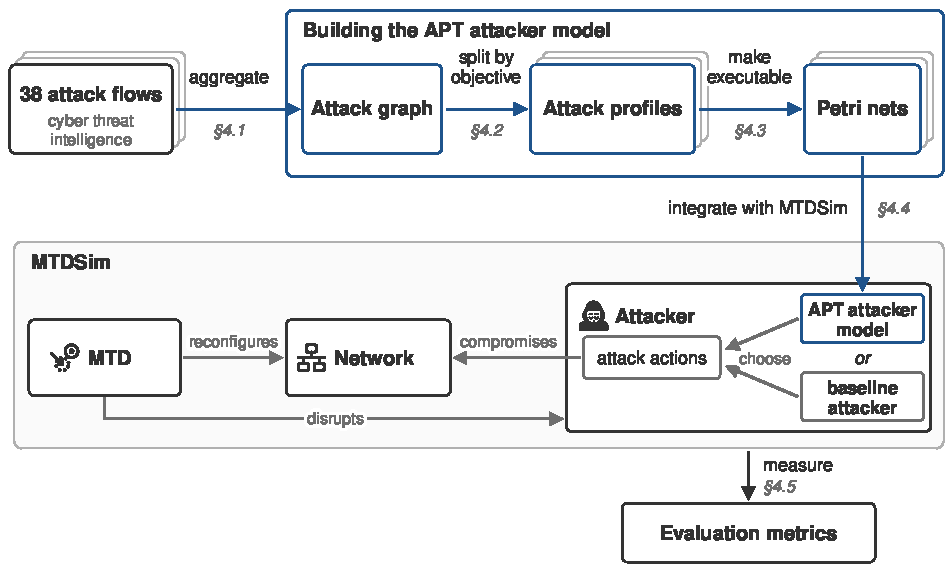
\includegraphics[width=\linewidth]{fig_4-0a_method_overview}
\end{column}
\begin{column}{0.37\textwidth}
\begin{itemize}
  \item \textbf{SQ1}: 38 attack flows $\to$ four \textbf{attack profiles} by objective
  \item \textbf{SQ2}: each runs as a Petri net
  \item \textbf{SQ3}: two attackers, same MTD
\end{itemize}
\vspace{2mm}
{\small
\begin{tabular}{@{}l l@{}}
c1 & stole data \\
c2 & impeded systems \\
c3 & both \\
c4 & neither \\
\end{tabular}}
\end{column}
\end{columns}
\end{frame}
\note[itemize]{
\item \textbf{3:30 to 4:45.} Three sub-questions, one pipeline: point left to right along the top row.
\item The 38 attack flows are analysts' hand-drawn graphs of reported intrusions, published by MITRE's Center for Threat-Informed Defense; the Volt Typhoon picture is one of the kind. Hand-drawn matters: automated extraction from report text is unreliable (best systems 80\,\% precision at 66\,\% recall on identifying techniques alone).
\item Aggregated into an attack graph over the 15 ATT\&CK tactics (what the attacker is trying to do: Initial Access, Lateral Movement, Exfiltration, \ldots). Tactics, not techniques: 88\,\% of technique-to-technique edges come from a single attack flow.
\item Split by two yes/no questions per attack flow: did it steal data, did it impede systems. c1 has 19 attack flows, c2 7, c3 7 (mostly ransomware), c4 5.
\item Transition: ``A graph does not run. Here is how it runs.''
}

% ============================================================================
% Ch4: Figure 4.5; Sections 4.3, 4.4.1 to 4.4.3; Figure 4.4(b).
\begin{frame}{A Petri net picks the next tactic; MTDSim carries it out}
\begin{columns}[T]
\begin{column}{0.62\textwidth}
  \centering
  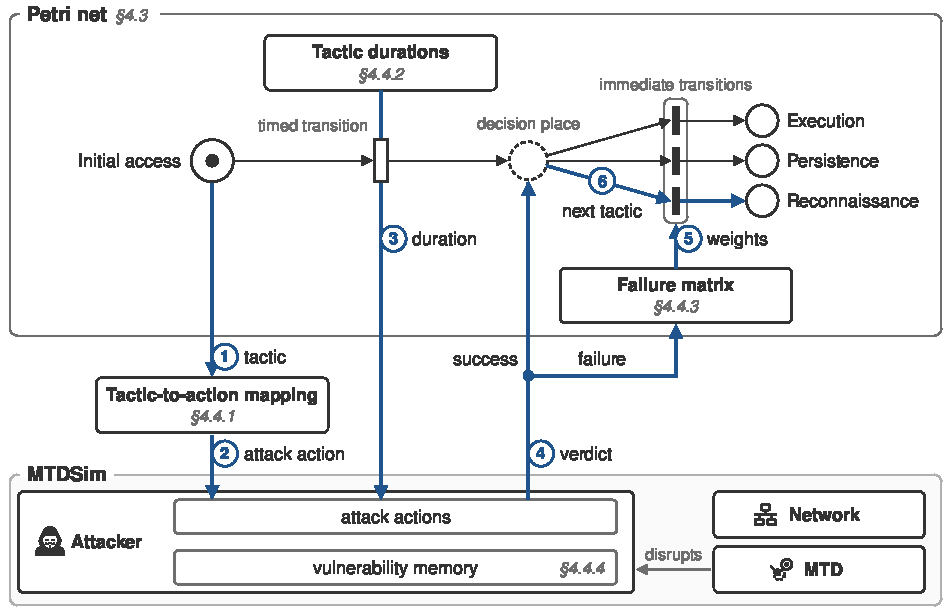
\includegraphics[width=\linewidth]{fig_4-4c_runtime_loop}
\end{column}
\begin{column}{0.35\textwidth}
\begin{itemize}
  \item Next tactic: drawn from the attack flows
  \item 7 of 15 tactics \textbf{unmapped}
  \item Timing and failures: declared
\end{itemize}
\end{column}
\end{columns}
\end{frame}
\note[itemize]{
\item \textbf{4:45 to 6:15.} Walk the loop once with your finger, steps 1 to 6: the token's tactic leaves the Petri net; the tactic-to-action mapping turns it into an attack action; it runs for the tactic duration; MTDSim returns success or failure; after a failure the failure matrix reweights; the token moves on.
\item Petri net: a generalised stochastic Petri net, the convention in MTD evaluation. Next tactic drawn in proportion to how many attack flows took that step, so runs differ.
\item Tactic-to-action mapping: 8 of 15 tactics run one of MTDSim's six attack actions. The other 7 (e.g.\ Exfiltration, Stealth) are unmapped and only take time. The ceiling: MTDSim's attack actions only find and compromise hosts, so the model steals no data. Say this plainly.
\item Threat reports record no timing and no failures. Tactic durations (up to 45\,s on average) and the failure matrix are declared before any result, then varied. Example: a failed Initial Access returns to Reconnaissance with weight 0.75, up from 0.06.
\item Likely questions: ``Why these durations?'' $\to$ backup \textit{Tactic durations}; ``Formal definition?'' $\to$ backup \textit{The Petri net}.
}

% ============================================================================
% Ch5: Table 5.1, Section 4.5.
\begin{frame}{Experiment: both attackers on the same 1\,000 networks}
\begin{columns}[T]
\begin{column}{0.52\textwidth}
\small
\begin{tabularx}{\linewidth}{@{}>{\bfseries}l >{\raggedright\arraybackslash}X@{}}
\toprule
Attacker & baseline; APT model, c1 to c4 \\
MTD & none; 7 mechanisms; 3 deployment strategies \\
Interval & 50 to 2\,000\,s \\
Seeds & 1\,000 per configuration \\
\bottomrule
\end{tabularx}
\end{column}
\begin{column}{0.45\textwidth}
\textbf{NCR}: share of hosts compromised\\[3mm]
\textbf{NCR reduction}\\[1mm]
$\displaystyle = 1 - \frac{\text{NCR under MTD}}{\text{NCR with no MTD}}$
\end{column}
\end{columns}
\end{frame}
\note[itemize]{
\item \textbf{6:15 to 7:00.} Keep this quick.
\item The design choice that matters: every configuration runs on the same 1\,000 seeds, so both attackers face the same 1\,000 networks. Differences come from the attacker, not the network. 1\,000 runs follows the recommendation for randomised algorithms (Arcuri and Briand).
\item MTD: none; each of the seven mechanisms alone; random and alternative rotation; MTDShield as released. Intervals 50, 100, 200, 500, 1\,000, 2\,000\,s.
\item Targeted scenario: a run ends at the first target host compromised, or at 15\,000\,s.
\item NCR, network compromise ratio (Zhang 2023). NCR reduction compares each attacker with its own runs with no MTD: 0 = no effect, 1 = nothing compromised.
\item MTD settings ranked by the Scott--Knott effect-size test; the two rankings compared with Spearman's $\rho$.
}

% ============================================================================
\section{Results}
% Ch5: Table 5.2, Figure 5.1(b), Section 5.2; Ch6 6.1.
\begin{frame}{No MTD: the APT attacker model acts more like an APT, but compromises less}
\small
\begin{tabularx}{\textwidth}{@{}>{\raggedright\arraybackslash}X >{\centering\arraybackslash}p{3.0cm} >{\centering\arraybackslash}p{2.4cm}@{}}
\toprule
 & APT attacker model & Baseline attacker \\
\midrule
Distinct openings (first 8 steps) & 179 to 947 & 3 \\
Attack actions per minute & 0.68 to 1.23 & 1.71 \\
Not flagged by a port-scan rule & 89 to 98\,\% & 82\,\% \\
\midrule
Runs reaching a target host (ASP) & 0.04 to 0.14 & 0.66 \\
Share of hosts compromised (NCR) & 0.15 to 0.21 & 0.50 \\
\bottomrule
\end{tabularx}
\normalsize
\takeaway{Same cause for both halves: its tactic durations and the order of its tactics.}
\end{frame}
\note[itemize]{
\item \textbf{7:00 to 8:15.} First, no MTD at all: does the model behave differently?
\item Row 1, choice of attack strategy: the baseline attacker's 1\,000 runs start the same way; the attack profiles' runs part ways by the second to fourth step. Ranges are over c1 to c4.
\item Rows 2 and 3, detection avoidance by proxy: it acts less often, and Snort's default port-scan rule (5 targets in 60\,s) would flag fewer of its attack actions. MTDSim has no IDS; say so.
\item Objective-specific behaviour (not on the slide): Exfiltration steps only in c1 and c3, Impact mostly in c2 and c3.
\item Bottom rows: it reaches a target in far fewer runs. Pre-empt the objection: ``Yes, with no MTD it is the weaker attacker. ASP and NCR alone would rate it weaker for exactly what makes it APT-like. With the baseline attacker's times it closes about two thirds of the gap.''
\item Transition: ``Two different attackers, the same networks. Now switch MTD on.''
\item Likely question: ``Isn't it just weaker?'' $\to$ backup \textit{Why it compromises less}.
}

% ============================================================================
% Ch5: Table 5.3 (200 s), Table F.4, Section 5.3.2.
\begin{frame}{Headline: the most effective MTD mechanism differs between the attackers}
\begin{columns}[T]
\begin{column}{0.56\textwidth}
\small
\begin{tabular}{@{}l >{\centering\arraybackslash}p{2.1cm} >{\centering\arraybackslash}p{2.1cm}@{}}
\toprule
NCR reduction at 200\,s & APT attacker model & Baseline attacker \\
\midrule
\multicolumn{3}{@{}l}{\textit{host layer}} \\
\quad IP shuffle & \textbf{96\,\% (1)} & 68\,\% (2) \\
\quad complete topology & \textbf{95\,\% (1)} & 42\,\% (3) \\
\quad host topology & \textbf{95\,\% (1)} & 38\,\% (3) \\
\multicolumn{3}{@{}l}{\textit{service layer}} \\
\quad service diversity & 36\,\% (4) & \textbf{92\,\% (1)} \\
\quad port shuffle & 20\,\% (6) & \textbf{91\,\% (1)} \\
\quad OS diversity & 7\,\% (7) & 68\,\% (2) \\
\multicolumn{3}{@{}l}{\textit{credentials}} \\
\quad user shuffle & $-10$\,\% (8) & $-5$\,\% (5) \\
\bottomrule
\end{tabular}\\[1mm]
{\scriptsize (rank) among all ten MTD settings}
\end{column}
\begin{column}{0.40\textwidth}
\begin{itemize}
  \item Rank 1 shares no mechanism
  \item Service diversity: 92 against 36\,\%
  \item Spearman's $\rho = 0.01$
\end{itemize}
\end{column}
\end{columns}
\end{frame}
\note[itemize]{
\item \textbf{8:15 to 9:45.} \textbf{This is the result. Slow down.}
\item Read the bold cells: against the APT attacker model, the host layer ranks first; against the baseline attacker, the service layer. Rank 1 shares no mechanism.
\item The one number: service diversity removes 92\,\% of the baseline attacker's NCR and 36\,\% of the APT attacker model's, on the same networks, with the same deployments.
\item $\rho = 0.01$: the two rankings are uncorrelated. Say ``do not agree'', not ``reversed''.
\item APT attacker model averaged over c1 to c4.
\item Only if asked: user shuffle is negative against the APT attacker model because it redraws accounts but leaves valid the ones the attacker holds, so each deployment is a fresh chance to log in.
\item Transition: ``Is that just the default interval?''
}

% ============================================================================
% Ch5: Figure 5.3 panels (a) and (b), redrawn per attacker from Table F.2; Figure 5.2 / Table F.1; Ch6 6.2.
\begin{frame}{The difference holds at every deployment interval}
\begin{columns}[T]
\begin{column}{0.58\textwidth}
\centering
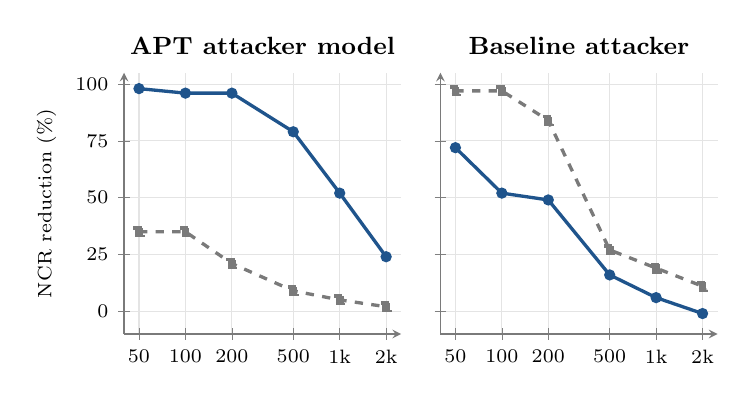
\begin{tikzpicture}
\begin{groupplot}[
  group style={group size=2 by 1, horizontal sep=5mm, y descriptions at=edge left},
  width=5.1cm, height=4.9cm, legend to name=layers,
  xmode=log, xmin=40, xmax=2500,
  xtick={50,100,200,500,1000,2000},
  xticklabels={50,100,200,500,1k,2k},
  ymin=-10, ymax=105, ytick={0,25,50,75,100},
  tick label style={font=\scriptsize},
  label style={font=\scriptsize},
  title style={font=\small\bfseries, yshift=-1mm},
  axis lines=left, axis line style={mid},
  grid=major, grid style={mid!20},
  legend style={font=\scriptsize, draw=none, legend columns=2, /tikz/every even column/.append style={column sep=4mm}},
]
\nextgroupplot[title={APT attacker model}, ylabel={NCR reduction (\%)}]
  \addplot[accent, very thick, mark=*, mark size=1.4pt] coordinates {(50,98)(100,96)(200,96)(500,79)(1000,52)(2000,24)};
  \addplot[mid, very thick, dashed, mark=square*, mark size=1.4pt] coordinates {(50,35)(100,35)(200,21)(500,9)(1000,5)(2000,2)};
\nextgroupplot[title={Baseline attacker}]
  \addplot[accent, very thick, mark=*, mark size=1.4pt] coordinates {(50,72)(100,52)(200,49)(500,16)(1000,6)(2000,-1)};
  \addplot[mid, very thick, dashed, mark=square*, mark size=1.4pt] coordinates {(50,97)(100,97)(200,84)(500,27)(1000,19)(2000,11)};
  \legend{host layer, service layer}
\end{groupplot}
\end{tikzpicture}\\[-0.5mm]
{\scriptsize Deployment interval (s, log scale)}\\[0.5mm]
\ref{layers}
\end{column}
\begin{column}{0.38\textwidth}
\textbf{Why} (measured at 2\,000\,s):
\begin{itemize}
  \item The service layer disrupts only port scans, exploits and brute force
  \item Blocks an attack action: 95\,\% baseline, 15\,\% APT model
  \item Host layer costs the APT model 242 to 324\,s
\end{itemize}
\end{column}
\end{columns}
\end{frame}
\note[itemize]{
\item \textbf{9:45 to 11:15.} Left: in each panel, which line is on top? APT attacker model: host layer, at every interval. Baseline attacker: service layer, at every interval. Each line is the mean over the layer's mechanisms.
\item The host layer keeps at least half of the APT attacker model's NCR off up to 1\,000\,s; the service layer does that for the baseline attacker only up to 200\,s.
\item Why: a deployment disrupts an attacker only if it lands while the attacker is doing what that layer breaks. The baseline attacker scans ports, exploits and brute-forces back to back; the APT attacker model sits mostly in unmapped tactics, which run no attack action.
\item A host-layer deployment costs the APT attacker model 242 to 324\,s: it has no host until its Petri net next reaches Lateral Movement. The baseline attacker loses none, because its procedure re-enumerates a host at once.
\item Say ``likely'': the tactic durations and the order of the tactics most likely explain it; no run separates the two.
\item Likely question: ``Does the host layer just stop it getting in?'' $\to$ backup \textit{Footholds under the host layer}. Answer: largely yes, at short intervals.
}

% ============================================================================
\section{So what}
% Ch6 6.4; Table F.2 (200 s); Appendix E.5.
\begin{frame}{The attacker model can decide which MTD looks best}
\begin{columns}[T]
\begin{column}{0.46\textwidth}
\centering
\small
\textbf{MTDShield}, learned against the baseline attacker\\[2mm]
\begin{tabular}{@{}l r r@{}}
\toprule
NCR reduction, 200\,s & Baseline & APT model \\
\midrule
MTDShield & \textbf{68\,\%} & 28\,\% \\
random deployment & 33\,\% & \textbf{75\,\%} \\
\bottomrule
\end{tabular}
\end{column}
\begin{column}{0.50\textwidth}
\begin{itemize}
  \item Test a learned strategy on an attacker it was not trained on
  \item Report a ranking with its attacker model
  \item Cost depends on the attacker model
\end{itemize}
\end{column}
\end{columns}
\takeaway{One simplified attacker cannot tell you how MTD performs against an APT.}
\end{frame}
\note[itemize]{
\item \textbf{11:15 to 12:45.} The ``so what'' for anyone who evaluates MTD.
\item MTDShield was trained and tested by Tay against the baseline attacker. It deploys service diversity in 70\,\% or more of its decisions against either attacker. Against the APT attacker model, random deployment does almost three times better. Most likely it learned the mechanism that disrupts its training attacker: a test in the training environment is a test on training data.
\item Fair to Tay: it runs as released, outside its training conditions; this bounds MTDShield as released, not retrained.
\item Recommendation 1: test a learned deployment strategy against an attacker model it was not trained on, beside random deployment over the same mechanisms.
\item Recommendation 2: report each ranking with the attacker model behind it; compare across studies only on a shared attacker model.
\item Recommendation 3, cost: to halve NCR, service diversity deploys every 1\,000\,s against the baseline attacker, but every 100\,s against the APT attacker model: ten times the overhead.
\item Optional question to the room: ``If you were choosing an MTD for a real network, which attacker model would you trust?''
}

% ============================================================================
\section{Conclusion}
% Ch6 6.5 (limitations; T1, T4, T5, T10, T11).
\begin{frame}{Limitations}
\begin{itemize}
  \item One simulator, one network size, no deployment cost
  \item Six attack actions: no data theft, no IDS
  \item Declared durations and failure matrix
  \item 38 attack flows
  \item Cause not isolated
\end{itemize}
\end{frame}
\note[itemize]{
\item \textbf{12:45 to 13:45.} State these yourself before anyone asks; examiners mark you for it.
\item One simulator: every claim holds in MTDSim, on its default 50-host network, with deployments that cost nothing.
\item MTDSim's six attack actions cap the model: 7 of 15 tactics unmapped, so no data theft, no impact, and no IDS to evade.
\item Declared values: tactic durations and failure matrix are judgement where threat reports are silent, fixed before any result. Only the 45\,s duration moves NCR much, and the ranking holds from a quarter to four times it.
\item Small corpus: 38 attack flows, 18 attributed to a known group; three attack profiles rest on 5 to 7.
\item Cause not isolated: tactic durations or the order of tactics. MTDSim's disruption rules were written for the baseline attacker; an APT holding a host through Command and Control might survive an IP shuffle. Both attackers meet the same rules, so the comparison is fair.
\item The headline does not say ``MTD fails against APTs'' or ``my attacker is the realistic one''. It says the ranking \emph{can depend} on the attacker model.
\item Likely question: ``How do you know the code does what you say?'' $\to$ backup \textit{Verification}.
}

% ============================================================================
% Ch7 drafting notes; Table 6.1; Section 7.2.
\begin{frame}{In MTDSim, the most effective MTD depends on the attacker model}
\begin{itemize}
  \item \textbf{Built}: an APT attacker model from 38 attack flows, runnable in MTDSim
  \item \textbf{Found}: host layer against it, service layer against the baseline attacker
  \item \textbf{Next}: richer attack actions, an IDS, deployment cost
\end{itemize}
\takeaway{Evaluate MTD against attacker models grounded in documented behaviour.}
\end{frame}
\note[itemize]{
\item \textbf{13:45 to 14:45.} Answer the research question in one sentence, then the two contributions. No new numbers; the audience has 92 against 36\,\%.
\item Contribution 1: the APT attacker model, which any MTDSim study can run in place of the baseline attacker. Two of the eight properties in full and three in part, against at most one in full for three recent models. A proof of concept, built, run and open-sourced; not a claim that it reproduces APT behaviour.
\item Contribution 2: the finding. At every deployment interval, the host layer disrupts the APT attacker model most and the service layer the baseline attacker.
\item Future work: attack actions for actions on objectives, and an IDS; separate the tactic durations from the order of tactics; deployment cost; other networks; MTDShield retrained against the APT attacker model.
\item Then move to the questions slide.
}

% ============================================================================
\begin{frame}[plain,noframenumbering]
\centering
\vfill
{\Huge\color{accent}\textbf{Questions?}}\\[8mm]
{\large How does MTD perform against APT attackers?}\\[2mm]
{\normalsize In MTDSim, it depends on which attacker it is tested against.}\\[10mm]
{\small\color{mid} Marc Labouchardiere \quad\textbullet\quad Supervisor: Dr Jin B. Hong}\\[1mm]
{\small\color{mid} Code and experiments: github.com/marc-la/MTDSim}
\vfill
\end{frame}
\note[itemize]{
\item Leave this up during questions.
\item Q\&A map: weaker attacker $\to$ \textit{Why it compromises less}; footholds $\to$ \textit{Footholds}; durations $\to$ \textit{Tactic durations}; components $\to$ \textit{Ablations}; per profile $\to$ \textit{Each attack profile}; scoring $\to$ \textit{Scoring}; Petri net $\to$ \textit{The Petri net}; MTDShield $\to$ \textit{MTDShield as run}; ASP $\to$ \textit{Disruption and ASP}; earlier numbers $\to$ \textit{Verification}.
}

% ============================================================================
% =========================== BACKUP SLIDES ==================================
% ============================================================================
\appendix
\setbeamertemplate{footline}{\hfill{\scriptsize\color{mid}Backup \insertframenumber}\hspace*{4mm}\vspace{2mm}}

% Ch6 6.1; Appendix G.3, Tables G.5 and G.6; T2.
\begin{frame}{Backup: why the APT attacker model compromises less with no MTD}
\begin{itemize}
  \item Unmapped tactics take 34 to 57\,\% of an attack profile's run, and 15 to 30\,\% of its attack actions fail because their preconditions are missing (e.g.\ exploit before scan port)
  \item Rerun with the baseline attacker's times in place of its tactic durations, same order of tactics: ASP rises from 0.09 to 0.45, against the baseline attacker's 0.66, closing 63\,\% of the gap
  \item The order of its tactics most likely accounts for the rest
  \item The rankings compare each attacker with its own NCR with no MTD, so the lower starting point is unlikely to decide which mechanism ranks first
\end{itemize}
\vfill{\scriptsize Dissertation Section 6.1, Appendix G.3, threat T2. Appendix G analyses were chosen after the results were seen (T9).}
\end{frame}

% Appendix G.4, Table G.7.
\begin{frame}{Backup: footholds under the host layer}
\begin{itemize}
  \item Under the three host-layer mechanisms at 50 to 200\,s, 70 to 89\,\% of the APT attacker model's runs compromise no host, against 3 to 20\,\% of the baseline attacker's
  \item With no MTD: 1\,\% and none
  \item So the host layer disrupts the APT attacker model mostly \emph{before} its first foothold: after a host-layer deployment it has no host until its Petri net next reaches Lateral Movement
  \item From 500\,s the share falls for both attackers, and the host layer still ranks first against the APT attacker model
\end{itemize}
\vfill{\scriptsize Dissertation Appendix G.4 (post hoc, T9); the claim stands on Chapter 5 without it.}
\end{frame}

% Appendix D.1, Tables D.3 and D.4.
\begin{frame}{Backup: are the declared tactic durations driving the result?}
\begin{columns}[T]
\begin{column}{0.48\textwidth}
\small
\begin{tabular}{@{}l r r r@{}}
\toprule
Mean duration (band) & low & declared & high \\
\midrule
4.5\,s (2.25 to 9) & 0.165 & 0.163 & 0.159 \\
35\,s (17.5 to 70) & 0.172 & 0.163 & 0.145 \\
36\,s (18 to 72) & 0.170 & 0.163 & 0.148 \\
45\,s (11.25 to 180) & \textbf{0.267} & 0.163 & \textbf{0.059} \\
\bottomrule
\end{tabular}\\[1mm]
{\scriptsize NCR with no MTD, each value moved alone, 400 runs per cell.}
\end{column}
\begin{column}{0.48\textwidth}
\begin{itemize}
  \item Bands fixed before the run; one value moved at a time
  \item Only the 45\,s (Persistence, Stealth, Command and Control) moves NCR much: Command and Control is the only tactic that finds new hosts
  \item At a quarter and four times the 45\,s, rank 1 still shares no mechanism with the baseline attacker's, and the host layer still ranks above the service layer ($\rho = 0.03$ and $-0.03$)
  \item Untested: interactions between values
\end{itemize}
\end{column}
\end{columns}
\vfill{\scriptsize Dissertation Appendix D.1, threat T4.}
\end{frame}

% Section 5.4, Table 5.4.
\begin{frame}{Backup: what each component of the APT attacker model changes}
\centering
\small
\begin{tabular}{@{}l l r r r@{}}
\toprule
Component removed & MTD & NCR with & without & Cohen's $d$ \\
\midrule
Attack profiles (use the whole attack graph) & no MTD & 0.171 & 0.189 & \textbf{$-0.28$} \\
 & IP shuffle, 200\,s & 0.007 & 0.013 & \textbf{$-0.47$} \\
 & OS diversity, 200\,s & 0.159 & 0.174 & \textbf{$-0.26$} \\
\midrule
Failure matrix & no MTD & 0.171 & 0.167 & $+0.07$ \\
 & IP shuffle, 200\,s & 0.007 & 0.006 & $+0.13$ \\
\midrule
Vulnerability memory & no MTD & 0.171 & 0.169 & $+0.04$ \\
 & service diversity, 200\,s & 0.109 & 0.106 & $+0.07$ \\
\bottomrule
\end{tabular}\\[2mm]
\raggedright
\begin{itemize}
  \item Bold: not negligible ($|d| > 0.2$). The failure matrix changes \emph{where} the attacker goes after a failure (back to Reconnaissance 76 to 83\,\% vs 8 to 10\,\%), not what it achieves
  \item Without the attack profiles, the same three host-layer mechanisms still rank first
\end{itemize}
\end{frame}

% Figure 5.4.
\begin{frame}{Backup: each attack profile against the baseline attacker}
\centering
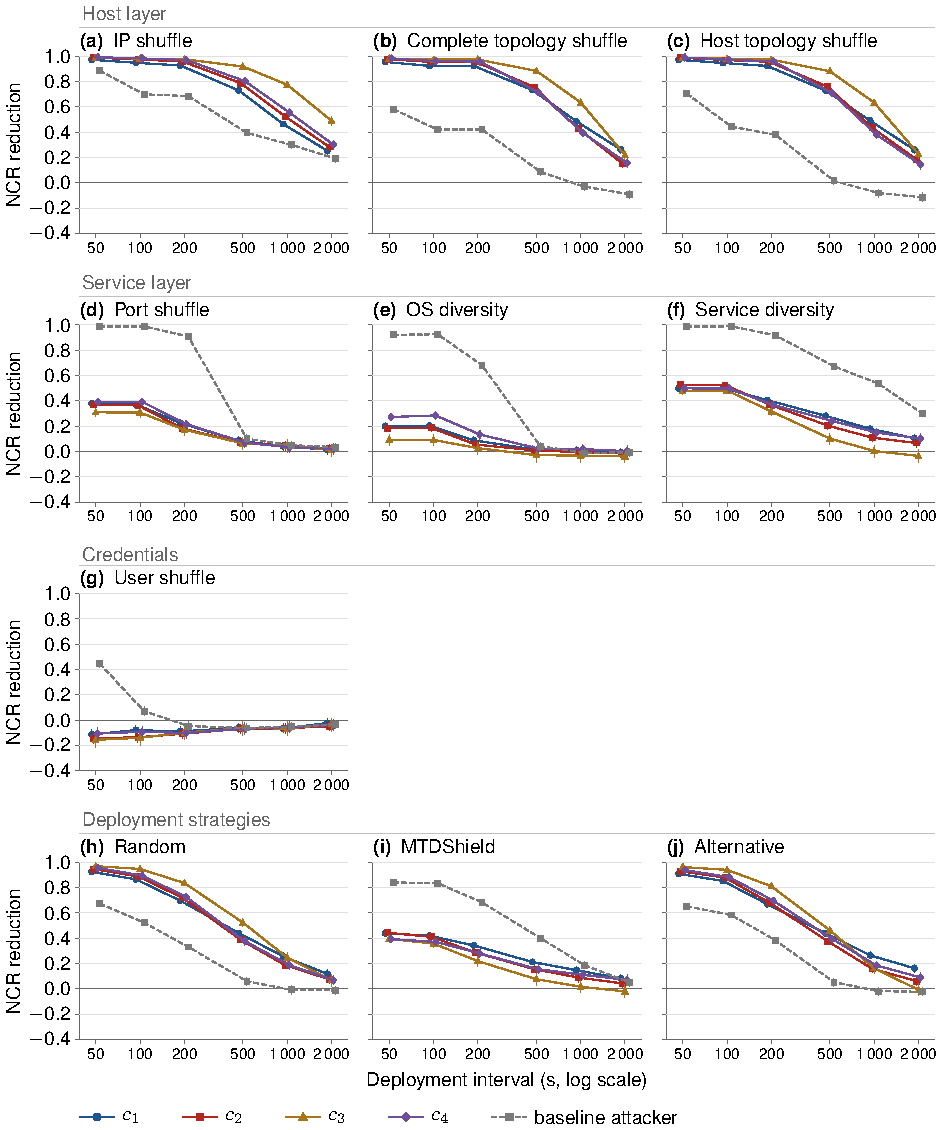
\includegraphics[height=0.80\textheight]{fig_5-3-3b_interval_mechanisms}\\
{\scriptsize At 50 to 200\,s the four attack profiles differ from one another less than the baseline attacker differs from the nearest of them (dissertation Figure 5.4).}
\end{frame}

% Table 6.1, Section 3.3.2, T7.
\begin{frame}{Backup: scoring the eight properties}
\centering
\small
\begin{tabular}{@{}l c c c c c c c c@{}}
\toprule
 & 1 & 2 & 3 & 4 & 5 & 6 & 7 & 8 \\
Attacker model & Pers. & Obj. & Strat. & Adapt. & Detect. & Cost & Learn. & Deploy. \\
\midrule
Baseline attacker (2023) & \yes & \no & part & part & \no & \no & \no & \no \\
Masud et al.\ (2025) & part & \no & \no & \no & \no & \no & \no & \no \\
Kim et al.\ (2026) & part & \no & \no & \no & part & \no & \no & \no \\
\textbf{APT attacker model} & \yes & part & \yes & part & part & \no & \no & \no \\
\bottomrule
\end{tabular}\\[2mm]
\raggedright
\begin{itemize}
  \item Each property split into predicates; \yes{} = every predicate true of the model's own behaviour; part = a behaviour predicate true, but set by a fixed rule or assumed
  \item One scorer, checked by blind scoring with language models (dissertation Appendix B)
  \item Adaptivity is in part because the failure matrix is a fixed rule of mine; detection avoidance in part because MTDSim has no IDS
\end{itemize}
\end{frame}

% Section 4.3, Equations 4.2 and 4.4, Figure 4.4.
\begin{frame}{Backup: the Petri net}
\begin{columns}[T]
\begin{column}{0.52\textwidth}
\centering
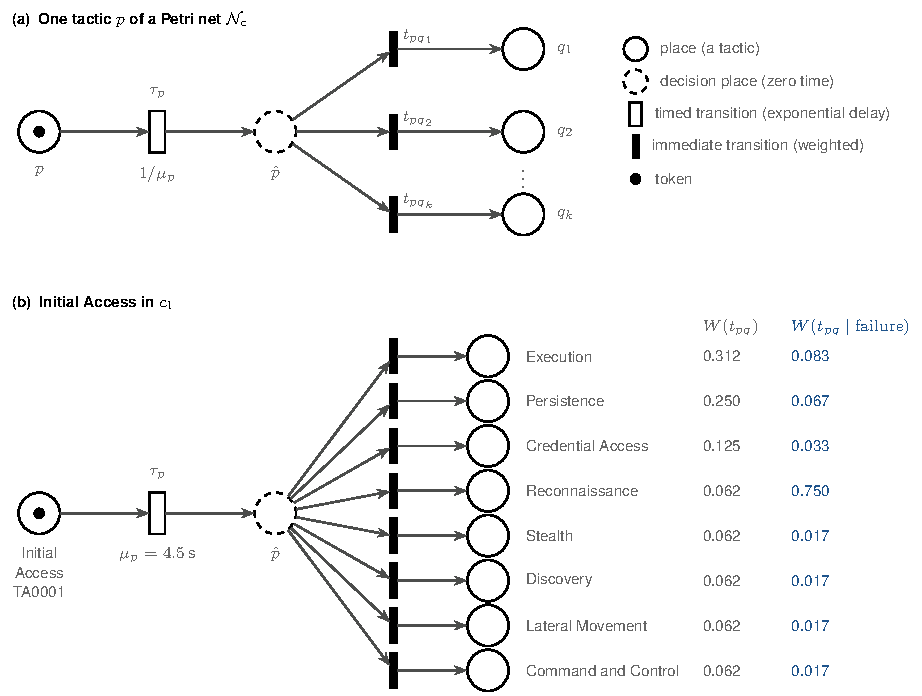
\includegraphics[width=\linewidth]{fig_4-3a_gspn_gadget}
\end{column}
\begin{column}{0.45\textwidth}
\small
Generalised stochastic Petri net \src{Ajmone Marsan 1995}, extended with the failure matrix $F$:
\[(P, T, I, O, W, M_0, F)\]
Base weight of the move from tactic $p$ to $q$:
\[W(t_{pq}) = \frac{n(p,q)}{\sum_{q'} n(p,q')}\]
with $n(p,q)$ the attack flows that draw $p \to q$. After a failed attack action:
\[W(t_{pq}\mid\text{failure}) = \frac{W(t_{pq})\,F(p,q)}{\sum_{q'} W(t_{pq'})\,F(p,q')}\]
One token, starting on Reconnaissance.
\end{column}
\end{columns}
\end{frame}

% Table 4.2, Figure 4.6.
\begin{frame}{Backup: tactic durations and the tactic-to-action mapping}
\begin{columns}[T]
\begin{column}{0.50\textwidth}
\small
\begin{tabular}{@{}>{\raggedright\arraybackslash}p{0.72\linewidth} r@{}}
\toprule
Tactics & Mean (s) \\
\midrule
Initial Access, Privilege Escalation, Credential Access, Lateral Movement {\scriptsize(MTDSim's exploit)} & 4.5 \\
Reconnaissance, Discovery {\scriptsize(MTDSim's three scans)} & 35 \\
Persistence, Stealth, Command and Control & 45 \\
Collection, Exfiltration, Impact & 36 \\
Execution, Defense Impairment & 22.5 \\
Resource Development & 0 \\
\bottomrule
\end{tabular}\\[1mm]
{\scriptsize Last four rows: judgement, kept on the baseline attacker's time scale and under the 200\,s default interval.}
\end{column}
\begin{column}{0.46\textwidth}
\centering
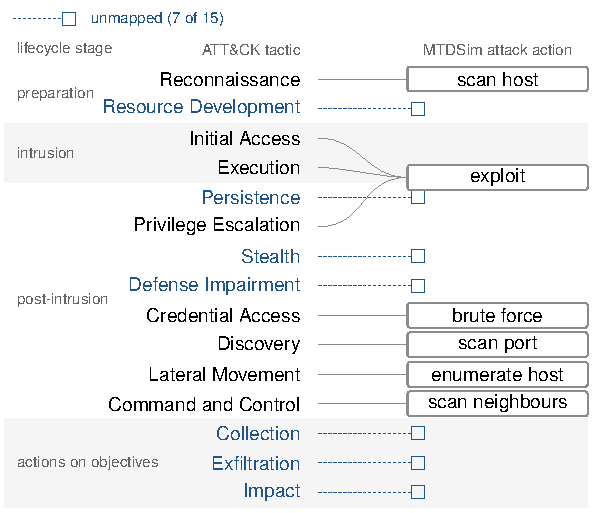
\includegraphics[width=\linewidth]{fig_4-4a_controller_mapping}
\end{column}
\end{columns}
\end{frame}

% Appendix E.4 and E.5.
\begin{frame}{Backup: MTDShield as run}
\begin{itemize}
  \item Run as released by Tay (2024); correcting the release would make it my agent, not Tay's
  \item Trained at one deployment interval, against the baseline attacker, on 100-host networks
  \item Known limits of the release: published scores produced with exploration at one; four evaluation inputs read as zero; ``do nothing'' never a learning target
  \item Its detection input reads an unmapped tactic as ``nothing detected''
  \item So the result bounds MTDShield \emph{as released}, not MTDShield retrained against the APT attacker model
\end{itemize}
\vfill{\scriptsize Dissertation Appendix E, threat T12.}
\end{frame}

% Figure 5.2; Appendix F.1, Table F.3.
\begin{frame}{Backup: disruption per MTD deployment, and ASP}
\begin{columns}[T]
\begin{column}{0.58\textwidth}
\centering
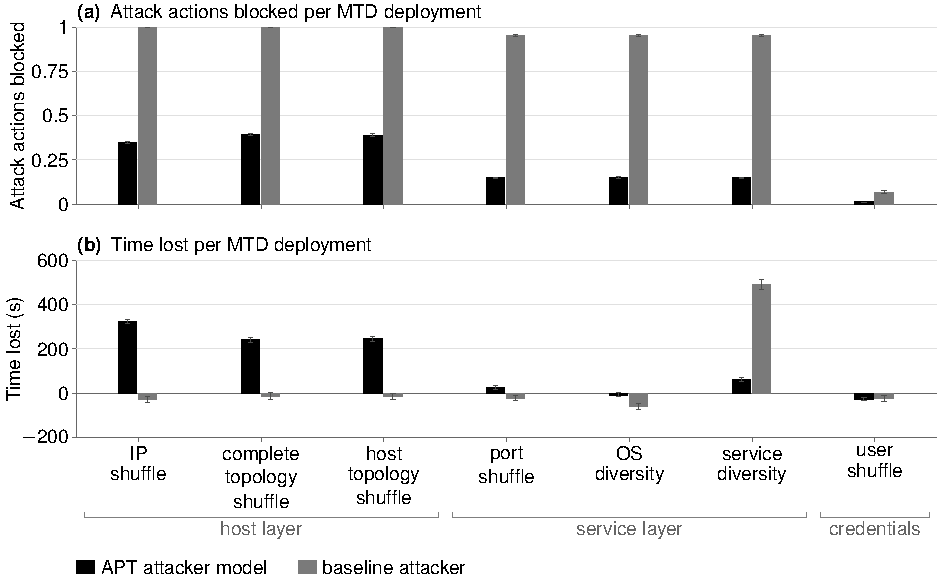
\includegraphics[width=\linewidth]{fig_5-2-2a_disruption_response}
\end{column}
\begin{column}{0.39\textwidth}
\begin{itemize}
  \item Measured at 2\,000\,s, because the next deployment caps time lost at the interval
  \item The baseline attacker's time lost is at or below zero after the first deployment: sent back to scan host, it gets a second attempt at its first host, as MTDSim intends
  \item On ASP reduction the layer order also holds against each attacker (Table F.3)
\end{itemize}
\end{column}
\end{columns}
\end{frame}

% T3.
\begin{frame}{Backup: verification, and why no comparison with earlier MTDSim numbers}
\begin{itemize}
  \item An event tracer replays any run step by step, across Petri net, attacker and MTD
  \item MTDSim's code audited against what its papers describe; unit tests of the Petri net and the simulator
  \item Fixed seeds reproduce every run exactly
  \item Defects found in MTDSim were repaired before the evaluation, so results are not compared numerically with Zhang (2023) or Tay (2024)
\end{itemize}
\vfill{\scriptsize Dissertation threat T3.}
\end{frame}

\begin{frame}{References}
\scriptsize
\begin{itemize}
  \item[] A.~Alshamrani et al., ``A survey on advanced persistent threats,'' \emph{IEEE Commun.\ Surveys Tuts.}, 21(2), 2019.
  \item[] M.~Ajmone Marsan et al., \emph{Modelling with Generalized Stochastic Petri Nets}, Wiley, 1995.
  \item[] A.~Brown, T.-W.~Lee and J.~B.~Hong, ``Evaluating moving target defenses against realistic attack scenarios,'' EnCyCriS, 2023.
  \item[] Center for Threat-Informed Defense, ``Attack Flow,'' MITRE, v3.2.0, 2025.
  \item[] J.-H.~Cho et al., ``Toward proactive, adaptive defense: A survey on moving target defense,'' \emph{IEEE Commun.\ Surveys Tuts.}, 22(1), 2020.
  \item[] CISA et al., ``PRC state-sponsored actors compromise and maintain persistent access to U.S.\ critical infrastructure,'' Advisory AA24-038A, 2024.
  \item[] {\L}.~Jalowski et al., ``Rethinking the security assurances of MTD: A gap analysis for network defense,'' \emph{Future Internet}, 18(2), 2026.
  \item[] M.~Kim et al., ``MTD in depth: Multi-phased moving target defense techniques against cyber-attacks based on cyber kill chain,'' \emph{FGCS}, 181, 2026.
  \item[] M.~T.~Masud et al., ``Vulnerability defence using hybrid moving target defence in Internet of Things systems,'' \emph{Computers \& Security}, 153, 2025.
  \item[] Joint Task Force, ``Managing information security risk,'' NIST SP 800-39, 2011.
  \item[] C.~Tantithamthavorn et al., ``An empirical comparison of model validation techniques for defect prediction models,'' \emph{IEEE TSE}, 43(1), 2017.
  \item[] J.~K.~Tay, ``Using artificial intelligence to automate the deployment of moving target defence operations,'' UWA research report, 2024.
  \item[] W.~Zhang, ``Evaluating multiple moving target defence in the time domain,'' Master's thesis, UWA, 2023.
\end{itemize}
\end{frame}

\end{document}
"  (twice)
% Slides carry prompts only; what to say is in each frame's \note.
% Every number on a slide is taken from the dissertation; the table or
% figure it comes from is named in the frame's comment.
\documentclass[aspectratio=169,11pt]{beamer}

\usepackage[T1]{fontenc}
\usepackage[scaled=0.92]{helvet}   % the figures' face
\usepackage{booktabs}
\usepackage{array}
\usepackage{tabularx}
\usepackage{pifont}
\usepackage{pgfplots}
\pgfplotsset{compat=1.17}
\usepgfplotslibrary{groupplots}
\usepackage{appendixnumberbeamer}   % "n / 12" counts the main slides only
\graphicspath{{../figures/}}

\ifdefined\withnotes
  \setbeameroption{show notes}
\fi

% --- look: plain, legible, one accent ---------------------------------------
\definecolor{accent}{RGB}{31,84,140}
\definecolor{mid}{RGB}{122,122,122}
\setbeamertemplate{navigation symbols}{}
\setbeamercolor{frametitle}{fg=accent}
\setbeamerfont{frametitle}{size=\large,series=\bfseries}
\setbeamercolor{structure}{fg=accent}
\setbeamertemplate{itemize items}{\color{accent}\textbullet}
\setbeamertemplate{itemize subitem}{\color{mid}--}
\setbeamersize{text margin left=8mm,text margin right=8mm}

% --- footer: the talk's timeline (sections, one dot per slide) + n / 12 -----
\useoutertheme[subsection=false]{miniframes}
\setbeamertemplate{headline}{}
\setbeamertemplate{mini frames}[default]
\setbeamercolor{section in head/foot}{fg=accent}
\setbeamercolor{mini frame}{fg=accent}
\setbeamerfont{section in head/foot}{size=\scriptsize}
\setbeamertemplate{footline}{%
  \begin{beamercolorbox}[wd=\paperwidth,ht=4mm,dp=3.6mm]{section in head/foot}%
    \hspace*{2mm}\insertnavigation{0.82\paperwidth}\hfill
    {\scriptsize\color{mid}\insertframenumber\,/\,\inserttotalframenumber}\hspace*{4mm}%
  \end{beamercolorbox}}

\newcommand{\src}[1]{{\scriptsize\color{mid}[#1]}}
\newcommand{\yes}{\ding{51}}
\newcommand{\no}{{\color{mid}\ding{55}}}
\newcommand{\takeaway}[1]{\vfill{\color{accent}\rule{\linewidth}{0.4pt}}\\[1mm]#1\vspace{1mm}}

\title{Evaluating moving target defence against advanced persistent threat attackers modelled on documented intrusion campaigns}
\author{Marc Labouchardiere\\[1mm]{\small Supervisor: Dr Jin B. Hong}}
\institute{\small Honours seminar, The University of Western Australia}
\date{\small 2026}

\begin{document}

% ============================================================================
\begin{frame}[plain,noframenumbering]
  \titlepage
\end{frame}
\note[itemize]{
\item \textbf{0:00 to 0:15.} Name, supervisor.
\item One line: ``I test whether MTD's measured effectiveness survives a change of attacker.''
\item The footer is the talk's timeline: six parts, one dot per slide.
}

% ============================================================================
\section{Motivation}
% Ch1; ch3 3.1.1 and 3.1.3; Figure 3.2.
\begin{frame}{MTD is proposed against APT attackers, but rarely tested against one}
\begin{columns}[T]
\begin{column}{0.44\textwidth}
\begin{itemize}
  \item \textbf{Advanced persistent threat (APT)}: one target, months to years
  \item Volt Typhoon: five years inside US infrastructure \src{CISA 2024}
  \item \textbf{Moving target defence (MTD)}: keep the network moving
  \item Tested against simple, scripted attackers
\end{itemize}
\end{column}
\begin{column}{0.53\textwidth}
  \centering
  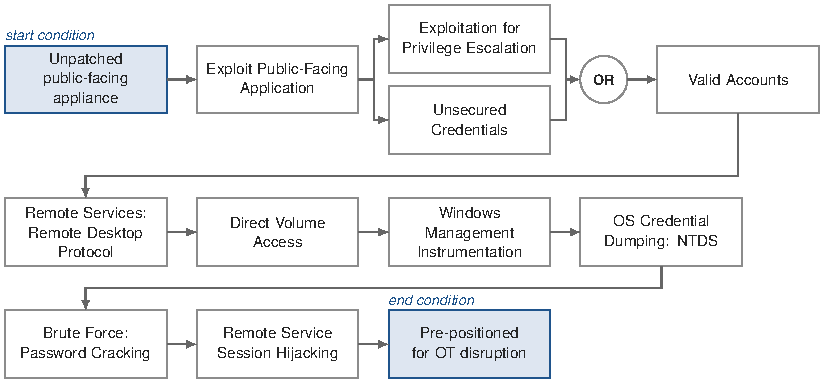
\includegraphics[width=\linewidth]{fig_3-1-3a_attack_flow_volt_typhoon}\\[1mm]
  {\scriptsize Volt Typhoon's intrusion as an \textbf{attack flow}}
\end{column}
\end{columns}
\takeaway{\textbf{Research question:} How does MTD perform against APT attackers?}
\end{frame}
\note[itemize]{
\item \textbf{0:15 to 1:30.} APT: a well-resourced attacker, often state-sponsored, pursuing one objective against one target over months or years (Alshamrani 2019). Espionage intrusions go undetected for a median of 122 days (Mandiant 2026).
\item Volt Typhoon held footholds in US critical infrastructure for at least five years, signing in with stolen valid accounts. Its reconnaissance stayed valid because the networks never changed.
\item MTD: change addresses, topology, software and credentials on a schedule, so what the attacker learned goes out of date even if it is never detected (Cho 2020).
\item Point at the attack flow: ``This is what a threat report gives us: the steps, in order, drawn by an analyst. It is the raw material of my attacker.''
\item The gap: MTD is proposed against APTs, but tested in simulation against attackers far simpler than an APT (Jalowski 2026). Read the research question aloud.
\item Transition: ``To test that, I need an MTD simulator and an attacker.''
}

% ============================================================================
\section{Previous work}
% Ch2: Figure 2.2, Table 2.1, Section 2.2.3.
\begin{frame}{MTDSim: seven MTD mechanisms, one scripted attacker}
\begin{columns}[T]
\begin{column}{0.44\textwidth}
\begin{itemize}
  \item \textbf{MTDSim} \src{Brown 2023; Zhang 2023; Tay 2024}
  \item \textbf{Host layer}: where hosts are
  \item \textbf{Service layer}: what runs on them
  \item \textbf{Baseline attacker}: six \textbf{attack actions}, fixed order
\end{itemize}
\end{column}
\begin{column}{0.53\textwidth}
  \centering
  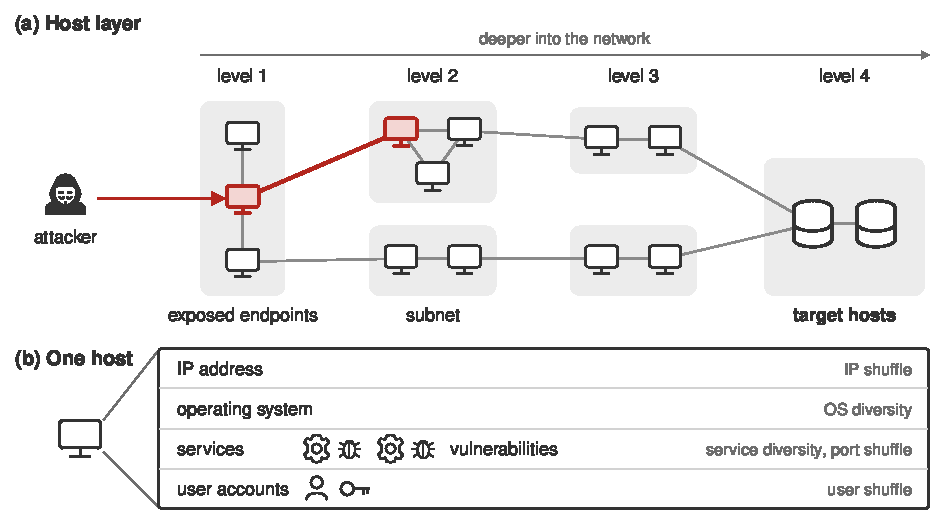
\includegraphics[width=\linewidth]{fig_2-2-1a_network_model}
\end{column}
\end{columns}
\end{frame}
\note[itemize]{
\item \textbf{1:30 to 2:30.} The work I inherit: Brown built MTDSim at UWA, Zhang added simulated time, Tay added MTDShield, a reinforcement-learning agent that picks which mechanism to deploy.
\item Panel (a): 50 hosts in four levels; the attacker enters at an exposed endpoint and works towards the target hosts.
\item Panel (b): each part of a host has a mechanism that moves it. Seven MTD mechanisms, one deployed every deployment interval (200\,s by default).
\item \textbf{The two layers the results hinge on}: host layer = IP shuffle and two topology shuffles; service layer = port shuffle, OS diversity, service diversity. Plus user shuffle on credentials.
\item Baseline attacker: scan host, enumerate host, scan port, exploit, brute force, scan neighbours; the same order every run.
\item Transition: ``Is a fixed procedure a fair stand-in for an APT?''
}

% ============================================================================
% Ch3: Tables 3.2 and 3.3.
\begin{frame}{Recent MTD attacker models lack most APT properties}
\centering
\small
\begin{tabular}{@{}l l c c c@{}}
\toprule
 & Property & Baseline attacker & Masud et al. & Kim et al. \\
 & & {\scriptsize 2023} & {\scriptsize 2025} & {\scriptsize 2026} \\
\midrule
1 & Campaign persistence & \yes & part & part \\
2 & Objective-specific behaviour & \no & \no & \no \\
3 & Choice of attack strategy & part & \no & \no \\
4 & Adaptivity to MTD disruption & part & \no & \no \\
5 & Detection avoidance & \no & \no & part \\
6 & Cost--benefit reasoning & \no & \no & \no \\
7 & Learning from past deployments & \no & \no & \no \\
8 & Deployment-strategy awareness & \no & \no & \no \\
\bottomrule
\end{tabular}\\[1mm]
{\scriptsize 1, 2, 4, 5: the APT definition \src{Alshamrani 2019; NIST 2011}. 3, 6, 7, 8: two MTD surveys \src{Cho 2020; Jalowski 2026}.}
\takeaway{\textbf{Gap}: how MTD performs against APT attackers is unmeasured.}
\end{frame}
\note[itemize]{
\item \textbf{2:30 to 3:30.} Eight properties: four from what an APT is, four that two MTD surveys say attacker models lack. Jalowski et al. call the attacker model ``the most glaring flaw in the MTD literature''.
\item I scored the baseline attacker and the two most recent MTD evaluations that describe their attacker in Kill Chain or ATT\&CK terms, the ones I expected to do best.
\item Read the result: at most one property in full, campaign persistence, only for the baseline attacker. None has objective-specific behaviour.
\item I targeted three: objective-specific behaviour, choice of attack strategy, adaptivity.
\item Likely question: ``How did you score them?'' $\to$ backup \textit{Scoring the eight properties}.
}

% ============================================================================
\section{Method}
% Ch4: Figure 4.1, Section 4.1, Table 4.1.
\begin{frame}{Build an APT attacker model from threat reports; run it in MTDSim}
\begin{columns}[T]
\begin{column}{0.60\textwidth}
  \centering
  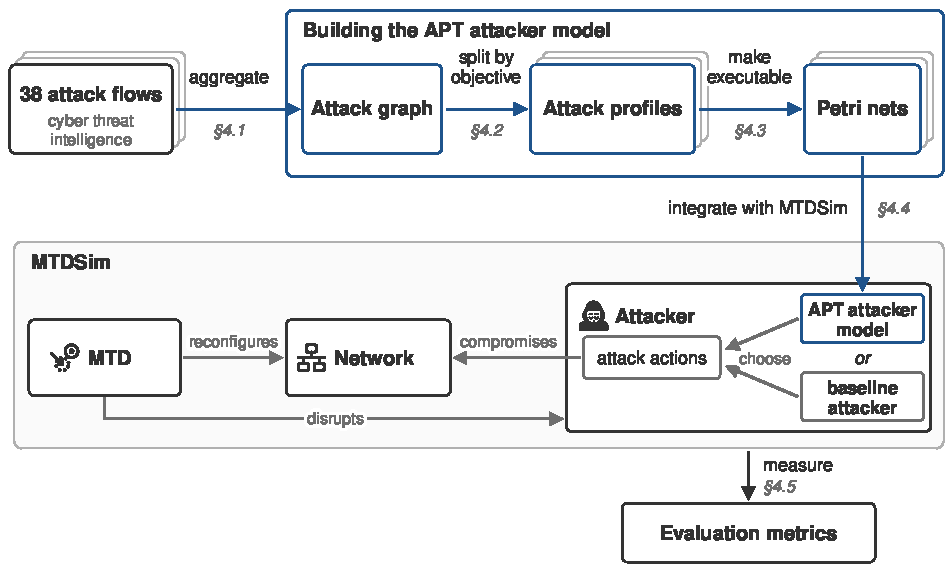
\includegraphics[width=\linewidth]{fig_4-0a_method_overview}
\end{column}
\begin{column}{0.37\textwidth}
\begin{itemize}
  \item \textbf{SQ1}: 38 attack flows $\to$ four \textbf{attack profiles} by objective
  \item \textbf{SQ2}: each runs as a Petri net
  \item \textbf{SQ3}: two attackers, same MTD
\end{itemize}
\vspace{2mm}
{\small
\begin{tabular}{@{}l l@{}}
c1 & stole data \\
c2 & impeded systems \\
c3 & both \\
c4 & neither \\
\end{tabular}}
\end{column}
\end{columns}
\end{frame}
\note[itemize]{
\item \textbf{3:30 to 4:45.} Three sub-questions, one pipeline: point left to right along the top row.
\item The 38 attack flows are analysts' hand-drawn graphs of reported intrusions, published by MITRE's Center for Threat-Informed Defense; the Volt Typhoon picture is one of the kind. Hand-drawn matters: automated extraction from report text is unreliable (best systems 80\,\% precision at 66\,\% recall on identifying techniques alone).
\item Aggregated into an attack graph over the 15 ATT\&CK tactics (what the attacker is trying to do: Initial Access, Lateral Movement, Exfiltration, \ldots). Tactics, not techniques: 88\,\% of technique-to-technique edges come from a single attack flow.
\item Split by two yes/no questions per attack flow: did it steal data, did it impede systems. c1 has 19 attack flows, c2 7, c3 7 (mostly ransomware), c4 5.
\item Transition: ``A graph does not run. Here is how it runs.''
}

% ============================================================================
% Ch4: Figure 4.5; Sections 4.3, 4.4.1 to 4.4.3; Figure 4.4(b).
\begin{frame}{A Petri net picks the next tactic; MTDSim carries it out}
\begin{columns}[T]
\begin{column}{0.62\textwidth}
  \centering
  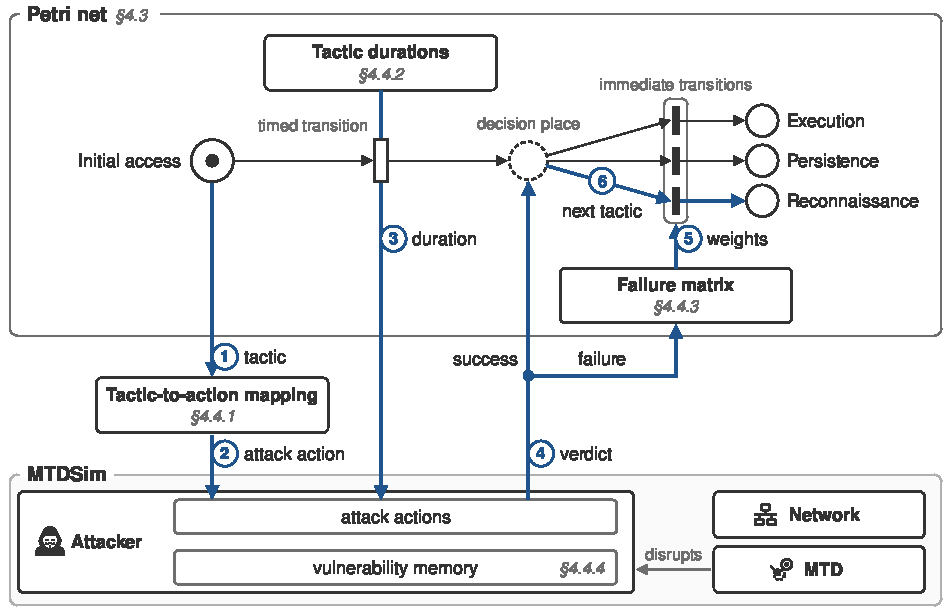
\includegraphics[width=\linewidth]{fig_4-4c_runtime_loop}
\end{column}
\begin{column}{0.35\textwidth}
\begin{itemize}
  \item Next tactic: drawn from the attack flows
  \item 7 of 15 tactics \textbf{unmapped}
  \item Timing and failures: declared
\end{itemize}
\end{column}
\end{columns}
\end{frame}
\note[itemize]{
\item \textbf{4:45 to 6:15.} Walk the loop once with your finger, steps 1 to 6: the token's tactic leaves the Petri net; the tactic-to-action mapping turns it into an attack action; it runs for the tactic duration; MTDSim returns success or failure; after a failure the failure matrix reweights; the token moves on.
\item Petri net: a generalised stochastic Petri net, the convention in MTD evaluation. Next tactic drawn in proportion to how many attack flows took that step, so runs differ.
\item Tactic-to-action mapping: 8 of 15 tactics run one of MTDSim's six attack actions. The other 7 (e.g.\ Exfiltration, Stealth) are unmapped and only take time. The ceiling: MTDSim's attack actions only find and compromise hosts, so the model steals no data. Say this plainly.
\item Threat reports record no timing and no failures. Tactic durations (up to 45\,s on average) and the failure matrix are declared before any result, then varied. Example: a failed Initial Access returns to Reconnaissance with weight 0.75, up from 0.06.
\item Likely questions: ``Why these durations?'' $\to$ backup \textit{Tactic durations}; ``Formal definition?'' $\to$ backup \textit{The Petri net}.
}

% ============================================================================
% Ch5: Table 5.1, Section 4.5.
\begin{frame}{Experiment: both attackers on the same 1\,000 networks}
\begin{columns}[T]
\begin{column}{0.52\textwidth}
\small
\begin{tabularx}{\linewidth}{@{}>{\bfseries}l >{\raggedright\arraybackslash}X@{}}
\toprule
Attacker & baseline; APT model, c1 to c4 \\
MTD & none; 7 mechanisms; 3 deployment strategies \\
Interval & 50 to 2\,000\,s \\
Seeds & 1\,000 per configuration \\
\bottomrule
\end{tabularx}
\end{column}
\begin{column}{0.45\textwidth}
\textbf{NCR}: share of hosts compromised\\[3mm]
\textbf{NCR reduction}\\[1mm]
$\displaystyle = 1 - \frac{\text{NCR under MTD}}{\text{NCR with no MTD}}$
\end{column}
\end{columns}
\end{frame}
\note[itemize]{
\item \textbf{6:15 to 7:00.} Keep this quick.
\item The design choice that matters: every configuration runs on the same 1\,000 seeds, so both attackers face the same 1\,000 networks. Differences come from the attacker, not the network. 1\,000 runs follows the recommendation for randomised algorithms (Arcuri and Briand).
\item MTD: none; each of the seven mechanisms alone; random and alternative rotation; MTDShield as released. Intervals 50, 100, 200, 500, 1\,000, 2\,000\,s.
\item Targeted scenario: a run ends at the first target host compromised, or at 15\,000\,s.
\item NCR, network compromise ratio (Zhang 2023). NCR reduction compares each attacker with its own runs with no MTD: 0 = no effect, 1 = nothing compromised.
\item MTD settings ranked by the Scott--Knott effect-size test; the two rankings compared with Spearman's $\rho$.
}

% ============================================================================
\section{Results}
% Ch5: Table 5.2, Figure 5.1(b), Section 5.2; Ch6 6.1.
\begin{frame}{No MTD: the APT attacker model acts more like an APT, but compromises less}
\small
\begin{tabularx}{\textwidth}{@{}>{\raggedright\arraybackslash}X >{\centering\arraybackslash}p{3.0cm} >{\centering\arraybackslash}p{2.4cm}@{}}
\toprule
 & APT attacker model & Baseline attacker \\
\midrule
Distinct openings (first 8 steps) & 179 to 947 & 3 \\
Attack actions per minute & 0.68 to 1.23 & 1.71 \\
Not flagged by a port-scan rule & 89 to 98\,\% & 82\,\% \\
\midrule
Runs reaching a target host (ASP) & 0.04 to 0.14 & 0.66 \\
Share of hosts compromised (NCR) & 0.15 to 0.21 & 0.50 \\
\bottomrule
\end{tabularx}
\normalsize
\takeaway{Same cause for both halves: its tactic durations and the order of its tactics.}
\end{frame}
\note[itemize]{
\item \textbf{7:00 to 8:15.} First, no MTD at all: does the model behave differently?
\item Row 1, choice of attack strategy: the baseline attacker's 1\,000 runs start the same way; the attack profiles' runs part ways by the second to fourth step. Ranges are over c1 to c4.
\item Rows 2 and 3, detection avoidance by proxy: it acts less often, and Snort's default port-scan rule (5 targets in 60\,s) would flag fewer of its attack actions. MTDSim has no IDS; say so.
\item Objective-specific behaviour (not on the slide): Exfiltration steps only in c1 and c3, Impact mostly in c2 and c3.
\item Bottom rows: it reaches a target in far fewer runs. Pre-empt the objection: ``Yes, with no MTD it is the weaker attacker. ASP and NCR alone would rate it weaker for exactly what makes it APT-like. With the baseline attacker's times it closes about two thirds of the gap.''
\item Transition: ``Two different attackers, the same networks. Now switch MTD on.''
\item Likely question: ``Isn't it just weaker?'' $\to$ backup \textit{Why it compromises less}.
}

% ============================================================================
% Ch5: Table 5.3 (200 s), Table F.4, Section 5.3.2.
\begin{frame}{Headline: the most effective MTD mechanism differs between the attackers}
\begin{columns}[T]
\begin{column}{0.56\textwidth}
\small
\begin{tabular}{@{}l >{\centering\arraybackslash}p{2.1cm} >{\centering\arraybackslash}p{2.1cm}@{}}
\toprule
NCR reduction at 200\,s & APT attacker model & Baseline attacker \\
\midrule
\multicolumn{3}{@{}l}{\textit{host layer}} \\
\quad IP shuffle & \textbf{96\,\% (1)} & 68\,\% (2) \\
\quad complete topology & \textbf{95\,\% (1)} & 42\,\% (3) \\
\quad host topology & \textbf{95\,\% (1)} & 38\,\% (3) \\
\multicolumn{3}{@{}l}{\textit{service layer}} \\
\quad service diversity & 36\,\% (4) & \textbf{92\,\% (1)} \\
\quad port shuffle & 20\,\% (6) & \textbf{91\,\% (1)} \\
\quad OS diversity & 7\,\% (7) & 68\,\% (2) \\
\multicolumn{3}{@{}l}{\textit{credentials}} \\
\quad user shuffle & $-10$\,\% (8) & $-5$\,\% (5) \\
\bottomrule
\end{tabular}\\[1mm]
{\scriptsize (rank) among all ten MTD settings}
\end{column}
\begin{column}{0.40\textwidth}
\begin{itemize}
  \item Rank 1 shares no mechanism
  \item Service diversity: 92 against 36\,\%
  \item Spearman's $\rho = 0.01$
\end{itemize}
\end{column}
\end{columns}
\end{frame}
\note[itemize]{
\item \textbf{8:15 to 9:45.} \textbf{This is the result. Slow down.}
\item Read the bold cells: against the APT attacker model, the host layer ranks first; against the baseline attacker, the service layer. Rank 1 shares no mechanism.
\item The one number: service diversity removes 92\,\% of the baseline attacker's NCR and 36\,\% of the APT attacker model's, on the same networks, with the same deployments.
\item $\rho = 0.01$: the two rankings are uncorrelated. Say ``do not agree'', not ``reversed''.
\item APT attacker model averaged over c1 to c4.
\item Only if asked: user shuffle is negative against the APT attacker model because it redraws accounts but leaves valid the ones the attacker holds, so each deployment is a fresh chance to log in.
\item Transition: ``Is that just the default interval?''
}

% ============================================================================
% Ch5: Figure 5.3 panels (a) and (b), redrawn per attacker from Table F.2; Figure 5.2 / Table F.1; Ch6 6.2.
\begin{frame}{The difference holds at every deployment interval}
\begin{columns}[T]
\begin{column}{0.58\textwidth}
\centering
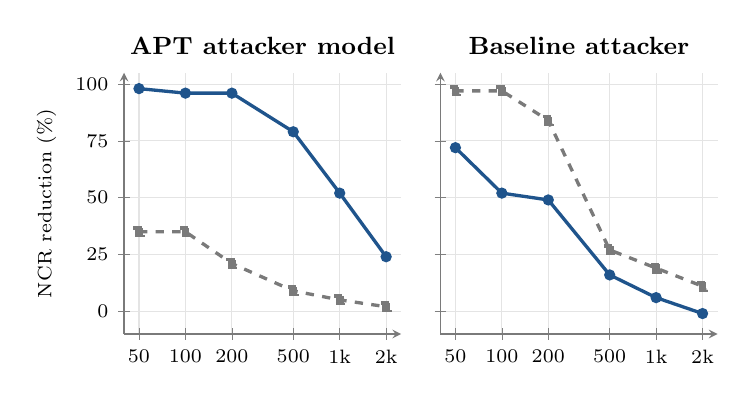
\begin{tikzpicture}
\begin{groupplot}[
  group style={group size=2 by 1, horizontal sep=5mm, y descriptions at=edge left},
  width=5.1cm, height=4.9cm, legend to name=layers,
  xmode=log, xmin=40, xmax=2500,
  xtick={50,100,200,500,1000,2000},
  xticklabels={50,100,200,500,1k,2k},
  ymin=-10, ymax=105, ytick={0,25,50,75,100},
  tick label style={font=\scriptsize},
  label style={font=\scriptsize},
  title style={font=\small\bfseries, yshift=-1mm},
  axis lines=left, axis line style={mid},
  grid=major, grid style={mid!20},
  legend style={font=\scriptsize, draw=none, legend columns=2, /tikz/every even column/.append style={column sep=4mm}},
]
\nextgroupplot[title={APT attacker model}, ylabel={NCR reduction (\%)}]
  \addplot[accent, very thick, mark=*, mark size=1.4pt] coordinates {(50,98)(100,96)(200,96)(500,79)(1000,52)(2000,24)};
  \addplot[mid, very thick, dashed, mark=square*, mark size=1.4pt] coordinates {(50,35)(100,35)(200,21)(500,9)(1000,5)(2000,2)};
\nextgroupplot[title={Baseline attacker}]
  \addplot[accent, very thick, mark=*, mark size=1.4pt] coordinates {(50,72)(100,52)(200,49)(500,16)(1000,6)(2000,-1)};
  \addplot[mid, very thick, dashed, mark=square*, mark size=1.4pt] coordinates {(50,97)(100,97)(200,84)(500,27)(1000,19)(2000,11)};
  \legend{host layer, service layer}
\end{groupplot}
\end{tikzpicture}\\[-0.5mm]
{\scriptsize Deployment interval (s, log scale)}\\[0.5mm]
\ref{layers}
\end{column}
\begin{column}{0.38\textwidth}
\textbf{Why} (measured at 2\,000\,s):
\begin{itemize}
  \item The service layer disrupts only port scans, exploits and brute force
  \item Blocks an attack action: 95\,\% baseline, 15\,\% APT model
  \item Host layer costs the APT model 242 to 324\,s
\end{itemize}
\end{column}
\end{columns}
\end{frame}
\note[itemize]{
\item \textbf{9:45 to 11:15.} Left: in each panel, which line is on top? APT attacker model: host layer, at every interval. Baseline attacker: service layer, at every interval. Each line is the mean over the layer's mechanisms.
\item The host layer keeps at least half of the APT attacker model's NCR off up to 1\,000\,s; the service layer does that for the baseline attacker only up to 200\,s.
\item Why: a deployment disrupts an attacker only if it lands while the attacker is doing what that layer breaks. The baseline attacker scans ports, exploits and brute-forces back to back; the APT attacker model sits mostly in unmapped tactics, which run no attack action.
\item A host-layer deployment costs the APT attacker model 242 to 324\,s: it has no host until its Petri net next reaches Lateral Movement. The baseline attacker loses none, because its procedure re-enumerates a host at once.
\item Say ``likely'': the tactic durations and the order of the tactics most likely explain it; no run separates the two.
\item Likely question: ``Does the host layer just stop it getting in?'' $\to$ backup \textit{Footholds under the host layer}. Answer: largely yes, at short intervals.
}

% ============================================================================
\section{So what}
% Ch6 6.4; Table F.2 (200 s); Appendix E.5.
\begin{frame}{The attacker model can decide which MTD looks best}
\begin{columns}[T]
\begin{column}{0.46\textwidth}
\centering
\small
\textbf{MTDShield}, learned against the baseline attacker\\[2mm]
\begin{tabular}{@{}l r r@{}}
\toprule
NCR reduction, 200\,s & Baseline & APT model \\
\midrule
MTDShield & \textbf{68\,\%} & 28\,\% \\
random deployment & 33\,\% & \textbf{75\,\%} \\
\bottomrule
\end{tabular}
\end{column}
\begin{column}{0.50\textwidth}
\begin{itemize}
  \item Test a learned strategy on an attacker it was not trained on
  \item Report a ranking with its attacker model
  \item Cost depends on the attacker model
\end{itemize}
\end{column}
\end{columns}
\takeaway{One simplified attacker cannot tell you how MTD performs against an APT.}
\end{frame}
\note[itemize]{
\item \textbf{11:15 to 12:45.} The ``so what'' for anyone who evaluates MTD.
\item MTDShield was trained and tested by Tay against the baseline attacker. It deploys service diversity in 70\,\% or more of its decisions against either attacker. Against the APT attacker model, random deployment does almost three times better. Most likely it learned the mechanism that disrupts its training attacker: a test in the training environment is a test on training data.
\item Fair to Tay: it runs as released, outside its training conditions; this bounds MTDShield as released, not retrained.
\item Recommendation 1: test a learned deployment strategy against an attacker model it was not trained on, beside random deployment over the same mechanisms.
\item Recommendation 2: report each ranking with the attacker model behind it; compare across studies only on a shared attacker model.
\item Recommendation 3, cost: to halve NCR, service diversity deploys every 1\,000\,s against the baseline attacker, but every 100\,s against the APT attacker model: ten times the overhead.
\item Optional question to the room: ``If you were choosing an MTD for a real network, which attacker model would you trust?''
}

% ============================================================================
\section{Conclusion}
% Ch6 6.5 (limitations; T1, T4, T5, T10, T11).
\begin{frame}{Limitations}
\begin{itemize}
  \item One simulator, one network size, no deployment cost
  \item Six attack actions: no data theft, no IDS
  \item Declared durations and failure matrix
  \item 38 attack flows
  \item Cause not isolated
\end{itemize}
\end{frame}
\note[itemize]{
\item \textbf{12:45 to 13:45.} State these yourself before anyone asks; examiners mark you for it.
\item One simulator: every claim holds in MTDSim, on its default 50-host network, with deployments that cost nothing.
\item MTDSim's six attack actions cap the model: 7 of 15 tactics unmapped, so no data theft, no impact, and no IDS to evade.
\item Declared values: tactic durations and failure matrix are judgement where threat reports are silent, fixed before any result. Only the 45\,s duration moves NCR much, and the ranking holds from a quarter to four times it.
\item Small corpus: 38 attack flows, 18 attributed to a known group; three attack profiles rest on 5 to 7.
\item Cause not isolated: tactic durations or the order of tactics. MTDSim's disruption rules were written for the baseline attacker; an APT holding a host through Command and Control might survive an IP shuffle. Both attackers meet the same rules, so the comparison is fair.
\item The headline does not say ``MTD fails against APTs'' or ``my attacker is the realistic one''. It says the ranking \emph{can depend} on the attacker model.
\item Likely question: ``How do you know the code does what you say?'' $\to$ backup \textit{Verification}.
}

% ============================================================================
% Ch7 drafting notes; Table 6.1; Section 7.2.
\begin{frame}{In MTDSim, the most effective MTD depends on the attacker model}
\begin{itemize}
  \item \textbf{Built}: an APT attacker model from 38 attack flows, runnable in MTDSim
  \item \textbf{Found}: host layer against it, service layer against the baseline attacker
  \item \textbf{Next}: richer attack actions, an IDS, deployment cost
\end{itemize}
\takeaway{Evaluate MTD against attacker models grounded in documented behaviour.}
\end{frame}
\note[itemize]{
\item \textbf{13:45 to 14:45.} Answer the research question in one sentence, then the two contributions. No new numbers; the audience has 92 against 36\,\%.
\item Contribution 1: the APT attacker model, which any MTDSim study can run in place of the baseline attacker. Two of the eight properties in full and three in part, against at most one in full for three recent models. A proof of concept, built, run and open-sourced; not a claim that it reproduces APT behaviour.
\item Contribution 2: the finding. At every deployment interval, the host layer disrupts the APT attacker model most and the service layer the baseline attacker.
\item Future work: attack actions for actions on objectives, and an IDS; separate the tactic durations from the order of tactics; deployment cost; other networks; MTDShield retrained against the APT attacker model.
\item Then move to the questions slide.
}

% ============================================================================
\begin{frame}[plain,noframenumbering]
\centering
\vfill
{\Huge\color{accent}\textbf{Questions?}}\\[8mm]
{\large How does MTD perform against APT attackers?}\\[2mm]
{\normalsize In MTDSim, it depends on which attacker it is tested against.}\\[10mm]
{\small\color{mid} Marc Labouchardiere \quad\textbullet\quad Supervisor: Dr Jin B. Hong}\\[1mm]
{\small\color{mid} Code and experiments: github.com/marc-la/MTDSim}
\vfill
\end{frame}
\note[itemize]{
\item Leave this up during questions.
\item Q\&A map: weaker attacker $\to$ \textit{Why it compromises less}; footholds $\to$ \textit{Footholds}; durations $\to$ \textit{Tactic durations}; components $\to$ \textit{Ablations}; per profile $\to$ \textit{Each attack profile}; scoring $\to$ \textit{Scoring}; Petri net $\to$ \textit{The Petri net}; MTDShield $\to$ \textit{MTDShield as run}; ASP $\to$ \textit{Disruption and ASP}; earlier numbers $\to$ \textit{Verification}.
}

% ============================================================================
% =========================== BACKUP SLIDES ==================================
% ============================================================================
\appendix
\setbeamertemplate{footline}{\hfill{\scriptsize\color{mid}Backup \insertframenumber}\hspace*{4mm}\vspace{2mm}}

% Ch6 6.1; Appendix G.3, Tables G.5 and G.6; T2.
\begin{frame}{Backup: why the APT attacker model compromises less with no MTD}
\begin{itemize}
  \item Unmapped tactics take 34 to 57\,\% of an attack profile's run, and 15 to 30\,\% of its attack actions fail because their preconditions are missing (e.g.\ exploit before scan port)
  \item Rerun with the baseline attacker's times in place of its tactic durations, same order of tactics: ASP rises from 0.09 to 0.45, against the baseline attacker's 0.66, closing 63\,\% of the gap
  \item The order of its tactics most likely accounts for the rest
  \item The rankings compare each attacker with its own NCR with no MTD, so the lower starting point is unlikely to decide which mechanism ranks first
\end{itemize}
\vfill{\scriptsize Dissertation Section 6.1, Appendix G.3, threat T2. Appendix G analyses were chosen after the results were seen (T9).}
\end{frame}

% Appendix G.4, Table G.7.
\begin{frame}{Backup: footholds under the host layer}
\begin{itemize}
  \item Under the three host-layer mechanisms at 50 to 200\,s, 70 to 89\,\% of the APT attacker model's runs compromise no host, against 3 to 20\,\% of the baseline attacker's
  \item With no MTD: 1\,\% and none
  \item So the host layer disrupts the APT attacker model mostly \emph{before} its first foothold: after a host-layer deployment it has no host until its Petri net next reaches Lateral Movement
  \item From 500\,s the share falls for both attackers, and the host layer still ranks first against the APT attacker model
\end{itemize}
\vfill{\scriptsize Dissertation Appendix G.4 (post hoc, T9); the claim stands on Chapter 5 without it.}
\end{frame}

% Appendix D.1, Tables D.3 and D.4.
\begin{frame}{Backup: are the declared tactic durations driving the result?}
\begin{columns}[T]
\begin{column}{0.48\textwidth}
\small
\begin{tabular}{@{}l r r r@{}}
\toprule
Mean duration (band) & low & declared & high \\
\midrule
4.5\,s (2.25 to 9) & 0.165 & 0.163 & 0.159 \\
35\,s (17.5 to 70) & 0.172 & 0.163 & 0.145 \\
36\,s (18 to 72) & 0.170 & 0.163 & 0.148 \\
45\,s (11.25 to 180) & \textbf{0.267} & 0.163 & \textbf{0.059} \\
\bottomrule
\end{tabular}\\[1mm]
{\scriptsize NCR with no MTD, each value moved alone, 400 runs per cell.}
\end{column}
\begin{column}{0.48\textwidth}
\begin{itemize}
  \item Bands fixed before the run; one value moved at a time
  \item Only the 45\,s (Persistence, Stealth, Command and Control) moves NCR much: Command and Control is the only tactic that finds new hosts
  \item At a quarter and four times the 45\,s, rank 1 still shares no mechanism with the baseline attacker's, and the host layer still ranks above the service layer ($\rho = 0.03$ and $-0.03$)
  \item Untested: interactions between values
\end{itemize}
\end{column}
\end{columns}
\vfill{\scriptsize Dissertation Appendix D.1, threat T4.}
\end{frame}

% Section 5.4, Table 5.4.
\begin{frame}{Backup: what each component of the APT attacker model changes}
\centering
\small
\begin{tabular}{@{}l l r r r@{}}
\toprule
Component removed & MTD & NCR with & without & Cohen's $d$ \\
\midrule
Attack profiles (use the whole attack graph) & no MTD & 0.171 & 0.189 & \textbf{$-0.28$} \\
 & IP shuffle, 200\,s & 0.007 & 0.013 & \textbf{$-0.47$} \\
 & OS diversity, 200\,s & 0.159 & 0.174 & \textbf{$-0.26$} \\
\midrule
Failure matrix & no MTD & 0.171 & 0.167 & $+0.07$ \\
 & IP shuffle, 200\,s & 0.007 & 0.006 & $+0.13$ \\
\midrule
Vulnerability memory & no MTD & 0.171 & 0.169 & $+0.04$ \\
 & service diversity, 200\,s & 0.109 & 0.106 & $+0.07$ \\
\bottomrule
\end{tabular}\\[2mm]
\raggedright
\begin{itemize}
  \item Bold: not negligible ($|d| > 0.2$). The failure matrix changes \emph{where} the attacker goes after a failure (back to Reconnaissance 76 to 83\,\% vs 8 to 10\,\%), not what it achieves
  \item Without the attack profiles, the same three host-layer mechanisms still rank first
\end{itemize}
\end{frame}

% Figure 5.4.
\begin{frame}{Backup: each attack profile against the baseline attacker}
\centering
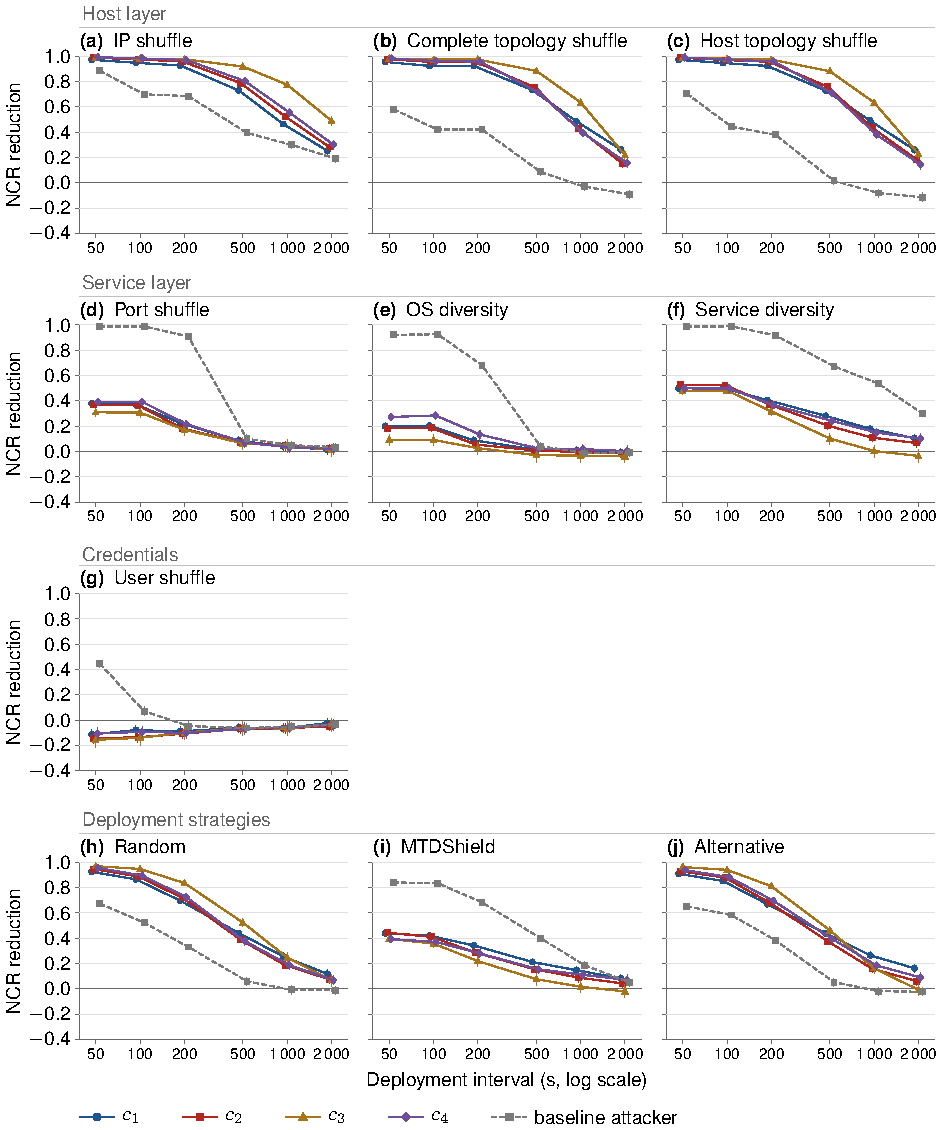
\includegraphics[height=0.80\textheight]{fig_5-3-3b_interval_mechanisms}\\
{\scriptsize At 50 to 200\,s the four attack profiles differ from one another less than the baseline attacker differs from the nearest of them (dissertation Figure 5.4).}
\end{frame}

% Table 6.1, Section 3.3.2, T7.
\begin{frame}{Backup: scoring the eight properties}
\centering
\small
\begin{tabular}{@{}l c c c c c c c c@{}}
\toprule
 & 1 & 2 & 3 & 4 & 5 & 6 & 7 & 8 \\
Attacker model & Pers. & Obj. & Strat. & Adapt. & Detect. & Cost & Learn. & Deploy. \\
\midrule
Baseline attacker (2023) & \yes & \no & part & part & \no & \no & \no & \no \\
Masud et al.\ (2025) & part & \no & \no & \no & \no & \no & \no & \no \\
Kim et al.\ (2026) & part & \no & \no & \no & part & \no & \no & \no \\
\textbf{APT attacker model} & \yes & part & \yes & part & part & \no & \no & \no \\
\bottomrule
\end{tabular}\\[2mm]
\raggedright
\begin{itemize}
  \item Each property split into predicates; \yes{} = every predicate true of the model's own behaviour; part = a behaviour predicate true, but set by a fixed rule or assumed
  \item One scorer, checked by blind scoring with language models (dissertation Appendix B)
  \item Adaptivity is in part because the failure matrix is a fixed rule of mine; detection avoidance in part because MTDSim has no IDS
\end{itemize}
\end{frame}

% Section 4.3, Equations 4.2 and 4.4, Figure 4.4.
\begin{frame}{Backup: the Petri net}
\begin{columns}[T]
\begin{column}{0.52\textwidth}
\centering
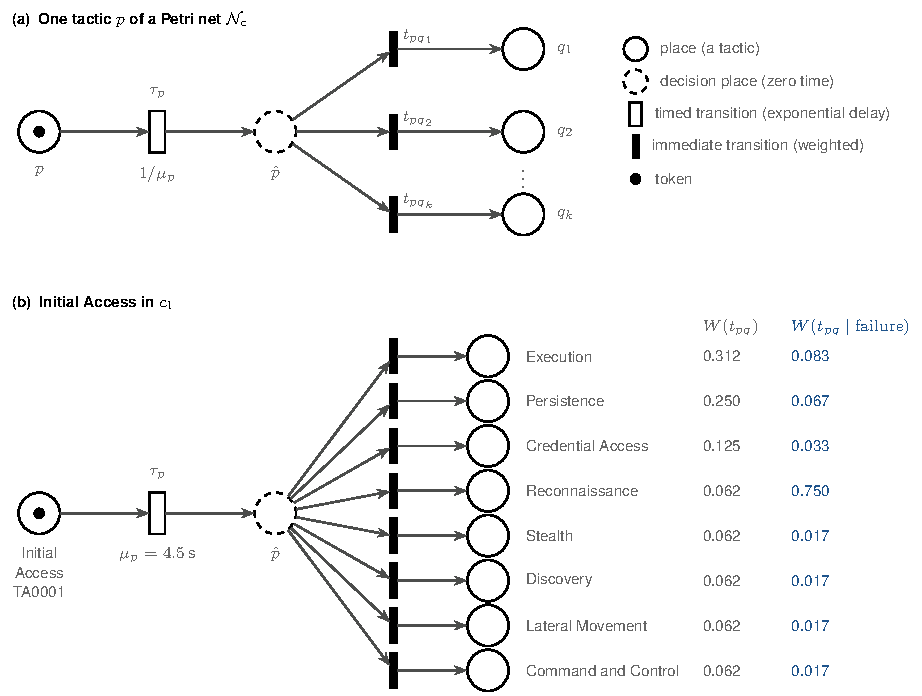
\includegraphics[width=\linewidth]{fig_4-3a_gspn_gadget}
\end{column}
\begin{column}{0.45\textwidth}
\small
Generalised stochastic Petri net \src{Ajmone Marsan 1995}, extended with the failure matrix $F$:
\[(P, T, I, O, W, M_0, F)\]
Base weight of the move from tactic $p$ to $q$:
\[W(t_{pq}) = \frac{n(p,q)}{\sum_{q'} n(p,q')}\]
with $n(p,q)$ the attack flows that draw $p \to q$. After a failed attack action:
\[W(t_{pq}\mid\text{failure}) = \frac{W(t_{pq})\,F(p,q)}{\sum_{q'} W(t_{pq'})\,F(p,q')}\]
One token, starting on Reconnaissance.
\end{column}
\end{columns}
\end{frame}

% Table 4.2, Figure 4.6.
\begin{frame}{Backup: tactic durations and the tactic-to-action mapping}
\begin{columns}[T]
\begin{column}{0.50\textwidth}
\small
\begin{tabular}{@{}>{\raggedright\arraybackslash}p{0.72\linewidth} r@{}}
\toprule
Tactics & Mean (s) \\
\midrule
Initial Access, Privilege Escalation, Credential Access, Lateral Movement {\scriptsize(MTDSim's exploit)} & 4.5 \\
Reconnaissance, Discovery {\scriptsize(MTDSim's three scans)} & 35 \\
Persistence, Stealth, Command and Control & 45 \\
Collection, Exfiltration, Impact & 36 \\
Execution, Defense Impairment & 22.5 \\
Resource Development & 0 \\
\bottomrule
\end{tabular}\\[1mm]
{\scriptsize Last four rows: judgement, kept on the baseline attacker's time scale and under the 200\,s default interval.}
\end{column}
\begin{column}{0.46\textwidth}
\centering
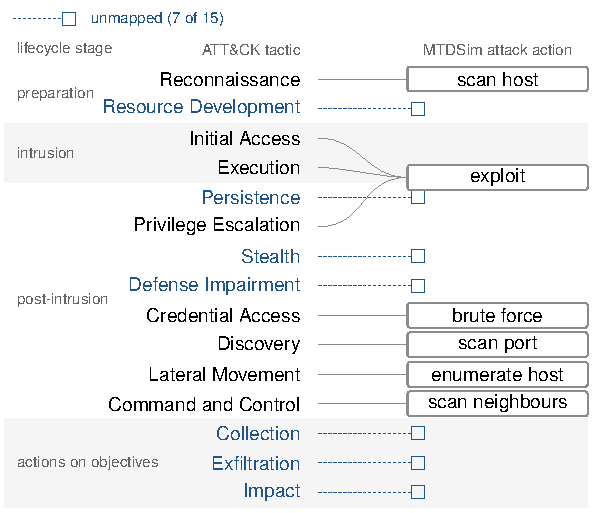
\includegraphics[width=\linewidth]{fig_4-4a_controller_mapping}
\end{column}
\end{columns}
\end{frame}

% Appendix E.4 and E.5.
\begin{frame}{Backup: MTDShield as run}
\begin{itemize}
  \item Run as released by Tay (2024); correcting the release would make it my agent, not Tay's
  \item Trained at one deployment interval, against the baseline attacker, on 100-host networks
  \item Known limits of the release: published scores produced with exploration at one; four evaluation inputs read as zero; ``do nothing'' never a learning target
  \item Its detection input reads an unmapped tactic as ``nothing detected''
  \item So the result bounds MTDShield \emph{as released}, not MTDShield retrained against the APT attacker model
\end{itemize}
\vfill{\scriptsize Dissertation Appendix E, threat T12.}
\end{frame}

% Figure 5.2; Appendix F.1, Table F.3.
\begin{frame}{Backup: disruption per MTD deployment, and ASP}
\begin{columns}[T]
\begin{column}{0.58\textwidth}
\centering
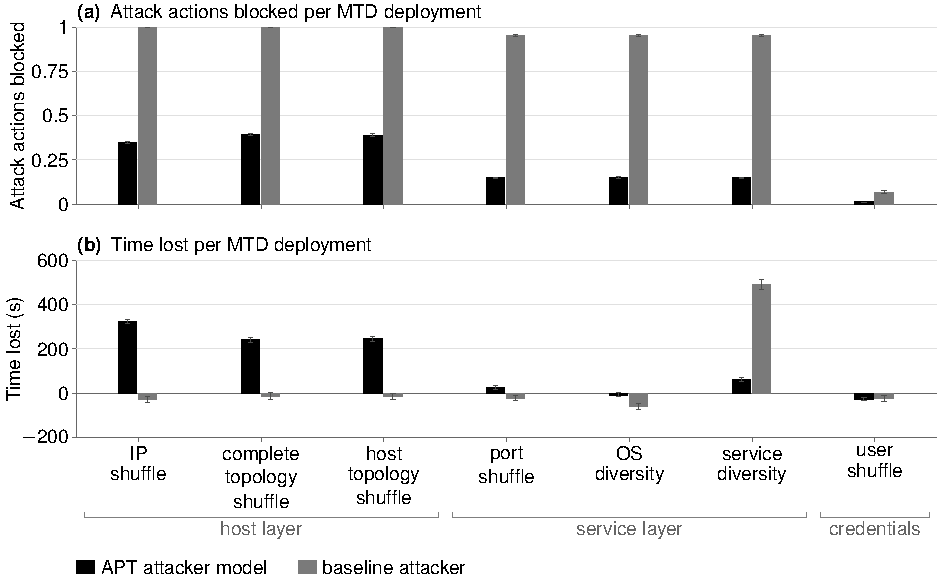
\includegraphics[width=\linewidth]{fig_5-2-2a_disruption_response}
\end{column}
\begin{column}{0.39\textwidth}
\begin{itemize}
  \item Measured at 2\,000\,s, because the next deployment caps time lost at the interval
  \item The baseline attacker's time lost is at or below zero after the first deployment: sent back to scan host, it gets a second attempt at its first host, as MTDSim intends
  \item On ASP reduction the layer order also holds against each attacker (Table F.3)
\end{itemize}
\end{column}
\end{columns}
\end{frame}

% T3.
\begin{frame}{Backup: verification, and why no comparison with earlier MTDSim numbers}
\begin{itemize}
  \item An event tracer replays any run step by step, across Petri net, attacker and MTD
  \item MTDSim's code audited against what its papers describe; unit tests of the Petri net and the simulator
  \item Fixed seeds reproduce every run exactly
  \item Defects found in MTDSim were repaired before the evaluation, so results are not compared numerically with Zhang (2023) or Tay (2024)
\end{itemize}
\vfill{\scriptsize Dissertation threat T3.}
\end{frame}

\begin{frame}{References}
\scriptsize
\begin{itemize}
  \item[] A.~Alshamrani et al., ``A survey on advanced persistent threats,'' \emph{IEEE Commun.\ Surveys Tuts.}, 21(2), 2019.
  \item[] M.~Ajmone Marsan et al., \emph{Modelling with Generalized Stochastic Petri Nets}, Wiley, 1995.
  \item[] A.~Brown, T.-W.~Lee and J.~B.~Hong, ``Evaluating moving target defenses against realistic attack scenarios,'' EnCyCriS, 2023.
  \item[] Center for Threat-Informed Defense, ``Attack Flow,'' MITRE, v3.2.0, 2025.
  \item[] J.-H.~Cho et al., ``Toward proactive, adaptive defense: A survey on moving target defense,'' \emph{IEEE Commun.\ Surveys Tuts.}, 22(1), 2020.
  \item[] CISA et al., ``PRC state-sponsored actors compromise and maintain persistent access to U.S.\ critical infrastructure,'' Advisory AA24-038A, 2024.
  \item[] {\L}.~Jalowski et al., ``Rethinking the security assurances of MTD: A gap analysis for network defense,'' \emph{Future Internet}, 18(2), 2026.
  \item[] M.~Kim et al., ``MTD in depth: Multi-phased moving target defense techniques against cyber-attacks based on cyber kill chain,'' \emph{FGCS}, 181, 2026.
  \item[] M.~T.~Masud et al., ``Vulnerability defence using hybrid moving target defence in Internet of Things systems,'' \emph{Computers \& Security}, 153, 2025.
  \item[] Joint Task Force, ``Managing information security risk,'' NIST SP 800-39, 2011.
  \item[] C.~Tantithamthavorn et al., ``An empirical comparison of model validation techniques for defect prediction models,'' \emph{IEEE TSE}, 43(1), 2017.
  \item[] J.~K.~Tay, ``Using artificial intelligence to automate the deployment of moving target defence operations,'' UWA research report, 2024.
  \item[] W.~Zhang, ``Evaluating multiple moving target defence in the time domain,'' Master's thesis, UWA, 2023.
\end{itemize}
\end{frame}

\end{document}
"  (twice)
% Slides carry prompts only; what to say is in each frame's \note.
% Every number on a slide is taken from the dissertation; the table or
% figure it comes from is named in the frame's comment.
\documentclass[aspectratio=169,11pt]{beamer}

\usepackage[T1]{fontenc}
\usepackage[scaled=0.92]{helvet}   % the figures' face
\usepackage{booktabs}
\usepackage{array}
\usepackage{tabularx}
\usepackage{pifont}
\usepackage{pgfplots}
\pgfplotsset{compat=1.17}
\usepgfplotslibrary{groupplots}
\usepackage{appendixnumberbeamer}   % "n / 12" counts the main slides only
\graphicspath{{../figures/}}

\ifdefined\withnotes
  \setbeameroption{show notes}
\fi

% --- look: plain, legible, one accent ---------------------------------------
\definecolor{accent}{RGB}{31,84,140}
\definecolor{mid}{RGB}{122,122,122}
\setbeamertemplate{navigation symbols}{}
\setbeamercolor{frametitle}{fg=accent}
\setbeamerfont{frametitle}{size=\large,series=\bfseries}
\setbeamercolor{structure}{fg=accent}
\setbeamertemplate{itemize items}{\color{accent}\textbullet}
\setbeamertemplate{itemize subitem}{\color{mid}--}
\setbeamersize{text margin left=8mm,text margin right=8mm}

% --- footer: the talk's timeline (sections, one dot per slide) + n / 12 -----
\useoutertheme[subsection=false]{miniframes}
\setbeamertemplate{headline}{}
\setbeamertemplate{mini frames}[default]
\setbeamercolor{section in head/foot}{fg=accent}
\setbeamercolor{mini frame}{fg=accent}
\setbeamerfont{section in head/foot}{size=\scriptsize}
\setbeamertemplate{footline}{%
  \begin{beamercolorbox}[wd=\paperwidth,ht=4mm,dp=3.6mm]{section in head/foot}%
    \hspace*{2mm}\insertnavigation{0.82\paperwidth}\hfill
    {\scriptsize\color{mid}\insertframenumber\,/\,\inserttotalframenumber}\hspace*{4mm}%
  \end{beamercolorbox}}

\newcommand{\src}[1]{{\scriptsize\color{mid}[#1]}}
\newcommand{\yes}{\ding{51}}
\newcommand{\no}{{\color{mid}\ding{55}}}
\newcommand{\takeaway}[1]{\vfill{\color{accent}\rule{\linewidth}{0.4pt}}\\[1mm]#1\vspace{1mm}}

\title{Evaluating moving target defence against advanced persistent threat attackers modelled on documented intrusion campaigns}
\author{Marc Labouchardiere\\[1mm]{\small Supervisor: Dr Jin B. Hong}}
\institute{\small Honours seminar, The University of Western Australia}
\date{\small 2026}

\begin{document}

% ============================================================================
\begin{frame}[plain,noframenumbering]
  \titlepage
\end{frame}
\note[itemize]{
\item \textbf{0:00 to 0:15.} Name, supervisor.
\item One line: ``I test whether MTD's measured effectiveness survives a change of attacker.''
\item The footer is the talk's timeline: six parts, one dot per slide.
}

% ============================================================================
\section{Motivation}
% Ch1; ch3 3.1.1 and 3.1.3; Figure 3.2.
\begin{frame}{MTD is proposed against APT attackers, but rarely tested against one}
\begin{columns}[T]
\begin{column}{0.44\textwidth}
\begin{itemize}
  \item \textbf{Advanced persistent threat (APT)}: one target, months to years
  \item Volt Typhoon: five years inside US infrastructure \src{CISA 2024}
  \item \textbf{Moving target defence (MTD)}: keep the network moving
  \item Tested against simple, scripted attackers
\end{itemize}
\end{column}
\begin{column}{0.53\textwidth}
  \centering
  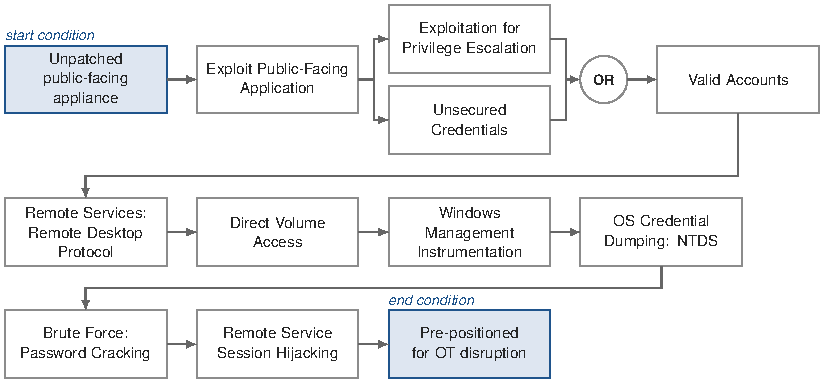
\includegraphics[width=\linewidth]{fig_3-1-3a_attack_flow_volt_typhoon}\\[1mm]
  {\scriptsize Volt Typhoon's intrusion as an \textbf{attack flow}}
\end{column}
\end{columns}
\takeaway{\textbf{Research question:} How does MTD perform against APT attackers?}
\end{frame}
\note[itemize]{
\item \textbf{0:15 to 1:30.} APT: a well-resourced attacker, often state-sponsored, pursuing one objective against one target over months or years (Alshamrani 2019). Espionage intrusions go undetected for a median of 122 days (Mandiant 2026).
\item Volt Typhoon held footholds in US critical infrastructure for at least five years, signing in with stolen valid accounts. Its reconnaissance stayed valid because the networks never changed.
\item MTD: change addresses, topology, software and credentials on a schedule, so what the attacker learned goes out of date even if it is never detected (Cho 2020).
\item Point at the attack flow: ``This is what a threat report gives us: the steps, in order, drawn by an analyst. It is the raw material of my attacker.''
\item The gap: MTD is proposed against APTs, but tested in simulation against attackers far simpler than an APT (Jalowski 2026). Read the research question aloud.
\item Transition: ``To test that, I need an MTD simulator and an attacker.''
}

% ============================================================================
\section{Previous work}
% Ch2: Figure 2.2, Table 2.1, Section 2.2.3.
\begin{frame}{MTDSim: seven MTD mechanisms, one scripted attacker}
\begin{columns}[T]
\begin{column}{0.44\textwidth}
\begin{itemize}
  \item \textbf{MTDSim} \src{Brown 2023; Zhang 2023; Tay 2024}
  \item \textbf{Host layer}: where hosts are
  \item \textbf{Service layer}: what runs on them
  \item \textbf{Baseline attacker}: six \textbf{attack actions}, fixed order
\end{itemize}
\end{column}
\begin{column}{0.53\textwidth}
  \centering
  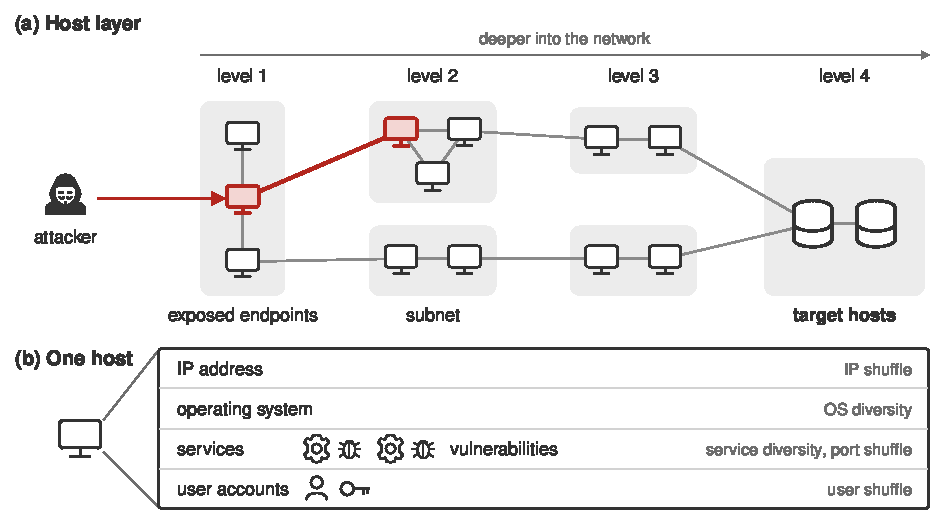
\includegraphics[width=\linewidth]{fig_2-2-1a_network_model}
\end{column}
\end{columns}
\end{frame}
\note[itemize]{
\item \textbf{1:30 to 2:30.} The work I inherit: Brown built MTDSim at UWA, Zhang added simulated time, Tay added MTDShield, a reinforcement-learning agent that picks which mechanism to deploy.
\item Panel (a): 50 hosts in four levels; the attacker enters at an exposed endpoint and works towards the target hosts.
\item Panel (b): each part of a host has a mechanism that moves it. Seven MTD mechanisms, one deployed every deployment interval (200\,s by default).
\item \textbf{The two layers the results hinge on}: host layer = IP shuffle and two topology shuffles; service layer = port shuffle, OS diversity, service diversity. Plus user shuffle on credentials.
\item Baseline attacker: scan host, enumerate host, scan port, exploit, brute force, scan neighbours; the same order every run.
\item Transition: ``Is a fixed procedure a fair stand-in for an APT?''
}

% ============================================================================
% Ch3: Tables 3.2 and 3.3.
\begin{frame}{Recent MTD attacker models lack most APT properties}
\centering
\small
\begin{tabular}{@{}l l c c c@{}}
\toprule
 & Property & Baseline attacker & Masud et al. & Kim et al. \\
 & & {\scriptsize 2023} & {\scriptsize 2025} & {\scriptsize 2026} \\
\midrule
1 & Campaign persistence & \yes & part & part \\
2 & Objective-specific behaviour & \no & \no & \no \\
3 & Choice of attack strategy & part & \no & \no \\
4 & Adaptivity to MTD disruption & part & \no & \no \\
5 & Detection avoidance & \no & \no & part \\
6 & Cost--benefit reasoning & \no & \no & \no \\
7 & Learning from past deployments & \no & \no & \no \\
8 & Deployment-strategy awareness & \no & \no & \no \\
\bottomrule
\end{tabular}\\[1mm]
{\scriptsize 1, 2, 4, 5: the APT definition \src{Alshamrani 2019; NIST 2011}. 3, 6, 7, 8: two MTD surveys \src{Cho 2020; Jalowski 2026}.}
\takeaway{\textbf{Gap}: how MTD performs against APT attackers is unmeasured.}
\end{frame}
\note[itemize]{
\item \textbf{2:30 to 3:30.} Eight properties: four from what an APT is, four that two MTD surveys say attacker models lack. Jalowski et al. call the attacker model ``the most glaring flaw in the MTD literature''.
\item I scored the baseline attacker and the two most recent MTD evaluations that describe their attacker in Kill Chain or ATT\&CK terms, the ones I expected to do best.
\item Read the result: at most one property in full, campaign persistence, only for the baseline attacker. None has objective-specific behaviour.
\item I targeted three: objective-specific behaviour, choice of attack strategy, adaptivity.
\item Likely question: ``How did you score them?'' $\to$ backup \textit{Scoring the eight properties}.
}

% ============================================================================
\section{Method}
% Ch4: Figure 4.1, Section 4.1, Table 4.1.
\begin{frame}{Build an APT attacker model from threat reports; run it in MTDSim}
\begin{columns}[T]
\begin{column}{0.60\textwidth}
  \centering
  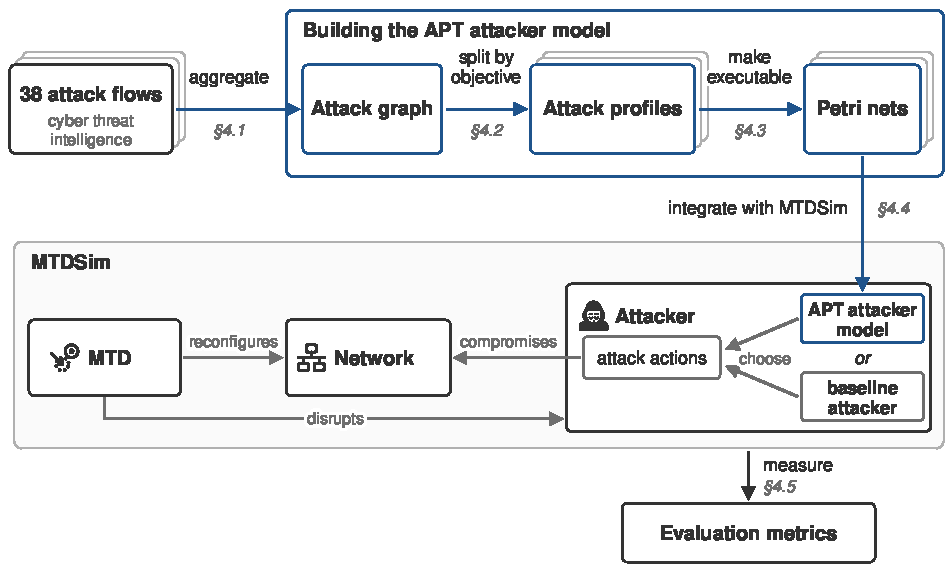
\includegraphics[width=\linewidth]{fig_4-0a_method_overview}
\end{column}
\begin{column}{0.37\textwidth}
\begin{itemize}
  \item \textbf{SQ1}: 38 attack flows $\to$ four \textbf{attack profiles} by objective
  \item \textbf{SQ2}: each runs as a Petri net
  \item \textbf{SQ3}: two attackers, same MTD
\end{itemize}
\vspace{2mm}
{\small
\begin{tabular}{@{}l l@{}}
c1 & stole data \\
c2 & impeded systems \\
c3 & both \\
c4 & neither \\
\end{tabular}}
\end{column}
\end{columns}
\end{frame}
\note[itemize]{
\item \textbf{3:30 to 4:45.} Three sub-questions, one pipeline: point left to right along the top row.
\item The 38 attack flows are analysts' hand-drawn graphs of reported intrusions, published by MITRE's Center for Threat-Informed Defense; the Volt Typhoon picture is one of the kind. Hand-drawn matters: automated extraction from report text is unreliable (best systems 80\,\% precision at 66\,\% recall on identifying techniques alone).
\item Aggregated into an attack graph over the 15 ATT\&CK tactics (what the attacker is trying to do: Initial Access, Lateral Movement, Exfiltration, \ldots). Tactics, not techniques: 88\,\% of technique-to-technique edges come from a single attack flow.
\item Split by two yes/no questions per attack flow: did it steal data, did it impede systems. c1 has 19 attack flows, c2 7, c3 7 (mostly ransomware), c4 5.
\item Transition: ``A graph does not run. Here is how it runs.''
}

% ============================================================================
% Ch4: Figure 4.5; Sections 4.3, 4.4.1 to 4.4.3; Figure 4.4(b).
\begin{frame}{A Petri net picks the next tactic; MTDSim carries it out}
\begin{columns}[T]
\begin{column}{0.62\textwidth}
  \centering
  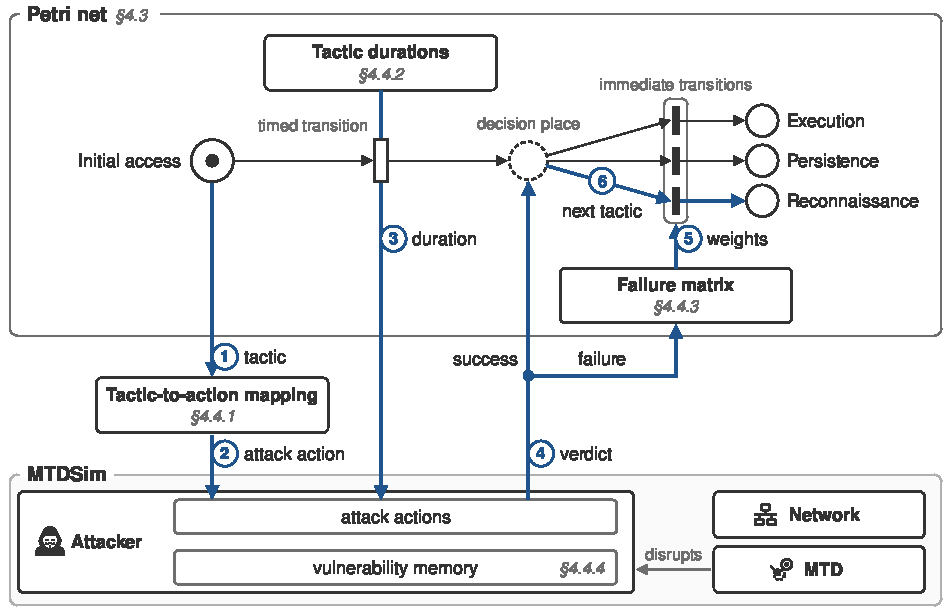
\includegraphics[width=\linewidth]{fig_4-4c_runtime_loop}
\end{column}
\begin{column}{0.35\textwidth}
\begin{itemize}
  \item Next tactic: drawn from the attack flows
  \item 7 of 15 tactics \textbf{unmapped}
  \item Timing and failures: declared
\end{itemize}
\end{column}
\end{columns}
\end{frame}
\note[itemize]{
\item \textbf{4:45 to 6:15.} Walk the loop once with your finger, steps 1 to 6: the token's tactic leaves the Petri net; the tactic-to-action mapping turns it into an attack action; it runs for the tactic duration; MTDSim returns success or failure; after a failure the failure matrix reweights; the token moves on.
\item Petri net: a generalised stochastic Petri net, the convention in MTD evaluation. Next tactic drawn in proportion to how many attack flows took that step, so runs differ.
\item Tactic-to-action mapping: 8 of 15 tactics run one of MTDSim's six attack actions. The other 7 (e.g.\ Exfiltration, Stealth) are unmapped and only take time. The ceiling: MTDSim's attack actions only find and compromise hosts, so the model steals no data. Say this plainly.
\item Threat reports record no timing and no failures. Tactic durations (up to 45\,s on average) and the failure matrix are declared before any result, then varied. Example: a failed Initial Access returns to Reconnaissance with weight 0.75, up from 0.06.
\item Likely questions: ``Why these durations?'' $\to$ backup \textit{Tactic durations}; ``Formal definition?'' $\to$ backup \textit{The Petri net}.
}

% ============================================================================
% Ch5: Table 5.1, Section 4.5.
\begin{frame}{Experiment: both attackers on the same 1\,000 networks}
\begin{columns}[T]
\begin{column}{0.52\textwidth}
\small
\begin{tabularx}{\linewidth}{@{}>{\bfseries}l >{\raggedright\arraybackslash}X@{}}
\toprule
Attacker & baseline; APT model, c1 to c4 \\
MTD & none; 7 mechanisms; 3 deployment strategies \\
Interval & 50 to 2\,000\,s \\
Seeds & 1\,000 per configuration \\
\bottomrule
\end{tabularx}
\end{column}
\begin{column}{0.45\textwidth}
\textbf{NCR}: share of hosts compromised\\[3mm]
\textbf{NCR reduction}\\[1mm]
$\displaystyle = 1 - \frac{\text{NCR under MTD}}{\text{NCR with no MTD}}$
\end{column}
\end{columns}
\end{frame}
\note[itemize]{
\item \textbf{6:15 to 7:00.} Keep this quick.
\item The design choice that matters: every configuration runs on the same 1\,000 seeds, so both attackers face the same 1\,000 networks. Differences come from the attacker, not the network. 1\,000 runs follows the recommendation for randomised algorithms (Arcuri and Briand).
\item MTD: none; each of the seven mechanisms alone; random and alternative rotation; MTDShield as released. Intervals 50, 100, 200, 500, 1\,000, 2\,000\,s.
\item Targeted scenario: a run ends at the first target host compromised, or at 15\,000\,s.
\item NCR, network compromise ratio (Zhang 2023). NCR reduction compares each attacker with its own runs with no MTD: 0 = no effect, 1 = nothing compromised.
\item MTD settings ranked by the Scott--Knott effect-size test; the two rankings compared with Spearman's $\rho$.
}

% ============================================================================
\section{Results}
% Ch5: Table 5.2, Figure 5.1(b), Section 5.2; Ch6 6.1.
\begin{frame}{No MTD: the APT attacker model acts more like an APT, but compromises less}
\small
\begin{tabularx}{\textwidth}{@{}>{\raggedright\arraybackslash}X >{\centering\arraybackslash}p{3.0cm} >{\centering\arraybackslash}p{2.4cm}@{}}
\toprule
 & APT attacker model & Baseline attacker \\
\midrule
Distinct openings (first 8 steps) & 179 to 947 & 3 \\
Attack actions per minute & 0.68 to 1.23 & 1.71 \\
Not flagged by a port-scan rule & 89 to 98\,\% & 82\,\% \\
\midrule
Runs reaching a target host (ASP) & 0.04 to 0.14 & 0.66 \\
Share of hosts compromised (NCR) & 0.15 to 0.21 & 0.50 \\
\bottomrule
\end{tabularx}
\normalsize
\takeaway{Same cause for both halves: its tactic durations and the order of its tactics.}
\end{frame}
\note[itemize]{
\item \textbf{7:00 to 8:15.} First, no MTD at all: does the model behave differently?
\item Row 1, choice of attack strategy: the baseline attacker's 1\,000 runs start the same way; the attack profiles' runs part ways by the second to fourth step. Ranges are over c1 to c4.
\item Rows 2 and 3, detection avoidance by proxy: it acts less often, and Snort's default port-scan rule (5 targets in 60\,s) would flag fewer of its attack actions. MTDSim has no IDS; say so.
\item Objective-specific behaviour (not on the slide): Exfiltration steps only in c1 and c3, Impact mostly in c2 and c3.
\item Bottom rows: it reaches a target in far fewer runs. Pre-empt the objection: ``Yes, with no MTD it is the weaker attacker. ASP and NCR alone would rate it weaker for exactly what makes it APT-like. With the baseline attacker's times it closes about two thirds of the gap.''
\item Transition: ``Two different attackers, the same networks. Now switch MTD on.''
\item Likely question: ``Isn't it just weaker?'' $\to$ backup \textit{Why it compromises less}.
}

% ============================================================================
% Ch5: Table 5.3 (200 s), Table F.4, Section 5.3.2.
\begin{frame}{Headline: the most effective MTD mechanism differs between the attackers}
\begin{columns}[T]
\begin{column}{0.56\textwidth}
\small
\begin{tabular}{@{}l >{\centering\arraybackslash}p{2.1cm} >{\centering\arraybackslash}p{2.1cm}@{}}
\toprule
NCR reduction at 200\,s & APT attacker model & Baseline attacker \\
\midrule
\multicolumn{3}{@{}l}{\textit{host layer}} \\
\quad IP shuffle & \textbf{96\,\% (1)} & 68\,\% (2) \\
\quad complete topology & \textbf{95\,\% (1)} & 42\,\% (3) \\
\quad host topology & \textbf{95\,\% (1)} & 38\,\% (3) \\
\multicolumn{3}{@{}l}{\textit{service layer}} \\
\quad service diversity & 36\,\% (4) & \textbf{92\,\% (1)} \\
\quad port shuffle & 20\,\% (6) & \textbf{91\,\% (1)} \\
\quad OS diversity & 7\,\% (7) & 68\,\% (2) \\
\multicolumn{3}{@{}l}{\textit{credentials}} \\
\quad user shuffle & $-10$\,\% (8) & $-5$\,\% (5) \\
\bottomrule
\end{tabular}\\[1mm]
{\scriptsize (rank) among all ten MTD settings}
\end{column}
\begin{column}{0.40\textwidth}
\begin{itemize}
  \item Rank 1 shares no mechanism
  \item Service diversity: 92 against 36\,\%
  \item Spearman's $\rho = 0.01$
\end{itemize}
\end{column}
\end{columns}
\end{frame}
\note[itemize]{
\item \textbf{8:15 to 9:45.} \textbf{This is the result. Slow down.}
\item Read the bold cells: against the APT attacker model, the host layer ranks first; against the baseline attacker, the service layer. Rank 1 shares no mechanism.
\item The one number: service diversity removes 92\,\% of the baseline attacker's NCR and 36\,\% of the APT attacker model's, on the same networks, with the same deployments.
\item $\rho = 0.01$: the two rankings are uncorrelated. Say ``do not agree'', not ``reversed''.
\item APT attacker model averaged over c1 to c4.
\item Only if asked: user shuffle is negative against the APT attacker model because it redraws accounts but leaves valid the ones the attacker holds, so each deployment is a fresh chance to log in.
\item Transition: ``Is that just the default interval?''
}

% ============================================================================
% Ch5: Figure 5.3 panels (a) and (b), redrawn per attacker from Table F.2; Figure 5.2 / Table F.1; Ch6 6.2.
\begin{frame}{The difference holds at every deployment interval}
\begin{columns}[T]
\begin{column}{0.58\textwidth}
\centering
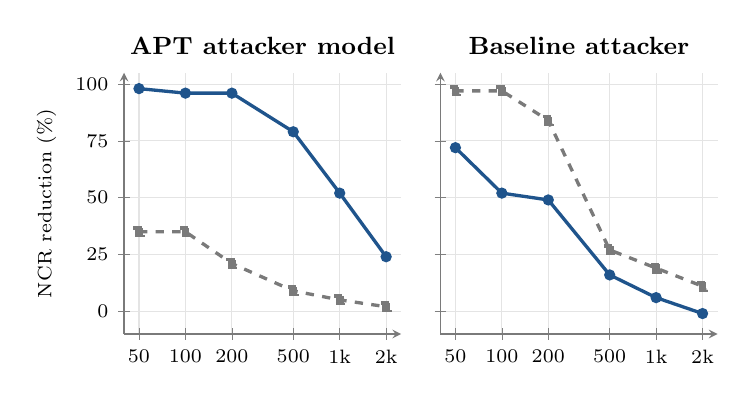
\begin{tikzpicture}
\begin{groupplot}[
  group style={group size=2 by 1, horizontal sep=5mm, y descriptions at=edge left},
  width=5.1cm, height=4.9cm, legend to name=layers,
  xmode=log, xmin=40, xmax=2500,
  xtick={50,100,200,500,1000,2000},
  xticklabels={50,100,200,500,1k,2k},
  ymin=-10, ymax=105, ytick={0,25,50,75,100},
  tick label style={font=\scriptsize},
  label style={font=\scriptsize},
  title style={font=\small\bfseries, yshift=-1mm},
  axis lines=left, axis line style={mid},
  grid=major, grid style={mid!20},
  legend style={font=\scriptsize, draw=none, legend columns=2, /tikz/every even column/.append style={column sep=4mm}},
]
\nextgroupplot[title={APT attacker model}, ylabel={NCR reduction (\%)}]
  \addplot[accent, very thick, mark=*, mark size=1.4pt] coordinates {(50,98)(100,96)(200,96)(500,79)(1000,52)(2000,24)};
  \addplot[mid, very thick, dashed, mark=square*, mark size=1.4pt] coordinates {(50,35)(100,35)(200,21)(500,9)(1000,5)(2000,2)};
\nextgroupplot[title={Baseline attacker}]
  \addplot[accent, very thick, mark=*, mark size=1.4pt] coordinates {(50,72)(100,52)(200,49)(500,16)(1000,6)(2000,-1)};
  \addplot[mid, very thick, dashed, mark=square*, mark size=1.4pt] coordinates {(50,97)(100,97)(200,84)(500,27)(1000,19)(2000,11)};
  \legend{host layer, service layer}
\end{groupplot}
\end{tikzpicture}\\[-0.5mm]
{\scriptsize Deployment interval (s, log scale)}\\[0.5mm]
\ref{layers}
\end{column}
\begin{column}{0.38\textwidth}
\textbf{Why} (measured at 2\,000\,s):
\begin{itemize}
  \item The service layer disrupts only port scans, exploits and brute force
  \item Blocks an attack action: 95\,\% baseline, 15\,\% APT model
  \item Host layer costs the APT model 242 to 324\,s
\end{itemize}
\end{column}
\end{columns}
\end{frame}
\note[itemize]{
\item \textbf{9:45 to 11:15.} Left: in each panel, which line is on top? APT attacker model: host layer, at every interval. Baseline attacker: service layer, at every interval. Each line is the mean over the layer's mechanisms.
\item The host layer keeps at least half of the APT attacker model's NCR off up to 1\,000\,s; the service layer does that for the baseline attacker only up to 200\,s.
\item Why: a deployment disrupts an attacker only if it lands while the attacker is doing what that layer breaks. The baseline attacker scans ports, exploits and brute-forces back to back; the APT attacker model sits mostly in unmapped tactics, which run no attack action.
\item A host-layer deployment costs the APT attacker model 242 to 324\,s: it has no host until its Petri net next reaches Lateral Movement. The baseline attacker loses none, because its procedure re-enumerates a host at once.
\item Say ``likely'': the tactic durations and the order of the tactics most likely explain it; no run separates the two.
\item Likely question: ``Does the host layer just stop it getting in?'' $\to$ backup \textit{Footholds under the host layer}. Answer: largely yes, at short intervals.
}

% ============================================================================
\section{So what}
% Ch6 6.4; Table F.2 (200 s); Appendix E.5.
\begin{frame}{The attacker model can decide which MTD looks best}
\begin{columns}[T]
\begin{column}{0.46\textwidth}
\centering
\small
\textbf{MTDShield}, learned against the baseline attacker\\[2mm]
\begin{tabular}{@{}l r r@{}}
\toprule
NCR reduction, 200\,s & Baseline & APT model \\
\midrule
MTDShield & \textbf{68\,\%} & 28\,\% \\
random deployment & 33\,\% & \textbf{75\,\%} \\
\bottomrule
\end{tabular}
\end{column}
\begin{column}{0.50\textwidth}
\begin{itemize}
  \item Test a learned strategy on an attacker it was not trained on
  \item Report a ranking with its attacker model
  \item Cost depends on the attacker model
\end{itemize}
\end{column}
\end{columns}
\takeaway{One simplified attacker cannot tell you how MTD performs against an APT.}
\end{frame}
\note[itemize]{
\item \textbf{11:15 to 12:45.} The ``so what'' for anyone who evaluates MTD.
\item MTDShield was trained and tested by Tay against the baseline attacker. It deploys service diversity in 70\,\% or more of its decisions against either attacker. Against the APT attacker model, random deployment does almost three times better. Most likely it learned the mechanism that disrupts its training attacker: a test in the training environment is a test on training data.
\item Fair to Tay: it runs as released, outside its training conditions; this bounds MTDShield as released, not retrained.
\item Recommendation 1: test a learned deployment strategy against an attacker model it was not trained on, beside random deployment over the same mechanisms.
\item Recommendation 2: report each ranking with the attacker model behind it; compare across studies only on a shared attacker model.
\item Recommendation 3, cost: to halve NCR, service diversity deploys every 1\,000\,s against the baseline attacker, but every 100\,s against the APT attacker model: ten times the overhead.
\item Optional question to the room: ``If you were choosing an MTD for a real network, which attacker model would you trust?''
}

% ============================================================================
\section{Conclusion}
% Ch6 6.5 (limitations; T1, T4, T5, T10, T11).
\begin{frame}{Limitations}
\begin{itemize}
  \item One simulator, one network size, no deployment cost
  \item Six attack actions: no data theft, no IDS
  \item Declared durations and failure matrix
  \item 38 attack flows
  \item Cause not isolated
\end{itemize}
\end{frame}
\note[itemize]{
\item \textbf{12:45 to 13:45.} State these yourself before anyone asks; examiners mark you for it.
\item One simulator: every claim holds in MTDSim, on its default 50-host network, with deployments that cost nothing.
\item MTDSim's six attack actions cap the model: 7 of 15 tactics unmapped, so no data theft, no impact, and no IDS to evade.
\item Declared values: tactic durations and failure matrix are judgement where threat reports are silent, fixed before any result. Only the 45\,s duration moves NCR much, and the ranking holds from a quarter to four times it.
\item Small corpus: 38 attack flows, 18 attributed to a known group; three attack profiles rest on 5 to 7.
\item Cause not isolated: tactic durations or the order of tactics. MTDSim's disruption rules were written for the baseline attacker; an APT holding a host through Command and Control might survive an IP shuffle. Both attackers meet the same rules, so the comparison is fair.
\item The headline does not say ``MTD fails against APTs'' or ``my attacker is the realistic one''. It says the ranking \emph{can depend} on the attacker model.
\item Likely question: ``How do you know the code does what you say?'' $\to$ backup \textit{Verification}.
}

% ============================================================================
% Ch7 drafting notes; Table 6.1; Section 7.2.
\begin{frame}{In MTDSim, the most effective MTD depends on the attacker model}
\begin{itemize}
  \item \textbf{Built}: an APT attacker model from 38 attack flows, runnable in MTDSim
  \item \textbf{Found}: host layer against it, service layer against the baseline attacker
  \item \textbf{Next}: richer attack actions, an IDS, deployment cost
\end{itemize}
\takeaway{Evaluate MTD against attacker models grounded in documented behaviour.}
\end{frame}
\note[itemize]{
\item \textbf{13:45 to 14:45.} Answer the research question in one sentence, then the two contributions. No new numbers; the audience has 92 against 36\,\%.
\item Contribution 1: the APT attacker model, which any MTDSim study can run in place of the baseline attacker. Two of the eight properties in full and three in part, against at most one in full for three recent models. A proof of concept, built, run and open-sourced; not a claim that it reproduces APT behaviour.
\item Contribution 2: the finding. At every deployment interval, the host layer disrupts the APT attacker model most and the service layer the baseline attacker.
\item Future work: attack actions for actions on objectives, and an IDS; separate the tactic durations from the order of tactics; deployment cost; other networks; MTDShield retrained against the APT attacker model.
\item Then move to the questions slide.
}

% ============================================================================
\begin{frame}[plain,noframenumbering]
\centering
\vfill
{\Huge\color{accent}\textbf{Questions?}}\\[8mm]
{\large How does MTD perform against APT attackers?}\\[2mm]
{\normalsize In MTDSim, it depends on which attacker it is tested against.}\\[10mm]
{\small\color{mid} Marc Labouchardiere \quad\textbullet\quad Supervisor: Dr Jin B. Hong}\\[1mm]
{\small\color{mid} Code and experiments: github.com/marc-la/MTDSim}
\vfill
\end{frame}
\note[itemize]{
\item Leave this up during questions.
\item Q\&A map: weaker attacker $\to$ \textit{Why it compromises less}; footholds $\to$ \textit{Footholds}; durations $\to$ \textit{Tactic durations}; components $\to$ \textit{Ablations}; per profile $\to$ \textit{Each attack profile}; scoring $\to$ \textit{Scoring}; Petri net $\to$ \textit{The Petri net}; MTDShield $\to$ \textit{MTDShield as run}; ASP $\to$ \textit{Disruption and ASP}; earlier numbers $\to$ \textit{Verification}.
}

% ============================================================================
% =========================== BACKUP SLIDES ==================================
% ============================================================================
\appendix
\setbeamertemplate{footline}{\hfill{\scriptsize\color{mid}Backup \insertframenumber}\hspace*{4mm}\vspace{2mm}}

% Ch6 6.1; Appendix G.3, Tables G.5 and G.6; T2.
\begin{frame}{Backup: why the APT attacker model compromises less with no MTD}
\begin{itemize}
  \item Unmapped tactics take 34 to 57\,\% of an attack profile's run, and 15 to 30\,\% of its attack actions fail because their preconditions are missing (e.g.\ exploit before scan port)
  \item Rerun with the baseline attacker's times in place of its tactic durations, same order of tactics: ASP rises from 0.09 to 0.45, against the baseline attacker's 0.66, closing 63\,\% of the gap
  \item The order of its tactics most likely accounts for the rest
  \item The rankings compare each attacker with its own NCR with no MTD, so the lower starting point is unlikely to decide which mechanism ranks first
\end{itemize}
\vfill{\scriptsize Dissertation Section 6.1, Appendix G.3, threat T2. Appendix G analyses were chosen after the results were seen (T9).}
\end{frame}

% Appendix G.4, Table G.7.
\begin{frame}{Backup: footholds under the host layer}
\begin{itemize}
  \item Under the three host-layer mechanisms at 50 to 200\,s, 70 to 89\,\% of the APT attacker model's runs compromise no host, against 3 to 20\,\% of the baseline attacker's
  \item With no MTD: 1\,\% and none
  \item So the host layer disrupts the APT attacker model mostly \emph{before} its first foothold: after a host-layer deployment it has no host until its Petri net next reaches Lateral Movement
  \item From 500\,s the share falls for both attackers, and the host layer still ranks first against the APT attacker model
\end{itemize}
\vfill{\scriptsize Dissertation Appendix G.4 (post hoc, T9); the claim stands on Chapter 5 without it.}
\end{frame}

% Appendix D.1, Tables D.3 and D.4.
\begin{frame}{Backup: are the declared tactic durations driving the result?}
\begin{columns}[T]
\begin{column}{0.48\textwidth}
\small
\begin{tabular}{@{}l r r r@{}}
\toprule
Mean duration (band) & low & declared & high \\
\midrule
4.5\,s (2.25 to 9) & 0.165 & 0.163 & 0.159 \\
35\,s (17.5 to 70) & 0.172 & 0.163 & 0.145 \\
36\,s (18 to 72) & 0.170 & 0.163 & 0.148 \\
45\,s (11.25 to 180) & \textbf{0.267} & 0.163 & \textbf{0.059} \\
\bottomrule
\end{tabular}\\[1mm]
{\scriptsize NCR with no MTD, each value moved alone, 400 runs per cell.}
\end{column}
\begin{column}{0.48\textwidth}
\begin{itemize}
  \item Bands fixed before the run; one value moved at a time
  \item Only the 45\,s (Persistence, Stealth, Command and Control) moves NCR much: Command and Control is the only tactic that finds new hosts
  \item At a quarter and four times the 45\,s, rank 1 still shares no mechanism with the baseline attacker's, and the host layer still ranks above the service layer ($\rho = 0.03$ and $-0.03$)
  \item Untested: interactions between values
\end{itemize}
\end{column}
\end{columns}
\vfill{\scriptsize Dissertation Appendix D.1, threat T4.}
\end{frame}

% Section 5.4, Table 5.4.
\begin{frame}{Backup: what each component of the APT attacker model changes}
\centering
\small
\begin{tabular}{@{}l l r r r@{}}
\toprule
Component removed & MTD & NCR with & without & Cohen's $d$ \\
\midrule
Attack profiles (use the whole attack graph) & no MTD & 0.171 & 0.189 & \textbf{$-0.28$} \\
 & IP shuffle, 200\,s & 0.007 & 0.013 & \textbf{$-0.47$} \\
 & OS diversity, 200\,s & 0.159 & 0.174 & \textbf{$-0.26$} \\
\midrule
Failure matrix & no MTD & 0.171 & 0.167 & $+0.07$ \\
 & IP shuffle, 200\,s & 0.007 & 0.006 & $+0.13$ \\
\midrule
Vulnerability memory & no MTD & 0.171 & 0.169 & $+0.04$ \\
 & service diversity, 200\,s & 0.109 & 0.106 & $+0.07$ \\
\bottomrule
\end{tabular}\\[2mm]
\raggedright
\begin{itemize}
  \item Bold: not negligible ($|d| > 0.2$). The failure matrix changes \emph{where} the attacker goes after a failure (back to Reconnaissance 76 to 83\,\% vs 8 to 10\,\%), not what it achieves
  \item Without the attack profiles, the same three host-layer mechanisms still rank first
\end{itemize}
\end{frame}

% Figure 5.4.
\begin{frame}{Backup: each attack profile against the baseline attacker}
\centering
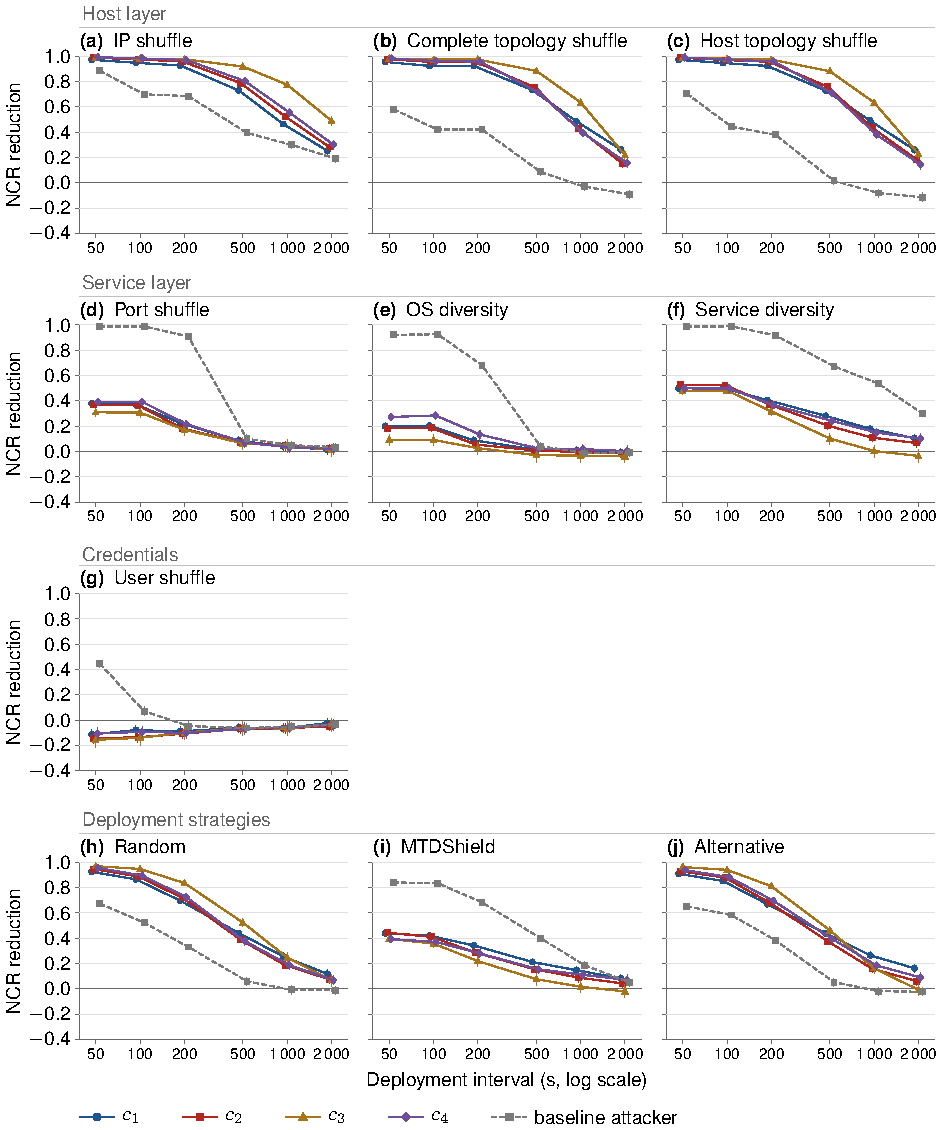
\includegraphics[height=0.80\textheight]{fig_5-3-3b_interval_mechanisms}\\
{\scriptsize At 50 to 200\,s the four attack profiles differ from one another less than the baseline attacker differs from the nearest of them (dissertation Figure 5.4).}
\end{frame}

% Table 6.1, Section 3.3.2, T7.
\begin{frame}{Backup: scoring the eight properties}
\centering
\small
\begin{tabular}{@{}l c c c c c c c c@{}}
\toprule
 & 1 & 2 & 3 & 4 & 5 & 6 & 7 & 8 \\
Attacker model & Pers. & Obj. & Strat. & Adapt. & Detect. & Cost & Learn. & Deploy. \\
\midrule
Baseline attacker (2023) & \yes & \no & part & part & \no & \no & \no & \no \\
Masud et al.\ (2025) & part & \no & \no & \no & \no & \no & \no & \no \\
Kim et al.\ (2026) & part & \no & \no & \no & part & \no & \no & \no \\
\textbf{APT attacker model} & \yes & part & \yes & part & part & \no & \no & \no \\
\bottomrule
\end{tabular}\\[2mm]
\raggedright
\begin{itemize}
  \item Each property split into predicates; \yes{} = every predicate true of the model's own behaviour; part = a behaviour predicate true, but set by a fixed rule or assumed
  \item One scorer, checked by blind scoring with language models (dissertation Appendix B)
  \item Adaptivity is in part because the failure matrix is a fixed rule of mine; detection avoidance in part because MTDSim has no IDS
\end{itemize}
\end{frame}

% Section 4.3, Equations 4.2 and 4.4, Figure 4.4.
\begin{frame}{Backup: the Petri net}
\begin{columns}[T]
\begin{column}{0.52\textwidth}
\centering
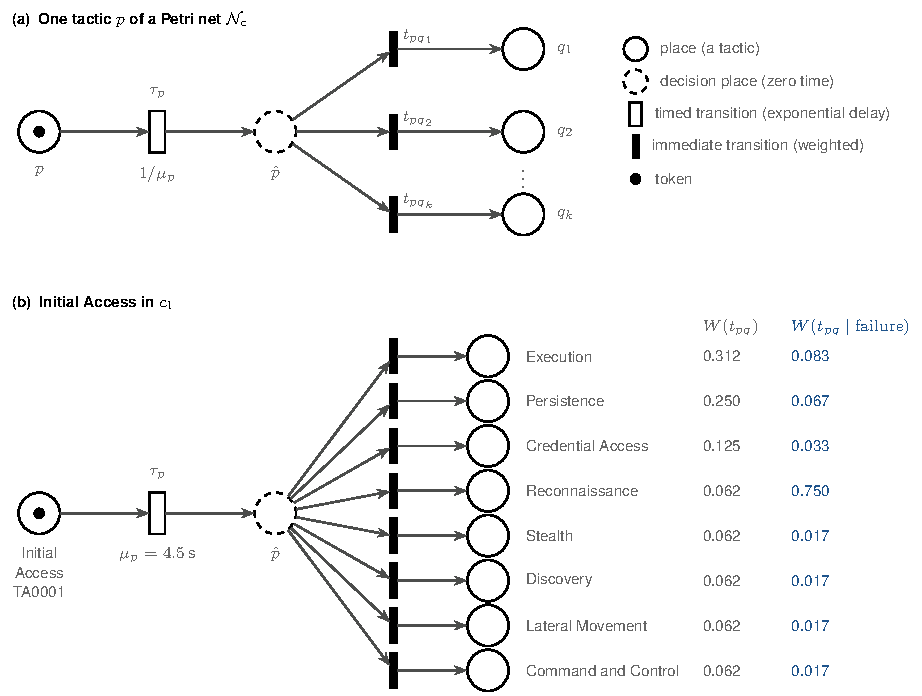
\includegraphics[width=\linewidth]{fig_4-3a_gspn_gadget}
\end{column}
\begin{column}{0.45\textwidth}
\small
Generalised stochastic Petri net \src{Ajmone Marsan 1995}, extended with the failure matrix $F$:
\[(P, T, I, O, W, M_0, F)\]
Base weight of the move from tactic $p$ to $q$:
\[W(t_{pq}) = \frac{n(p,q)}{\sum_{q'} n(p,q')}\]
with $n(p,q)$ the attack flows that draw $p \to q$. After a failed attack action:
\[W(t_{pq}\mid\text{failure}) = \frac{W(t_{pq})\,F(p,q)}{\sum_{q'} W(t_{pq'})\,F(p,q')}\]
One token, starting on Reconnaissance.
\end{column}
\end{columns}
\end{frame}

% Table 4.2, Figure 4.6.
\begin{frame}{Backup: tactic durations and the tactic-to-action mapping}
\begin{columns}[T]
\begin{column}{0.50\textwidth}
\small
\begin{tabular}{@{}>{\raggedright\arraybackslash}p{0.72\linewidth} r@{}}
\toprule
Tactics & Mean (s) \\
\midrule
Initial Access, Privilege Escalation, Credential Access, Lateral Movement {\scriptsize(MTDSim's exploit)} & 4.5 \\
Reconnaissance, Discovery {\scriptsize(MTDSim's three scans)} & 35 \\
Persistence, Stealth, Command and Control & 45 \\
Collection, Exfiltration, Impact & 36 \\
Execution, Defense Impairment & 22.5 \\
Resource Development & 0 \\
\bottomrule
\end{tabular}\\[1mm]
{\scriptsize Last four rows: judgement, kept on the baseline attacker's time scale and under the 200\,s default interval.}
\end{column}
\begin{column}{0.46\textwidth}
\centering
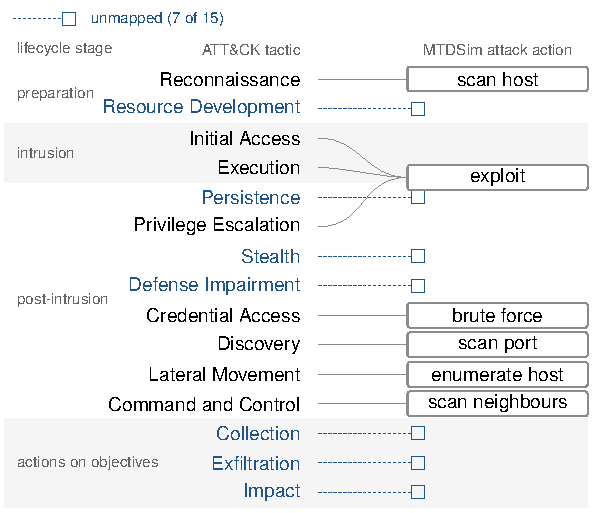
\includegraphics[width=\linewidth]{fig_4-4a_controller_mapping}
\end{column}
\end{columns}
\end{frame}

% Appendix E.4 and E.5.
\begin{frame}{Backup: MTDShield as run}
\begin{itemize}
  \item Run as released by Tay (2024); correcting the release would make it my agent, not Tay's
  \item Trained at one deployment interval, against the baseline attacker, on 100-host networks
  \item Known limits of the release: published scores produced with exploration at one; four evaluation inputs read as zero; ``do nothing'' never a learning target
  \item Its detection input reads an unmapped tactic as ``nothing detected''
  \item So the result bounds MTDShield \emph{as released}, not MTDShield retrained against the APT attacker model
\end{itemize}
\vfill{\scriptsize Dissertation Appendix E, threat T12.}
\end{frame}

% Figure 5.2; Appendix F.1, Table F.3.
\begin{frame}{Backup: disruption per MTD deployment, and ASP}
\begin{columns}[T]
\begin{column}{0.58\textwidth}
\centering
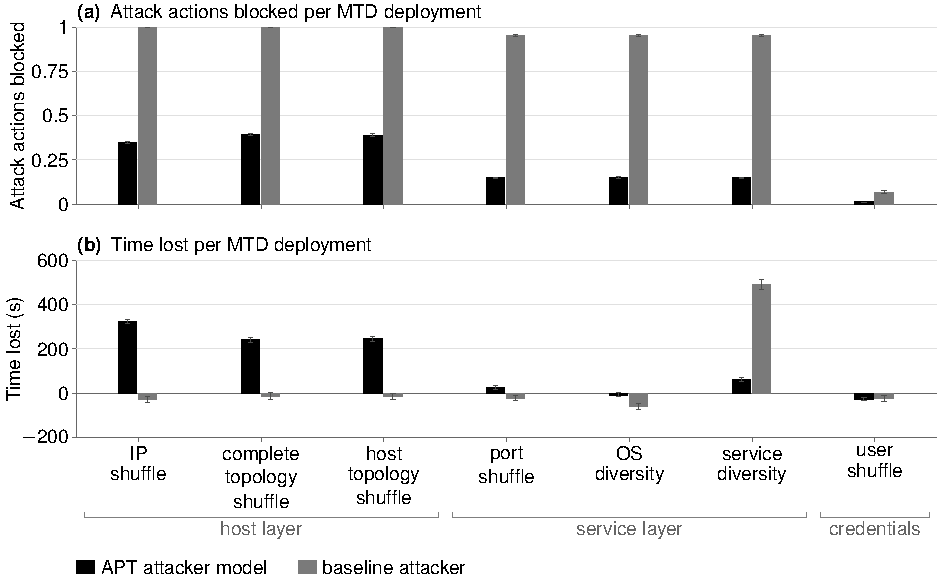
\includegraphics[width=\linewidth]{fig_5-2-2a_disruption_response}
\end{column}
\begin{column}{0.39\textwidth}
\begin{itemize}
  \item Measured at 2\,000\,s, because the next deployment caps time lost at the interval
  \item The baseline attacker's time lost is at or below zero after the first deployment: sent back to scan host, it gets a second attempt at its first host, as MTDSim intends
  \item On ASP reduction the layer order also holds against each attacker (Table F.3)
\end{itemize}
\end{column}
\end{columns}
\end{frame}

% T3.
\begin{frame}{Backup: verification, and why no comparison with earlier MTDSim numbers}
\begin{itemize}
  \item An event tracer replays any run step by step, across Petri net, attacker and MTD
  \item MTDSim's code audited against what its papers describe; unit tests of the Petri net and the simulator
  \item Fixed seeds reproduce every run exactly
  \item Defects found in MTDSim were repaired before the evaluation, so results are not compared numerically with Zhang (2023) or Tay (2024)
\end{itemize}
\vfill{\scriptsize Dissertation threat T3.}
\end{frame}

\begin{frame}{References}
\scriptsize
\begin{itemize}
  \item[] A.~Alshamrani et al., ``A survey on advanced persistent threats,'' \emph{IEEE Commun.\ Surveys Tuts.}, 21(2), 2019.
  \item[] M.~Ajmone Marsan et al., \emph{Modelling with Generalized Stochastic Petri Nets}, Wiley, 1995.
  \item[] A.~Brown, T.-W.~Lee and J.~B.~Hong, ``Evaluating moving target defenses against realistic attack scenarios,'' EnCyCriS, 2023.
  \item[] Center for Threat-Informed Defense, ``Attack Flow,'' MITRE, v3.2.0, 2025.
  \item[] J.-H.~Cho et al., ``Toward proactive, adaptive defense: A survey on moving target defense,'' \emph{IEEE Commun.\ Surveys Tuts.}, 22(1), 2020.
  \item[] CISA et al., ``PRC state-sponsored actors compromise and maintain persistent access to U.S.\ critical infrastructure,'' Advisory AA24-038A, 2024.
  \item[] {\L}.~Jalowski et al., ``Rethinking the security assurances of MTD: A gap analysis for network defense,'' \emph{Future Internet}, 18(2), 2026.
  \item[] M.~Kim et al., ``MTD in depth: Multi-phased moving target defense techniques against cyber-attacks based on cyber kill chain,'' \emph{FGCS}, 181, 2026.
  \item[] M.~T.~Masud et al., ``Vulnerability defence using hybrid moving target defence in Internet of Things systems,'' \emph{Computers \& Security}, 153, 2025.
  \item[] Joint Task Force, ``Managing information security risk,'' NIST SP 800-39, 2011.
  \item[] C.~Tantithamthavorn et al., ``An empirical comparison of model validation techniques for defect prediction models,'' \emph{IEEE TSE}, 43(1), 2017.
  \item[] J.~K.~Tay, ``Using artificial intelligence to automate the deployment of moving target defence operations,'' UWA research report, 2024.
  \item[] W.~Zhang, ``Evaluating multiple moving target defence in the time domain,'' Master's thesis, UWA, 2023.
\end{itemize}
\end{frame}

\end{document}
